\documentclass{book}

\usepackage{graphicx}
\usepackage{moreverb}
\usepackage{amsmath}
\usepackage{alltt}
\usepackage{rotating}
\usepackage{subfigure}
\usepackage{toc}
\usepackage{xspace}
\usepackage{makeidx}

\usepackage[T1]{fontenc}   % so _, <, and > print correctly in text.
\usepackage[dvips,colorlinks=true]{hyperref}  % This must be the last package

\newcommand{\sref}[1]{\S\ref{#1}}
\newcommand{\Sref}[1]{Sec.~\sref{#1}}

\newcommand{\vn}{\begingroup\catcode`\_=11 \catcode`\%=11 \dottcmd}
\newcommand\dottcmd[1]{{\usefont{T1}{lmss}{bx}{n} #1}\endgroup}

\newenvironment{example}
  {\vspace{-3.0ex} \begin{alltt}}
  {\end{alltt} \vspace{-2.5ex}}


\definecolor{light-gray}{gray}{0.95}
\lstset{backgroundcolor=\color{light-gray}}
\lstset{xleftmargin=0cm}
\lstset{framexleftmargin=0.3em}

\lstnewenvironment{Xcode}{}{}

\definecolor{lightcyan}{rgb}{0.88, 1.0, 1.0}
\newcounter{main}
\setcounter{main}{1}
\lstnewenvironment{code}[1][firstnumber=\themain,name=main]
  {\lstset{ %language=haskell,
           %columns=fullflexible,
           columns=fixed,
           basicstyle=\small\ttfamily,
           %numbers=left,
           numberstyle=\tiny\color{gray},
           backgroundcolor=\color{lightcyan},
           #1
          }
}
{\setcounter{main}{\value{lstnumber}}}



\setlength{\textwidth}{6.25in}
\setlength{\oddsidemargin}{0.25in}
\setlength{\evensidemargin}{0.00in}
\setlength{\textheight}{8.5in}
\setlength{\topmargin}{0in}

\makeindex

\begin{document}

\index{Lattice!model|see{Model Lattice}}
\index{Lattice!design|see{Design Lattice}}
\index{Lattice!base|see{Base Lattice}}

\thispagestyle{empty}

\begin{flushright}
\large
  Revision: 9.8.1 \\
  January 18, 2008 \\
\end{flushright}

\vfill

{
\begin{center}
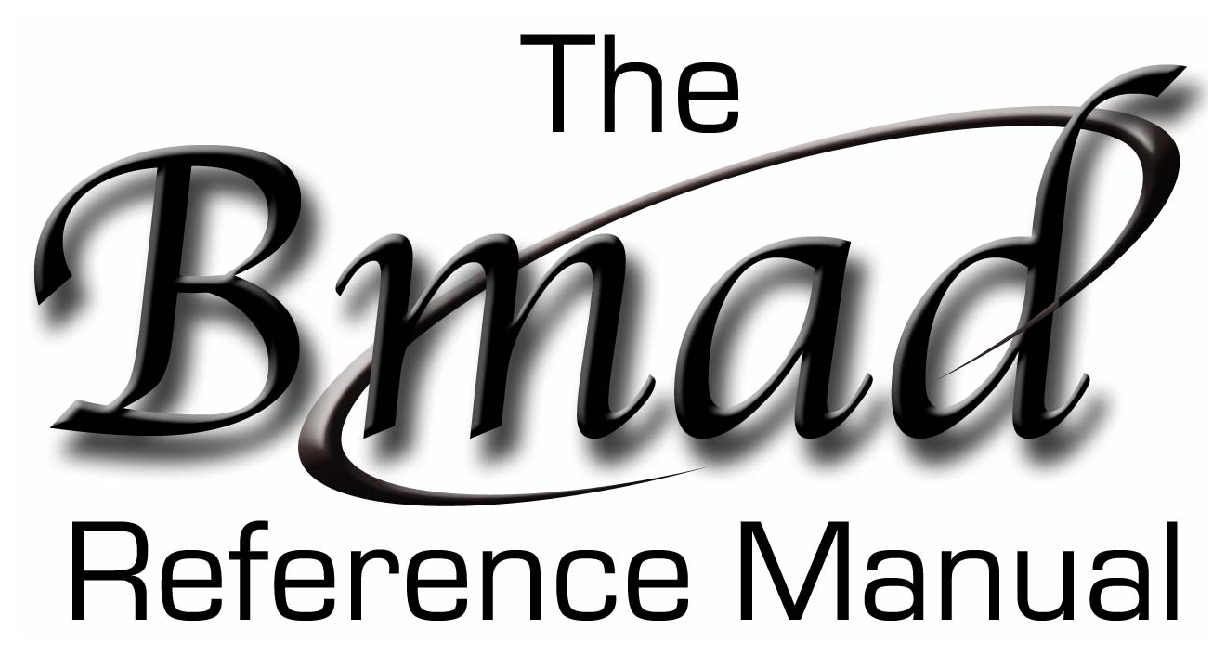
\includegraphics[width=12cm]{bmad-ref-manual.eps} \\
\vskip 0.3in
\huge\bf David Sagan
\end{center}
}

\vfill
\break



%----------------------------------------------------------------
{
\setlength{\parskip}{\dPar}
\setlength{\parindent}{0ex}

\chapter{Introduction}
\label{c:introduction}

%----------------------------------------------------------------
\section{Obtaining Tao}
\index{tao!Obtaining}
\label{s:obtaining}

A \vn{Distribution} is a set of files, including \bmad and \tao source files, which are used to
build the \bmad, the \tao program, and various other simulation programs. A \vn{Release} is like a
\vn{Distribution} except that it is created on the Linux computer system at CLASSE (Cornell's
Laboratory for Accelerator-based Sciences and Education). More information can be obtained from the
\bmad web site. 

If there is no local \bmad Guru to guide you, download and setup instructions for downloading a
Distribution, environment variable setup, and building \tao is contained on the \bmad web
site and will not be covered here.

%----------------------------------------------------------------
\section{Starting and Initializing Tao}
\index{initializing!files}
\label{s:initializing}

The syntax for starting \tao is given in \Sref{s:command.line}.

Initialization occurs when \tao is started. Initialization information is stored in one or more
files as discussed in Chapter \sref{c:init}.

%%----------------------------------------------------------------
\section{Running Tao with OpenMP}
\index{openMP}
\label{s:openmp}

\vn{OpenMP} is a standard that enables programs to run calculations with multiple threads which will
reduce computation time. Certain calculations done by \tao, including beam tracking and dynamic
aperture calculations, can be run multithreaded via OpenMP if the \tao executable file has been
properly compiled.  Interested users should consult their local \bmad Guru for guidance. Note:
\vn{OpenMP} multithreading involves using multiple cores of a single machine (unlike \vn{Open MPI}
which involves multiple machines). Therefore, it is not necessary to have a cluster of machines to
use \vn{OpenMP}.

To set the number of threads when running a program compiled with \vn{OpenMP}, set the environment variable
\vn{OMP_NUM_THREADS}. Example:
\begin{example}
  export OMP_NUM_THREADS=8
\end{example}

This may also be set during Tao runtime as the global parameter \vn{n_threads}. For example:
\begin{example}
  set global n_threads = 1  ! Use only a single thread
  set global n_threads = 4  ! Use four threads
\end{example}

See \sref{s:set.global} for more information.

To the local \bmad Guru: Compiling and linking of \tao with \vn{OpenMP} is documented on the \bmad
web site. By default, \vn{OpenMP} is not enabled. Essentially, OpenMP is enabled by modifying
the \vn{dist_prefs} file before compiling and linking.

%----------------------------------------------------------------
\section{Command Line Mode and Single Mode}
\label{s:modes}

After \tao is initialized, \tao interacts with the user though the command line. \tao has two modes
for this. In \vn{command line} mode, which is the default mode, \tao waits until the the \vn{return}
key is depressed to execute a command. Command line mode is described in Chapter~\sref{c:command}. 

In \vn{single} mode, single keystrokes are interpreted as commands. \tao can be set up so that in
\vn{single mode} the pressing of certain keys increase or decrease variables. While the same effect
can be achieved in the standard \vn{line mode}, \vn{single mode} allows for quick adjustments of
variables. See Chapter~\sref{c:single} for more details.

%-----------------------------------------------------------------
\section{Lattice Calculations}
\index{lattice calculaitons}
\label{s:lat.calc.overview} 

By default \tao recalculates lattice parameters and does tracking of particles after each command.
The exception is for commands that do not change any parameter that would affect such calculations
such as the \vn{show} command. See \sref{s:lat.calc} for more details. If the recalculation takes a
significant amount of time, the recalculation may be suppressed using the \vn{set global
lattice_calc_on} command (\sref{s:set.global}) or the \vn{set universe} command
(\sref{s:set.universe}).

%-----------------------------------------------------------------
\section{Command Files and Aliases}
\index{command files}
\label{s:command.files} 

Typing repetitive commands in command line mode can become tedious. \tao has two constructs to
mitigate this: Aliases and Command Files. 

Aliases are just like aliases in Unix. See Section~\sref{s:alias} for more details.

Command files are like Unix shell scripts. A series of commands are
put in a file and then that file can be called using the \vn{call}
command (\sref{s:call}).

\tao will call a command file at startup. The default name of this startup file is \vn{tao.startup}
but this name can be changed (\sref{s:format}).

Do loops (\sref{s:do}) are allowed with the following syntax:
\begin{example}
  do <var> = <begin>, <end> \{, <step>\} 
    ...
    tao command [[<var>]]
    ...
  enddo
\end{example}
The \vn{<var>} can be used as a variable in the loop body but must be
bracketed ``[[<var>]]''.  The step size can be any integer positive or
negative but not zero.  Nested loops are allowed and command files can
be called within do loops.

\begin{example}
  do i = 1, 100
    call set_quad_misalignment [[i]] ! command file to misalign quadrupoles
    zero_quad 1e-5*2^([[i]]-1) ! Some user supplied command to zero quad number [[i]]
  enddo
\end{example}

To reduce unnecessary calculations, the logicals \vn{global%lattice_calc_on}
and \vn{global%plot_on} can be toggled from within the command file. Also 
setting \vn{global%quiet} can turn off verbose output to the terminal. Example
\begin{example}
  set global quiet = all          ! Turn off verbose output to the terminal.
  set global lattice_calc_on = F  ! Turn off lattice calculations
  set global plot_on = F          ! Turn off plot calculations
  ... do some stuff ...
  set global plot_on = T          ! Turn back on 
  set global lattice_calc_on = T  ! Turn back on
  set global quiet = off         
\end{example}
See \sref{s:globals} for more details.

A \vn{end_file} command (\sref{s:end.file}) can be used to signal the
end of the command file.

The \vn{pause} command (\sref{s:pause}) can be used to temporarily
pause the command file.


}

%----------------------------------------------------------------
\tableofcontents
\listoffigures
\listoftables

%----------------------------------------------------------------
\setlength{\parskip}{\dPar}
\setlength{\parindent}{0ex}

\part{Concepts and Tutorial}

\chapter{Tao Concepts}
\label{c:concepts}

\tao stands for ``Tool for Accelerator Optics''. \tao is a general
purpose program for simulating high energy particle beams in
accelerators and storage rings. This tutorial assumes you are already
familiar with the basics of particle beam dynamics and its
formalism. There are several books that introduce the topics very
well. A good place to start is \textit{The Physics of Particle
Accelerators} by Klaus Wille.

\index{Bmad}
\tao is based on the \bmad\cite{b:bmad} subroutine library. An
understanding of the nitty-gritty details of the routines that
comprise \bmad is not necessary, however, one should be familiar with
the conventions that \bmad uses and this is covered in the \bmad
manual.

So, what is \tao good for? A large variety of applications. It's
versatility is that it's easily expandable. Think of it as an
accelerator design and analysis environment. But even without any
customizations, \tao will do much analysis. 

This chapter discusses how \tao is organized. After you are familiar
with the basics of \tao, there is a hands-on tutorial in
Chapter~\sref{c:tutorial}. After you get more familiar with \tao, you
might be interested exploit its versatility by extending \tao to do
custom calculations. For this, see Chapter~\ref{c:custom.tao}.

%----------------------------------------------------------------
\section{The Organization of Tao: The Super\_Universe}
\label{s:organization}

Many simulation problems fall into one of three categories: 
\begin{itemize}
\item 
Design a lattice subject to various constraints.
\item
Simulate errors and changes in machine parameters. For example, you want to
simulate what happens to the orbit, beta function, etc., when you change
something in the machine. 
\item 
Simulate machine commissioning including simulating data measurement and
correction. For example, you want to know what steering strength changes will
make an orbit flat.
\end{itemize}
Programs that are written to solve these types of problems have common
elements: You have variables you want to vary in your model of your
machine, you have "data" that you want to view, and, in the first two
categories above, you want to match the machine model to the data (in
designing a lattice the constraints correspond to the data).

With this in mind, \tao was structured to implement the essential
ingredients needed to solve these simulation problems.  
The information that \tao knows about can be divided into five
(overlapping) categories:
\begin{description}
  \index{Lattice}
  \item[Lattice] \Newline   
Machine layout and component strengths, and the beam orbit (\sref{s:lattice}).
  \index{Data}
  \item[Data] \Newline
Anything that can be measured.
For example: The orbit of a particle or the lattice beta 
functions, etc. (\sref{c:data})
  \index{Varialbe}
  \item[Variables] \Newline
Essentially, any lattice parameter or initial condition that can be varied.
For example: quadrupole strengths, etc. (\sref{s:variable.overview}).
  \index{Plotting}
  \item[Plotting]  \Newline
Information used to draw graphs, display the lattice 
floor plan, etc. (\sref{s:plotting}).
  \index{Global parameters}
  \item[Global Parameters] \Newline
 \tao has a set of parameters to control every aspect of how it behavies from
the random number seed \tao uses to what optimizer is used for fitting data.
\end{description}

%------------------------------------------------------------------------
\section{The Super\_universe}
\label{s:super.uni}
\index{Super_universe}
\index{Structure}
The information in \tao deals is organized in a hierarchy of
\vn{``structures''}. At the top level, everything known to \tao is
placed in a single structure called the \vn{super_universe}.

Within the \vn{super_universe}, lies one or more \vn{universes}
(\sref{s:universe}), each \vn{universe} containing a particular
machine lattice and its associated data. This allows for the user to
do analysis on multiple machines or multiple configurations of a
single machine at the same time. The \vn{super_universe} also contains
the \vn{variable}, \vn{plotting}, and \vn{global parameter} information.

%------------------------------------------------------------------------
\section{The Universe}
\label{s:universe}
\index{Universe!textbf}

\index{Lattice}\index{Design lattice}\index{Model lattice}\index{Base lattice}
\index{Data}
The \tao \vn{super_universe} (\sref{s:super.uni}) contains one or
more \vn{universes}.  A \vn{universe} contains a \vn{lattice}
(\sref{s:lattice}) plus whatever data (\sref{c:data}) one wishes to
study within this lattice (i.e. twiss parameters, orbit, phase,
etc.). Actually, there are three lattices within each universe: the
\textbf{design} lattice, \textbf{model} lattice and \textbf{base}
lattice. Initially, when \tao is started, all three lattices are
identical and correspond to the lattice read in from the lattice
description file (\sref{s:init.lat}).

There are several situations in which multiple universes are
useful. One case is where there are multiple machines. For example, a
transfer line connected to a storage ring. In this case, one universe
will correspond to the transfer line and another universe will
correspond to the storage ring. 

Another case where multiple universes are useful is where data has
been taken under different machine conditions. For example, suppose
that a set of beam orbits have been measured in a storage ring with
each orbit corresponding to a different steering element being set to some
non-zero value. To determine what
quadrupole settings will best reproduce the data, multiple universes can be
setup, one universe for each of the orbit measurements. Variables can be
defined to simultaneously vary the corresponding quadrupoles in each
universe and \tao's built in optimizer can vary the variables until
the data as determined from the \vn{model} lattice (\sref{s:lattice})
matches the measured data. This \vn{orbit response matrix} (ORM) analysis
is, in fact, a widly used procedure at many laboratories.

%------------------------------------------------------------------------
\section{Lattices}
\index{Lattice!textbf}
\label{s:lattice}

A \vn{lattice} consists of a machine description (the strength and
placement of elements such as quadrupoles and bends, etc.), along with the
beam orbit through them. There are actually three types of lattices:
  \vspace*{-3ex}
  \begin{description}
  \index{Design lattice!textbf}
  \item[Design Lattice] \Newline 
The \vn{design} lattice corresponds to the lattice read in from the
lattice description file(s) (\sref{s:init.lat}). In many instances, this
is the particular lattice that one wants the actual physical machine
to conform to. The \vn{design} lattice is fixed. Nothing is allowed to
vary in this lattice.
  \index{Model lattice!textbf}
  \item[Model Lattice] \Newline
Except for some commands that explicitly set the \vn{base} lattice,
all \tao commands to vary lattice variables vary quantities in the
\vn{model} lattice. In particular, things like orbit correction
involve varying \vn{model} lattice variables until the \vn{data},
as calculated from the \vn{model}, matches the \vn{data} as actually measured.
  \index{Base lattice!textbf}
  \index{Base lattice!using set command}
  \item[Base Lattice] \Newline
It is sometimes convenient to designate a reference lattice so that
changes in the \vn{model} from the reference point can be examined.
This reference lattice is called the \vn{base} lattice. The \vn{set}
command (\sref{s:set}) is used to transfer information from the
\vn{design} or \vn{model} lattices to the base lattice.
  \end{description}

%------------------------------------------------------------------------
\section{Variables}
\label{s:variable.overview}
\index{Variables}

\index{Change command}
\index{Optimizer!variables}
A variable is anything that can be varied. For example, quadrupole
strengths or the initial position of a particle in a LINAC. Any
variable can be varied using the \vn{change} command
(\sref{s:change}). However it can be convenient to set up within \tao
predefined groups of variables. For example, the optimizer
(\sref{s:optimizer}) will only work with such blocks.

Variables control attributes of elements in the model lattice of one
or more universes. They are not the same thing as attributes in
lattice elements.  Instead, they \textit{control} attributes in
lattice elements. They are more akin to \bmad \textit{overlays}. A
given variable may control a single attribute of one element in one or
more universes. If you want a variable to control a collection of
elements like a \bmad \textit{group} then you need to insert the
appropriate group element in your lattice. Variables are what you vary in
order to change your model lattice. You can also change your model
lattice by directly changing and lattice element attribute. However,
if you plan on doing any optimization then you will need to use
variables.

\index{Variables!v1_var}
Blocks of variables are associated with what is called a \vn{v1_var}
structure and each of these structures has a \vn{name} with which to
refer to them in \tao commands. For example, if \vn{quad_k1} is the
name of a \vn{v1_var}, then \vn{quad_k1[5]} referres to the variable 
with index 5 in the block. 

A set of variables within a \vn{v1_var} block
can be referred to by using using a comma \vn{,} to
separate their indexes. Additionally, a colan \vn{:} can be use to
specify a range of variables. For example
\begin{example}
  quad_k1[3:6,23]
\end{example}
refers to variables 3, 4, 5, 6, and 23. Instead of a number, the
associated lattice element name can be used so if, in the above
example, the lattice element named \vn{q01} is assocaited with
\vn{quad_k1[1]}, etc., then the following is equivalent:
\begin{example}
  quad_k1[q03:q06,q23]
\end{example}
Using lattice names instead of numbers is not valid if the same
lattice element is associated with more than one variable in a
\vn{v1_var} array. This can happen, for example, if one variable controls
an element's \vn{x_offset} and another variable controlls the same element's
\vn{y_offset}. 

In referring to variables, a ``\vn{*}'' can be used as a wild card to 
denote ``all''. Thus:
\begin{example}
  *                ! All the variables
  quad_k1[*]|model ! All model values of quad_k1.
  quad_k1[]|model  ! No values. That is, the empty set.
  quad_k1|model    ! Same as quad_k1[*]|model
\end{example}

A given variable may control a single attribute of one element in a
\vn{model} lattice of a single universe or it can be configured to
simultaneously control an element attribute across multiple
universes. Any one variable cannot control more than one attribute of
one element. However, a variable may control an overlay or group
element which, in turn, can control numerous elements.

Each individual variable has a number of values associated with it:
  \vspace*{-3ex}
  \index{Variable!measured}\index{Variable!reference}
  \index{Variable!model}\index{Variable!design}\index{Variable!base}
  \begin{description}
  \item[Measured Value] \Newline
The Value as obtained at the time of the \vn{data} measurement.
  \item[Reference Value] \Newline
The Value as obtained at the time of the \vn{reference} data  measurement.
  \item[Model Value] \Newline
The value as given in the \vn{model} lattice.
  \item[Design Value] \Newline
The value as given in the \vn{design} lattice.
  \item[Base Value] \Newline
The value as given in the \vn{base} lattice.
  \end{description}
These components and others can be refered to using the notaion
\vn{|name} where \vn{name} is the appropriate name for the
component. The list of components that can be set or refered to are:
\begin{example}
  quad_k1[1]|meas      ! Value at time of data measurement
  quad_k1[1]|ref       ! VAlue at time of the reference data measurement
  quad_k1[1]|model     ! Value in the model lattice
  quad_k1[1]|base      ! Value in the base lattice
  quad_k1[1]|design    ! Value in  the design lattice
  quad_k1[1]|weight    ! Weight used in the merit function.
  quad_k1[1]|old       ! Scratch value.
  quad_k1[1]|step      ! For fitting/optimization: What is considered a small change.
  quad_k1[1]|exists    ! Logical
  quad_k1[1]|good_var  ! Logical
  quad_k1[1]|good_ref  ! Logical
  quad_k1[1]|good_user ! Logical
  quad_k1[1]|good_opt  ! Logical
  quad_k1[1]|good_plot ! Logical
\end{example}

Use the \vn{show var} (\sref{s:show}) command to view variable information

%------------------------------------------------------------------------
\section{Plotting}\index{Arithmetic Expressions}
\label{s:arithmetic}

\tao is able to handle arithmetic expressions within commands
(\sref{c:command}) and in strings in a \tao initialization file.
Arithmetic expressions can be used in a place where a real value or an
array of real values are required.  The standard operators are
defined: \hfil\break \hspace*{0.15in}
\begin{tabular}{ll}
  $a + b$           & Addition        \\
  $a - b$           & Subtraction     \\
  $a \, \ast \, b$  & Multiplication  \\
  $a \; / \; b$     & Division        \\
  $a \, \land \, b$ & Exponentiation  \\
\end{tabular} \newline
The following intrinsic functions are also recognized: \hfil\break
\index{Intrinsic functions}
\hspace*{0.15in}
\begin{tabular}{ll}
  \vn{sqrt}(x)      & Square Root    \\
  \vn{log}(x)       & Logarithm      \\
  \vn{exp}(x)       & Exponential    \\
  \vn{sin}(x)       & Sine           \\
  \vn{cos}(x)       & Cosine         \\
  \vn{tan}(x)       & Tangent        \\
  \vn{asin}(x)      & Arc sine       \\
  \vn{acos}(x)      & Arc cosine     \\
  \vn{atan}(x)      & Arc Tangent    \\
  \vn{abs}(x)       & Absolute Value \\
  \vn{ran}()        & Random number between 0 and 1 \\
  \vn{ran_gauss}()  & Gaussian distributed random number with unit RMS \\
\end{tabular} \newline
Both \vn{ran} and \vn{ran_gauss} use a seeded random number generator. 
Setting the seed is described in Section~\sref{s:globals}.

When combining components from the same datum or variable in an
expression, the common prefix can be eliminated. For example
\begin{example}
  orbit.x[2:7,8]|model - 2*orbit.x[2:7,8]|meas
\end{example}
is equivalent to
\begin{example}
  orbit.x[2:7,8]|model - 2*meas
\end{example}

%------------------------------------------------------------------------
\section{Plotting}\index{Plotting}
\label{s:plotting}

\begin{figure}[tb]
  \centering
  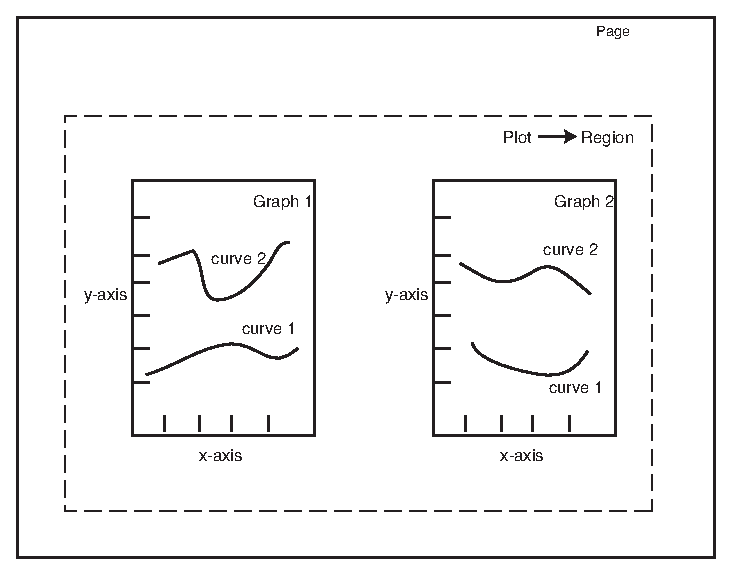
\includegraphics{plot.eps}
  \caption[A plot has a collection of graphs.]
{A plot has a collection of graphs and a graph has a 
collection of curves. A plot becomes visible when it is associated
with some region on the page using the \vn{place} command. Note that
on the actual page the plot/region border is not visible.}
  \label{f:plot}
\end{figure}

Some definitions:
  \vspace*{-3ex}
\begin{description}
\index{Curve|textbf}
\item[Curve] \Newline
A \vn{curve} is a set of (x,y) points to be plotted.
\index{Graph|textbf}
\item[Graph] \Newline
A \vn{graph} consists of horizontal and vertical axes along with a set
of \vn{curve}s that are plotted within the graph. 
\index{Plot|textbf}
\item[Plot] \Newline
A \vn{plot} is essentially a collection of \vn{graphs}.
\index{Page|textbf}
\item[Page] \Newline
The \vn{page} refers to the Xwindow where graphics are displayed or the 
corresponding printed graphics page.
\index{Region}
\item[Region] \Newline
The \vn{page} is divided up into a number of rectangles called
\vn{regions}. \vn{Regions} may overlap.
\end{description}

\index{Template plot}\index{Region}\index{Place command}
\index{Graph}\index{Plot!initialization file}\index{Curve}
The plot initialization file (cf.~Chapter~\ref{c:init}) defines a set
of \vn{template plots}. A \vn{template} defines what type of data is
to be plotted (orbit, beta function, etc.), how many \vn{graphs} there are,
what the scales are for the \vn{graph} axes, how the \vn{graph}s are
laid out, etc.  The plot initialization file also defines a set of
\vn{region}s within the \vn{page}. Any \vn{template plot} can be
placed in any region. Using the \vn{place} command (see
Chapter~\ref{c:command} for a full descriptions of all commands) one
can assign a particular \vn{template plot} to a particular region for
plotting.  The relationship between \vn{region}, \vn{plot},
\vn{graph}, and \vn{curve} is shown graphically in
Figure~\ref{f:plot}.

Figures~\ref{f:plot.page1} and \ref{f:plot.page2} show examples of a
plot \vn{page}. Figure~\ref{f:plot.page1} was generated by defining
two regions called \vn{top} and \vn{bottom} in the plot initialization
file. The \vn{top} region was defined to cover the upper half of the
\vn{page} and the \vn{bottom} region was defined to cover the bottom
half. \vn{Template plots} were defined to plot phase and orbit data
from a defined set of detector elements in the lattice. Each
\vn{template plot} defined two graphs which in both cases where
assigned the names \vn{x} and \vn{y}. The orbit \vn{template plot} was
placed in the \vn{top} region and the phase \vn{template plot} was
placed in the \vn{bottom} region. The horizontal axis numbering is by
detector \vn{index}.  Displayed plots are referred to by the
\vn{region} name (\vn{top} and \vn{bottom} in this case). Individual
graphs and curves are referred to using the nomenclature
\vn{region.graph.curve}. Thus, in this example, the horizontal orbit graph
would be referred to as \vn{top.x}.  Using the \vn{plot} command one
can then specify \vn{who} is plotted. \vn{who} refers to
\vn{measured}, \vn{reference}, \vn{model}, \vn{base}, and/or
\vn{design} data.  Notice that the same \vn{template plot} can be
assigned to different \vn{regions} and the plots in different
\vn{regions} can have different scales for their axes or different
\vn{who}. In the example in Figure~\ref{f:plot.page1}, \vn{who} for
the \vn{top} plot is \vn{model} and for the \vn{bottom} plot it is
\vn{model - design}.

Plots may be referred to by their template name or by the name of the
region they are placed in. For example, the orbit plot in
Figure~\ref{f:plot.page1} may be referred to using the region name
(\vn{top}) or the template name (\vn{orbit}). A template may be placed
in multiple regions.  For example, you may wish to plot the \vn{model}
data for the orbit in one region and the \vn{design} data for the
orbit in another region. In this case the command \vn{scale orbit}
would scale the plots in both regions while to scale the plot in only
one of the regions you would need to use the region name. A graph of a
plot is specified using the format \vn{plot_name.graph_name} where
\vn{plot_name} is a template or region name and \vn{graph_name} is the
name of the graph. For example, if the horizontal orbit graph of the
]\vn{orbit} plot is named \vn{x} then it would be referred to as
\vn{orbit.x} or \vn{top.x}. A curve within a graph is specified using
the format \vn{plot_name.graph_name.curve_name}.

The \vn{use}, \vn{veto}, \vn{restore}, and \vn{clip} commands are used
to control what data is used in fitting the model to the data in the
optimization process (see Chapter~\ref{c:opti}). The general rule is
that these commands only effect measured and reference data. If
plotting \vn{model}, \vn{design} and/or \vn{base} data then the data
will be displayed irregardless. If plotting \vn{meas} and/or \vn{ref} data
then the data displayed will vary with these commands.  \vn{meas} or
\vn{ref} data vetoed for display is also vetoed for fitting.  However,
measured data that is off the vetical or horizontal scale may still be
used by the optimizer unless vetoed with the \vn{veto} or \vn{clip}
command.  If there are data points off the vertical scale then
``**Limited**'' will appear in the upper right-hand corner of the
graph. If plotting measured data then these points off scale will
still be used by the optimizer.

The \vn{x-axis} and \vn{x-scale} commands are used to set the axis
type and scale for each graph. The axis type can be either \vn{index},
\vn{ele_index} or \vn{s} which corresponds to the data index number,
element index number and longitudinal poisition in the lattice (from
element 0) respectively.

Figure~\ref{f:plot.page2} shows another example of a plot \vn{page}.
In this case the \vn{page} was generated by again defining two
vertically stacked regions but in this case the regions have different
heights.  A \vn{template plot} with a single graph was placed in the
bottommost \vn{region}.  This \vn{graph} contains a \vn{key_table}.
A \vn{key_table} is used in conjunction with \vn{single mode} and is
explained in Chapter~\ref{c:single}. A \vn{template plot} containing
five \vn{graphs} was placed in the uppermost region. The uppermost
\vn{graph} of this \vn{template plot} contains a \vn{lat_layout} which
shows the placement of lattice elements.  What elements are displayed
in a \vn{lat_layout} and what shapes they are represented by is
specified in the initialization file. The horizontal scale is
longitudinal position (\vn{s}).  The remaining four graphs show
dispersion and beta data from two different universes representing the
low energy and high energy transport in an energy recovery linac. The
individual data points here (hard to see in this example) have been
slaved to the \vn{lat_layout} and represent the beta and dispersion at
the edges of the displayed elements in the \vn{lat_layout}.


\begin{figure}
  \centering
  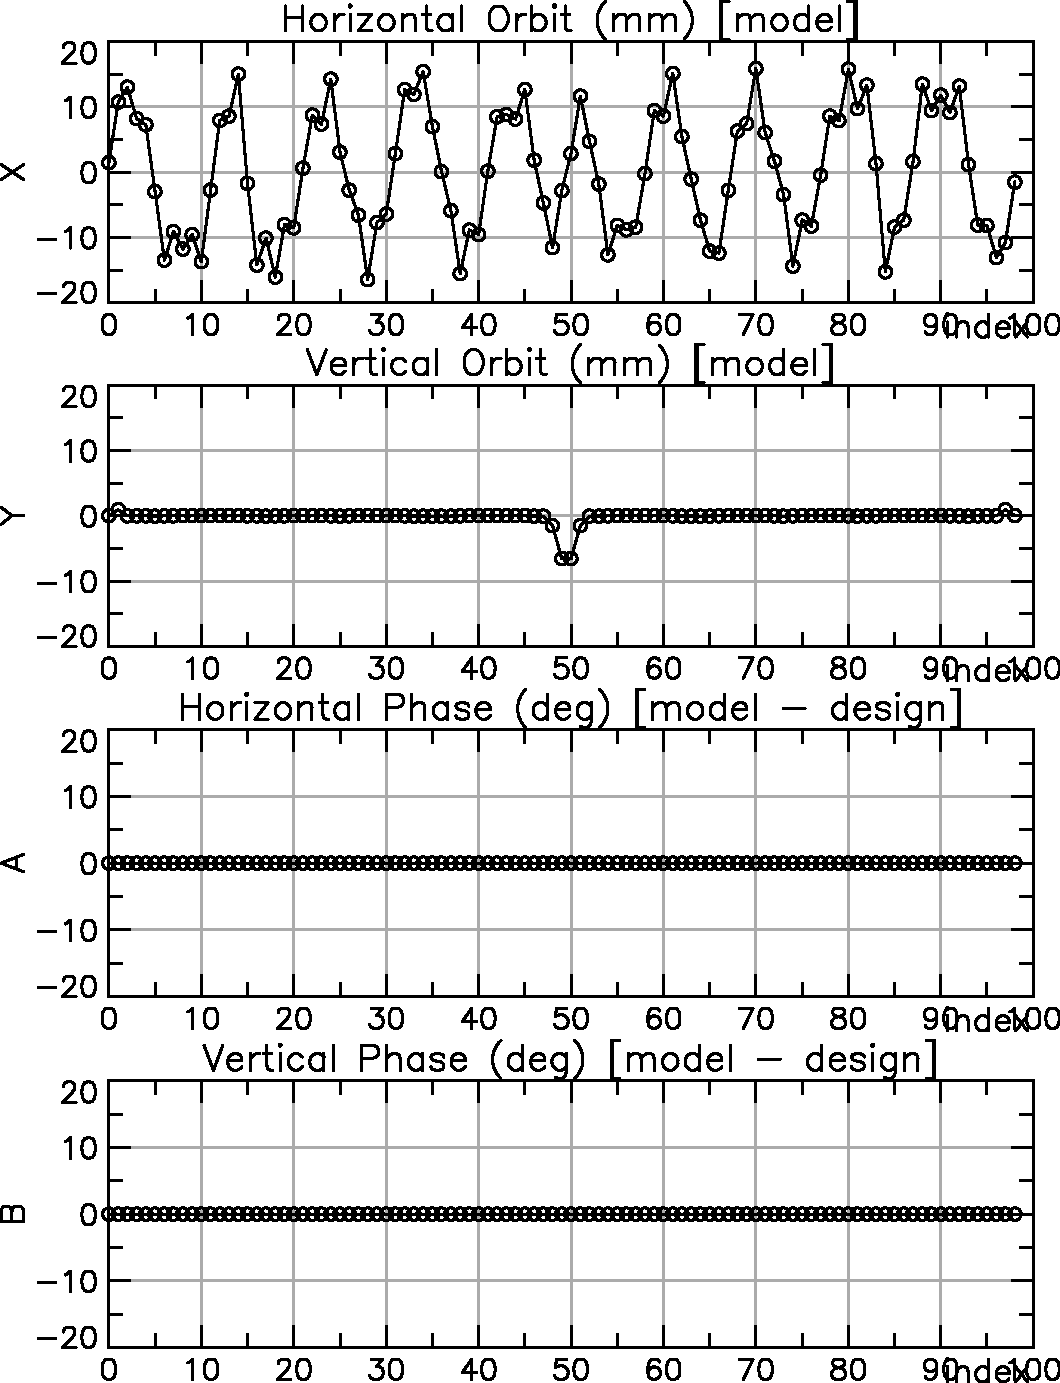
\includegraphics[width=5in]{plot-page1.eps}
  \caption{Example of a plot page}
  \label{f:plot.page1}
\end{figure}

\begin{figure}
  \centering
  \includegraphics[width=5in]{plot-page2.eps}
  \caption{Another example of a plot page.}
  \label{f:plot.page2}
\end{figure}

\vfill
\break
%------------------------------------------------------------------------
\section{Single Character Input}
\index{Single Mode}

Sometimes it is convenient to be able to vary variables using single
key strokes without having to type a carriage return.  With \tao, this
is possible using what is called \vn{single mode}. This is distinct
from \vn{line mode} where commands to \tao are typed at the command
line with a carriage return signaling the end of the command. 

The \vn{single mode} initialization file associates variables with
certain keyboard keys so that when these keys are pressed the value of
the variable is varied. This association between variables and keys is
called a \vn{key table}. See Chapter~\sref{c:single} for more details.

%------------------------------------------------------------------------
\section{Tracking Types}
\index{Tracking!Types}

\index{track_type}
\index{tao_global_struct}
\index{Global%track_type}
The are two types of tracking implemented in \tao: single particle
tracking and many particle multi-bunch tracking.
Single particle tracking is just that, the
tracking of a single particle through the lattice. Many particle
multi-bunch tracking creates a gaussian distribution of particles at
the beginning of the lattice and tracks each particle through the
lattice, including any wakefields. 
Single particle tracking is used by default. The
\vn{global%track_type} parameter (\sref{s:globals}), which is set in
the initialization file, is used to set the tracking.

Particle spin tracking has also been set up for single particle and many
particle tracking. See Sections~\sref{s:globals} and \sref{s:beam.init} for
details on setting up spin tracking.

%------------------------------------------------------------------------
\section{Lattice Calculation}\index{Lattice!calculation of}
\label{s:lat.calc}

After each \tao command is processed, the lattice and ``merit''
function are recalculated and the plot window is regenerated. The
merit function determines how well the \vn{model} fits the measured
data. See Chapter~\ref{c:opti} for more information on the merit
function and its use by the optimizer.

Below are the steps taken after each \tao command execution:
\begin{enumerate}
  \item 
The data and variables used by the optimizer is re-determined. This is
affected by commands such as \vn{use, veto,} and \vn{restore} and any
changes in the status of elements in the ring (e.g. if any elements
have been turned off).
  \item 
If changes have been made to the lattice (e.g. variables changed) then
the model lattice for all universes will be recalculated. The
\vn{model} orbit, linear transfer matrices and twiss parameters are
recalculated for every element. All data types will also be calculated
at each element specified in the initialiation file.  For single
particle tracking the linear transfer matrices and twiss parameters
are found about the tracked orbit. Tracking is
performed using the tracking method defined for each element
(i.e. Bmad Standard, Symplectic Lie, etc...). See the \bmad Reference
manual for details on tracking and finding the linear transfer
matrices and twiss parameters.
  \item 
The \vn{model} data is recalculated from the \vn{model} orbit, linear
transfer matrices, twiss parameters, particle beam information and
global lattice parameters.  Any custom data type calculations are
performed \textit{before} the standard \tao data types are calculated.
  \item 
Any user specified data post-processing is performed in
\vn{tao_hook_post_process_data}.
  \item 
The contributions to the merit function from the variables and data are
computed.
  \item 
Data and variable values are transfered to the plotting structures.
  \item 
The plotting window is regenerated.
\end{enumerate}




\chapter{``Vanilla'' \tao}
\label{c:vanilla_tao}

%----------------------------------------------------------------
\section{Before we start...}
\label{s:before_beginning}

\tao is readily customizable. All the bookkeeping has already been done and all
you need to do custom analysis is write the subroutines pertinent to your
project. However beginners are advised to start with
``out of the box'' \tao while getting to know the program. This tutorial starts
here and will then show you
how to customize \tao for your specific purposes.

\subsection{Getting and Compiling \tao}
\label{s:get_and_compile}

\tao is available in the \cesr CVS area. To checkout a copy type `\cmd{cvs co
tao'} in the directory from where you want to run \tao, hereto refered to as
\vn{ROOT}. If you don't have \cesr
CVS write permission then type `\cmd{cesrcvs co tao}'. This will check out a copy
but will not allow you to check in changes to the code. If you aren't at Wilson
Laboratory then contact David Sagan \cmd{<dcs16@cornell.edu>} to obtain a copy. 

From the newly created \cs{ROOT/tao} directory type `\cmd{gmake}' to create the
libraries and then type `\cmd{gmake -f M.tao}' to create
the ``vanilla'' \tao program. Vanilla \tao is the basic \tao program without any
user customizations. If you are using a custom version of \tao then
follow the compiling directions from the custom \tao author. Keep in mind that
command syntax and usage may vary between custom versions of \tao (this is a
\textit{feature} \textbf{not} a bug!).

Once \tao has compiled go to the subdirectory \cs{ROOT/program} and type
\cmd{../../bin/tao} to run ``vanilla'' \tao. This directory contains all the
configuration files to get everything working. The first time you run the
program it will need to create a digested \bmad lattice file for the included
lattice. This may take a few minutes.

\subsection{Customising \tao}

After you are familiar with the basics of \tao you are ready to fully exploit
the versatility of this wonderful program. See Chapter~\ref{c:custom_tao} to learn
how to do this.

%----------------------------------------------------------------
%----------------------------------------------------------------
\section{In the Beginning...}
\label{s:beginning}

%----------------------------------------------------------------
\subsection{There was the user}

this tutorial assumes you are already familiar with basic particle beam
dynamics and its formalism. There are several books that introduce the topics
very well. The best the author has found so far is \textit{The Physics of
Particle Accelerators} by Klaus Wille. 

\tao is based on the \bmad subroutine library and you should have
a working knowledge of the conventions used by \bmad. \tao can be used ``out of
the box'' so an understanding of the nitty-gritty details of \bmad is not
necessary, however, one should be familiar with the material in Part I
of the \bmad manual.

So, what's \tao good for? Well, virtually everything. It's versatility is that
it's easily exapandable. Think of it as an accelerator design and analysis
environment. The entire \bmad library is at your disposal. But even without any 
customizations \tao will do much analysis. These problems fall into three main
catagories:

\begin{itemize}
\item 
You want to design a lattice subject to various constraints.
\item 
You have some measured data and you want to make a correction. For
example, you want to know what steering strength changes will make an orbit
flat.
\item
You want to simulate what happens to the orbit, beta function,
etc., when you change something in the machine.
\end{itemize}

Programs that are written to solve these types of problems have common
elements: You have variables you want to vary in your model of your
machine, you have "data" that you want to view, and, in the first two
categories above, you want to match the machine model to the data (in
designing a lattice the constraints correspond to the data).

This tutorial is designed to informaly get the user up and running with \tao without
needing to dredge through the entire reference manual. Full command syntax
or greater detail on any topic can be found in the Reference Manual.

%----------------------------------------------------------------
\subsection{Then there was the Super-universe}

Everything known to \tao is placed in an area called the
\textit{super-universe}. Within the \textit{super-universe} lies one or more
universes each containing a particular machine lattice. This allows for the user
to do analysis on multiple machines or multiple configurations of a single
machine at the same time. A \textit{super-universe} consists of the following
parts:

\begin{enumerate}

\item \textbf{A typical universe} \Newline
A universe contains a \bmad lattice plus whatever data one wishes to study
within this lattice (i.e. twiss parameters, orbit, phase \&etc...) . Actually,
there are three lattices within each universe: the \textbf{design
lattice}, \textbf{model lattice} and \textbf{base lattice}. \emph{All lattice changes
specified during a \tao session are incurred on the model lattice.} The design lattice is
fixed at initilization time and serves as a reference point for any elemental
changes incurred during the \tao session. The base lattice also serves as a
reference point but the user can transfer the model lattice over to the base
lattice at any time to create a reference lattice.

Each data point (for example, the horizontal orbit at some detector) has 5 datum
 quantities associated with it: the \textbf{measured data}, \textbf{reference
data}, \textbf{model data}, \textbf{design data} and \textbf{base data}. The
model, design and base data correspond to the appropriate quantity
calculated in its respective lattice above. The measured data corresponds to 
data obtained during a measurement. If doing design work then the desired or
goal
value would be placed here. This data area is also refered to as the constraint during
optimization. The reference data is for observing changes in the data with
respect to a reference.

\item \textbf{Variables} \Newline
Variables control attributes of elements in the model lattice of one or more
universes. They are not the same thing as atributes in lattice elements.
However, they \textit{control} attributes in lattice elements. They are
more akin to \bmad \textit{overlays}. A given variable may control a single 
attribute of one element
in one or more universes. If you want a variable to control a collection of
elements like a \bmad \textit{group} then you need to insert the appropriate
group in your lattice. Variables are what you vary in order to change
your model lattice. You can also change your model lattice by directly changing
and lattice element attribute. However, if you plan on doing any optimization then 
you will need to use variables.

\item \textbf{Key Bindings} \Newline
Key bindings are used in \textit{single mode} where each key
stroke is interpreted without the user having to press the carriage control key.
Each group of keys is bound to a different variable and pressing these keys will
allow you to rapidly change your lattice optics.

\item \textbf{Other stuff in the Super-universe} \Newline
The super-universe also contains information pertaining to global environment variables and
plotting. No need to go into the details here. Part III will
tell you all about this other stuff.
\end{enumerate}

%----------------------------------------------------------------
%----------------------------------------------------------------
\section{Initializing \tao}
\label{s:initializing}

Initialization occurs at startup. There are \emph{four} files used to initialize \tao.
  \vspace*{-3ex}
\begin{enumerate}
  \item \textbf{\textit{your lattice file}} \Newline
    This is your lattice file. ``Vanilla'' \tao comes with its own for
demonstration purposes.
  \item \textbf{tao.init} \Newline 
    This is where global environment variables, data/variable
arrays and key bindings are specified.
  \item \textbf{tao\_plot.init} \Newline
    This is where plotting is set up.
  \item \textbf{tao.startup (optional)} \Newline
    This is a command file that is read in after initialization. Any commands you
want entered in \tao everytime you start up are put here. This is also a great
place to define aliases.
\end{enumerate}

There is no need to go into the details of the initialization files here. If
using Vanilla \tao these are already set up for you in \cs{ROOT/tao/program} and will
setup \tao for use with the included \cesr lattice. If
using a custom version of \tao then the customized \tao author will have already set something
up for you to use. If he or she didn't then go complain to him or her for making
your life difficult and demand proper treatment. If he or she still refuses to
do this for you then it looks like you'll need to read Chapter~\ref{c:custom_tao}
of this tutorial!

\textbf{NOTE: the following chapters will work with vanilla \tao. The commands
entered and plotting output may be different for custom versions.}


%----------------------------------------------------------------
%----------------------------------------------------------------
\section{Getting information from \tao}
\label{s:get_info}

%----------------------------------------------------------------
\subsection{The Plotting Window}

When \tao first starts up you will see a plot window and a command prompt. 
Figure~\ref{f:plot_begin} shows what you will see in the plot window. In the top
two plots you see the \vn{x} and \vn{y} model lattice orbit data. The horizontal
axis is the \cesr BPM index. The horizontal pretzel and L03 vertical bump in
CESR can be clearly 
seen. The slight vertical displacement due to the solenoid can also be seen around 
the IP. The orbit data is for a closed orbit electron (this being a storage
ring). The bottom two plots show the relative 
particle phase. That is, the difference
between the model and design phases (as documented in the plot title as [model -
design]). 

As a first step let's view the absolute model phase. At the \cmd{TAO>} prompt type
\begin{example}
  plot bottom model
\end{example}
This will change the data plotted in the bottom two graphs to just the model.
The plots are now way off scale. Let \tao automatically set the scale by typing
\begin{example}
  scale bottom
\end{example}
As expected, the phase increases approximately linearly as the particle travels
through the ring. Zero phase is halfway through the ring (at L03 in \cesr lingo).
This is always true. Absolute phase is arbitrary so \tao sets the average
phase to zero when generating the data. OK, lets' set this back to relative
phase by typing
\begin{example}
  plot bottom model - design
\end{example}


Let's now look at the beta function by typing
\begin{example}
  place bottom beta
\end{example}
Again, we need to rescale the plots by typing
\begin{example}
  scale bottom
\end{example}
We see the periodic FODO beta function where large horizontal beta corresponds to
small vertical beta and vice versa.

Likewise, we can look at the dispersion in the top two graphs by typing
\begin{example}
  place top eta
  scale top
\end{example}
The plot window should now look like Figure~\ref{f:plot_eta_beta}.

Now let's look at the coupling (C-matrix) by typing
\begin{example}
  place bottom coupling
  scale bottom
\end{example}
We see that there is strong coupling within the CLEO solenoid and virtually no
coupling anywhere else. To zoom in the scale so that we can see the residual
coupling outside the interaction region type
\begin{example}
  clip bottom -0.01 0.01
\end{example}
This will clip or veto all coupling data points outside the range [-0.01,0.01].
Now if we zoom in we can see the fine detail.
\begin{example}
  scale bottom
\end{example}
A better way to ignore the IR region is to use the veto command. First tell \tao
to restore all the coupling data then veto the IR region.
\begin{example}
  restore data coupling all
  veto data coupling 0:5 95:98
  scale
\end{example}
The \vn{0:5 95:98} refers to data indices. Ah ha! There were a few couping data points
outside the IR  that were previously
clipped (notably at the halfway point or L03). We probably would have missed
this if we just used clip. Your plot window should now look like
Figure~\ref{f:plot_coupling_no_IR}.

The x-axis is currently the BPM index number. It is sometimes convenient to plot
the data versus longitudinal position. This is done by typing
\begin{example}
  x-axis all s
\end{example}

Variables can also be plotted provided the proper plot template has been set up
in the plot initialization file (See Section~\ref{s:init_plot} for details on
initializing plotting). Type the following to view the quadrupole k1 values:
\begin{example}
  place bottom quad_k1
\end{example}

The \cmd{all} will apply the change to all plot areas (both top and bottom). In
any of the above commands \cmd{top} or \cmd{bottom} could have been replaced
with \cmd{all}.

\begin{figure}
  \centering
  \includegraphics[width=5in]{plot_page1.psfig}
  \caption{The plot window at startup}
  \label{f:plot_begin}
\end{figure}

\begin{figure}
  \centering
  \includegraphics[width=5in]{plot_eta_beta.psfig}
  \caption{Plotting dispersion and beta function}
  \label{f:plot_eta_beta}
\end{figure}

\begin{figure}
  \centering
  \includegraphics[width=5in]{plot_coupling_no_IR.psfig}
  \caption{Zooming in on the residual coupling outside the IR.}
  \label{f:plot_coupling_no_IR}
\end{figure}

%----------------------------------------------------------------
\subsection{The \cmd{Show} Command}

Anything in the super-universe can be displayed using the \cmd{show} command. To
get a list of the data elements currently defined in \tao type
\begin{example}
  show data
\end{example}
the output should look like:
\begin{example}
   1  orbit
   2  phase
   3  eta
   4  beta
   5  cbar
   6  coupling
\end{example}
There are 6 data types defined in the initialization file. The fifth and sixth are 
closely related. See Part II for an explanation.

To see the data values for the horizontal beta function for \cesr BPMs 1 through
50 type
\begin{example}
  show data beta:x 1:50
\end{example}
Since we haven't changed any elements in the lattice yet the model values equal
the design values. Also note that \vn{beta:x} is actually the a-mode betatron
function. In regions with little or no coupling, the a-mode is almost completely
in the horizontal plane.
 
This is a significant point. The convention in \bmad is to label the twiss
parameters as \vn{x} and \vn{y} but they are actually the \vn{a} and \vn{b}
normal modes. So
in regions of strong coupling \vn{beta:x} does not correspond to \vn{orbit:x}
which is always in the true horizontal lab frame. 
However, if you wish, you can re-label your twiss data planes as \vn{a} and
\vn{b}. Part II shows how to do this. Keep in mind that the twiss
parameters are defined \textit{only for uncoupled betatron motion} so don't even ask for the lab
frame twiss parameters. See the \bmad manual for how to convert
from normal mode coordinates to lab coordinates.

You can also view variables by typing
\begin{example}
  show var
\end{example}
To view the quadrupole k1 values for \cesr quadrupoles 5  and 20 through 30 type
\begin{example}
  sho var quad\_k1 5 20:30
\end{example}
Again, since we haven't changed any quadrupoles the model values are all at their
design values.

You can also see the details of a particular lattice element. To view the details
for quadrupole Q05W type
\begin{example}
  sho ele Q03W
\end{example}

\vn{show var} and \vn{show ele} show two completely different types of
structures in \tao. Elements are the actual lattice elements as known to \bmad. 
Variables are native \tao structures that act kind of like \bmad
\textit{overlays} and only indirectly control the lattice elements.

A list of lattice elements between two elements can be shown by typing (for
example between elements BEGINNING and Q05W)
\begin{example}
  sho lattice beginning Q05W
\end{example}

Command line help is obtained by typing
\begin{example}
  help <command\_name>
\end{example}
where \vn{<command_name>} is the command you want help with.

%----------------------------------------------------------------
%----------------------------------------------------------------
\section{Modifying the Lattice}
\label{s:modify_lattice}

\subsection{Changing a Variable}
\label{ss:change_variable}

Let's change a variable and see what happens to the lattice. We are going to
change a quadrupole strength so we should plot the change in beta and phase.
Type
\begin{example}
  x-axis all index
  place top beta
  place bottom phase
  plot all model - design
  scale
\end{example}

The k1 value can be increased by 0.01 units for quadrupole Q05W by typing
\begin{example}
  change var quad\_k1 5 0.01
  scale
\end{example}
Note the information returned on the command line after the command and the relative changes in
beta and phase in the plot window. This is a vertically focusing quadrupole so
the vertical beta and phase is affected more than the horizontal. The \cmd{0.01}
at the end of the command tells \tao to change this variable by 0.01 units. If
you want to set a variable to a particular value then use a ``@'' before the
value. So, to change this quadrupole k1 to -0.348 type
\begin{example}
  change var quad\_k1 5 @-0.348
\end{example}

\subsection{Putting things back where you found them}
\label{ss:put_it_back}

Let's put this quadrupole back where we found it. We can also modify the quadrupole
by modifying the lattice element directly by typing
\begin{example}
  change ele Q05W k1 d0.0
\end{example}
By modifying the element directly with the \cmd{change ele} command you can
modify any attribute of the element listed in the output of \cmd{show ele Q05W}.
The ``d'' before the value say to set the variable relative to the design value.

If you've changed the lattice around a lot using variables, a great way to set
all variables back to their design values is to type
\begin{example}
  set var all model = design
\end{example}
This only works if you just changed variables. If you changed any elements
directly with the \cmd{change ele} command then this will not work. To set
every attribute of every element back to the design type
\begin{example}
  set lattice model = design
\end{example}
Note that this will also recalculate the data and variable values associated with the
the model lattice to reflect the change so all the bookkeeping is done for you.


%----------------------------------------------------------------
%----------------------------------------------------------------
\section{Running the Optimizer}
\label{s:optimizer}

There are two non-linear optimizers included with \tao: Levenburg - Marquardt,
or `\vn{lm}', and
Differential Evolution, or `\vn{de}'. This example will use the 
Levenburg - Marquardt optimizer which first uses steepest decent to zero in on
the region containing the minimun then uses the inverse-Hessian to converge on
the minimum. See Numerical Recipes in Fortran (or C) book for a detailed
explaination. There's no need to know the details in order to use either
optimizer. Once you set up the problem \tao has the proper wrapper routines to
do the optimization.

Basically, the `\vn{lm}' is typically faster since it uses a dmerit matrix to find
the data deritatives versus each variable before starting the optimization process.
However it assumes the second derivative is fairly smooth, so for very complex function 
spaces the `\vn{de}' may work better. But becuase `\vn{lm}' typically converges much faster
(for function it can handle) it is recommended to try this one first and only use `\vn{de}'
if this one fails. 

\subsection{Fix a Messed Up lattice}
\label{ss:fix_it}

Let's mess the lattice up a little and see if the optimizer can ``fix'' the
lattice. First transfer the ``correct'' lattice to the \vn{meas} data area.
\begin{example}
  set data all meas = design
\end{example}
Now mess up the lattice a bit. We'll be messing with quadrupoles again so plot
beta and phase.
\begin{example}
  place top beta
  place bottom phase
  plot all meas - model
  change var quad\_k1 10 0.001
  change var quad\_k1 21 -0.001
  change var quad\_k1 67 -0.005
  scale
\end{example}
The lattice is now sufficiently screwed up.

Now specify what variables and data to use in the optimization. First type
\begin{example}
  show top10
\end{example}
to see what data is effecting the merit function the most. The merit function is
defined by
\Begineq
  {\cal M} \equiv \sum_{i} w_i \,
    \bigl[ \data_\model(i) -  \data_\meas(i) \bigr]^2 + 
  \sum_{j} w_j \,
    \bigl[ \var_\model(j) - \var_\meas(j) \bigr]^2
  \label{eq:merit}
\Endeq
where $w_{i}$ and $w_{j}$ are the weights given to each component.
The optimizer tries to minimize the merit function by changing the model to look
like the data. From the \vn{top10} output we see that the beta function is effecting 
the merit function the most. Since we
are looking at beta and phase let's only use that data in the optimization.
\begin{example}
  veto data all
  use  data beta all
  use  data phase all
\end{example}
We also know that we need to change quadrupoles to ``correct'' the lattice.
\begin{example}
  veto var all
  use var quad\_k1 all
\end{example}
Note that we need to specify what variables we will be using beforehand in the
initialization files. Raw lattice elements cannot be used by the optimizer. 

Now let's see if we have the optimizer set up correctly.
\begin{example}
  sho optimizer
\end{example}
Whoops! we want to use the Levenburg - Marquardt optimizer so
\begin{example}
  set global optimizer = lm
  sho opt
\end{example}

Now we're ready to run the optimizer or ``fit'' the model to the `measured' data.
\begin{example}
  run
\end{example}
You see the optimizer going through its cycles and it did it! The model is now
``fitted.'' We can see what changes where done to the quadrupoles by typing
\begin{example}
  sho var quad\_k1
\end{example}
The optimizer came very close to finding the ``design'' lattice. However, it changed 
more quadrupoles
than just 10, 21 and 67. This isn't suprising. The optimizer finds the minimun
of the merit function and there are potentially many minimums, or degeneracies.
 It does it's best
not to get stuck in a local minimum and as we can see by the plotted data, the
minimum found is very close -- virtually identical -- to the design lattice optics. 
A good hint as to what variables will be adjusted is the output of \cmd{show optimizer}. 
The top 3
derivatives were not the quadrupoles we adjusted. Nevertheless, the final result
was a darn near perfect match!

\subsection{Now Not Using all of the Variables}
\label{ss:fix_it_not_all}

Alternatively, we could have used only a subsection of the quadrupoles. Say we
know approximately which quadrupoles should be adjusted. So specify these
variables ranges.
\begin{example}
  change var quad\_k1 10 0.001
  change var quad\_k1 21 -0.001
  change var quad\_k1 67 -0.005
  scale
  use var quad\_k1 8:12 20:25 65:70
  run
  sho var quad\_k1 8:12 20:25 65:70
\end{example}
Different quadrupoles than the ones we initially changed were still adjusted
by the optimizer. But the end result is still very close to the design lattice.

\subsection{Lattice Design}
\label{ss:lattice_design}

You may wish to constrain beam
parameters instead of ``fitting'' to data. For example, you could not want
the beta function not to exceed a value in a certain part of the machine. \tao will
also perform this type of optimization.

\fbox{this subsection is yet to be completed!} 

%----------------------------------------------------------------
%----------------------------------------------------------------
\section{Single Mode}
\label{s:single_mode}

Single mode utilizes a simple single character interface between the neural 
network present in your brain and the \tao model lattice. By simply typing
single predefined characters the specified element parameter will be changed by
a certain amount. Neural networks, like your brain, are very efficient at
converging on a nieghborhood around a minimun of a multidimensional non-linear
function space. However, they can be poor at finding the exact minimum. Single mode
utilizes the two optimization schemas (neural network and model fitting) such
that they are applied at the proper times in the evolution of the merit
function.

In other words, you first mess around with the lattice until it get near to the
desired optics layout then you let the optimizer take over to narrow in on the
optimum configuration without requiring it to run all around the
parameter space looking for the nieghborhood around the minimum, which is very
inefficient and time consuming for complex parameter spaces.

\fbox{this section is yet to be completed!} 

%----------------------------------------------------------------
%----------------------------------------------------------------
\section{Where to go from here}
\label{s:where_to_go}

You now have an understanding of the basic abilities of \tao. After this
tutorial, Part II of the \tao Manual should be legible and useful.
The Reference Guide will provide the details of everything mentioned in this tutorial. 
It goes into detail of setting up your own initialization
files and how to use the optimizer. It also includes a complete command
reference with command syntax.

However, you're not yet ready to customize \tao, but this is where the true versatility
of \tao lies. So, onward to the next section and learn how to write your
own custom routines to perform whatever accelerator calculations that strikes your
fancy!

%----------------------------------------------------------------
%----------------------------------------------------------------
%----------------------------------------------------------------
%----------------------------------------------------------------
\chapter{Customizing \tao}
\label{c:custom_tao}

%----------------------------------------------------------------
\section{It's all a matter of Hooks}

The golden rule when extending \tao is that you are only allowed to replace
routines or redefine structures that have the name ``hook'' in them. 
If you have the source code then it's within your power to modify any routine as much 
as you like. However, as time
goes by, and revisions are made to the \tao routines to extend the
usefulness of \tao and to eliminate bugs, only modifying the ``hook'' routines
will ensure that custom changes will
have a minimum impact on the specialized routines that will be written
by various people. 

%----------------------------------------------------------------
\section{Compiling your custom \tao}

As explained in Section~\ref{s:get_and_compile}, the \tao libraries can be
compiled without compiling an executable. Here is where this comes in handy. Since
the standard \tao subroutines have already been made into libraries, all you
need to do is compile and link your custom routines.

There are 9 ``hook'' files located in the \cmd{ROOT/tao/hook} directory. These are
the files you can customize. There are two options here. 
\begin{enumerate}
  \item Change the files directly in \cmd{ROOT/tao/hook}, adding any extra file you
may need, then recompile from the \cmd{ROOT/tao} directory with \cmd{gmake -f M.tao}.
\label{cust_optiin_one}
  \item Copy the hook files to a seprate directory say \cmd{ROOT/my_tao},
adding any extra files you may need, then write a Makefile to compile and link these
routines to the main \tao library.
\label{cust_option_two}
\end{enumerate}
Option~\ref{cust_option_two} is HIGHLY recommended because it keeps the \tao
distribution tree undisturbed and reserves the possibility to create multiple
custom \tao programs using the same vanilla \tao library. This option is used in
the following example.

%----------------------------------------------------------------
\section{An Example}

As an example let's include a new data type called \vn{beam_emittance}. This
will be the non-normalized x and y emittance.. This
data type will behave just like any other data type (i.e. \vn{orbit}, \vn{phase}
etc...). First, we should copy all the hook files to a separate directory call
it \cmd{ROOT/my_tao}. Also include the main program file from the
\cmd{ROOT/tao/program} directory.
(replace \vn{ROOT} with whatever top directory you placed
the \vn{tao} directory in)
\begin{example}
  mkdir ROOT/my_tao
  cp ROOT/tao/hook/*.f90 ROOT/my_tao
  cp ROOT/tao/program/tao_cl.f90 ROOT/my_tao/my_tao_cl.f90
\end{example}
Next we need a Makefile. The \cmd{ROOT/tao/M.tao} 
Makefile is a great starting point.
\begin{example}
  cp ROOT/tao/M.tao ROOT/my_tao/Makefile
\end{example}
Now with your favorite text editor change the following lines in your Makefile
\begin{example}
  LIB\_SRC\_DIRS := ./code ./hook
  OBJ\_SRC\_DIRS := ./program
\end{example}
to
\begin{example}
  LIB\_SRC\_DIRS := ../tao/code
  OBJ\_SRC\_DIRS := ./
\end{example}
This tells gmake to use the tao library that has already been create (from 
\cmd{../tao/code} but the actual library is located at \cmd{../lib/libtao.a})
 and then to compile
all of the hook files, including the main program file (\cmd{my_tao_cl.f90}) in
to object files (everything in \cmd{./}, the current directory).
 Routines and declarations in object files always overide similarly named code in
libraries so this allows for your local hook files to overide the dummy hook
files in the \tao library. The only downside to this method is it clutters your
\cmd{my_tao} directory with object files. You can always remove these object files
with \cmd{gmake clean}.

There are two more lines to alte. change
\begin{example}
  MAIN\_FILE :=
\end{example}
to
\begin{example}
  MAIN\_FILE := ./my\_tao_cl.f90
\end{example}
and finally,
\begin{example}
  MAKEFILE := M.tao
\end{example}
to
\begin{example}
  #MAKEFILE := M.tao !using default name for Makefile
\end{example}
Now you're ready to make your customizations.

This example will only require the modification of one file:
\vn{tao_hook_load_data_array.f90}. The formula for emittance is
\Begineq
  \epsilon = \gamma x^{2} + 2 \alpha x x' + \beta x'^{2}
  \label{e:emittance}
\Endeq
Place the following code in \vn{tao_hook_load_data_array.f90} (in the
\cmd{case select} construct, plus the necessary type declarations)
%\begin{example}
\begin{verbatim}
  case ('emittance:x') 

    datum_value =  ( ele%x%gamma * orb(ix1)%vec(1)**2 + &
		     2 * ele%x%alpha * orb(ix1)%vec(1) * orb(ix1)%vec(2) + &
		     ele%x%beta * orb(ix1)%vec(2)**2)
    
  case ('emittance:y')

    datum_value = ( ele%y%gamma * orb(ix1)%vec(3)**2 + &
		     2 * ele%y%alpha * orb(ix1)%vec(3) * orb(ix1)%vec(4) + &
		     ele%y%beta * orb(ix1)%vec(4)**2)
\end{verbatim}
%\end{example}

Now you just need to declare the data types in the \cmd{tao.init} and
\cmd{tao_plot.init} files. For the sake of this example, modify the
initialization files used for this tutorial.
\begin{example}
  cp ROOT/tao/program/*.init ROOT/my_tao
  cp ROOT/tao/program/*.lat ROOT/my_tao
\end{example}

In \cmd{ROOT/my_tao/tao.init} add the following lines to the data declarations
section
\begin{example}
  &tao_d2_data
    d2_data%name = "emittance" 
    universe = 0 
    n_d1_data = 2
  /

  &tao_d1_data
    ix_d1_data = 1
    d1_data%name = "x"  
    default_weight = 1
    ix_min_data = 0 
    ix_max_data = 99  
    data(0)%name = "SAME: orbit:x"
    data(0)%ele_name = "SAME: orbit:x"
  /

  &tao_d1_data
    ix_d1_data = 2
    d1_data%name = "y"  
    default_weight = 1
    ix_min_data = 0 
    ix_max_data = 99  
    data(0)%name = "SAME: orbit:x"
    data(0)%ele_name = "SAME: orbit:x"
  /
\end{example}
and increase \vn{n_d2_data_max} to 7 in the \vn{tao_params} declaration.

In \cmd{ROOT/my_tao/tao_plot.init} add the following lines to the end of the
file
\begin{example}
  &tao_template_plot
    plot%name = 'emittance'
    plot%x%min =   0
    plot%x%max = 100
    plot%x%major_div = 10
    plot%x%label = ' '
    plot%x_axis_type = 'index'
    plot%n_graph = 2
  /
  
  &tao_template_graph
    graph%name = 'x'
    graph_index = 1
    graph%box = 1, 2, 1, 2
    graph%title = 'Horizontal Emittance (microns)'
    graph%margin =  0.15, 0.06, 0.12, 0.12, '%BOX'
    graph%y%label = 'x'
    graph%y%max =  15
    graph%y%min =  0.0
    graph%y%major_div = 4
    graph%n_curve = 1
    curve(1)%data_source = 'data_array'
    curve(1)%data_type   = 'emittance:x'
    curve(1)%units_factor = 1e6 !convert from meters to microns
  /

  &tao_template_graph
    graph%name = 'y'
    graph_index = 2
    graph%box = 1, 1, 1, 2
    graph%title = 'Vertical Emittance (microns)'
    graph%margin =  0.15, 0.06, 0.12, 0.12, '%BOX'
    graph%y%label = 'Y'
    graph%y%max =  15
    graph%y%min =  0.0
    graph%y%major_div = 4
    graph%n_curve = 1
    curve(1)%data_source = 'data_array'
    curve(1)%data_type = 'emittance:y'
    curve(1)%units_factor = 1e6 !convert from meters to microns
  /
\end{example}

We are now ready to compile and then run the program. The \tao library should have
already been created (in section~\ref{s:get_and_compile}) so all you need to do is
\begin{example}
  cd ROOT/my_tao
  gmake
  ../bin/my_tao_cl
\end{example}
Notice that the name of the custom \tao program is \cmd{my_tao_cl}. If you run 
`\cmd{tao}' then you will run ``vanilla'' \tao.

After your custom \tao initializes type
\begin{example}
  place bottom emittance
  scale
\end{example}
Your plot should look like Figure~\ref{f:plot_emittance}.

The emittance (as calculated) is not constant. This is due to dispersion and
coupling
throughout the ring. \bmad provides a routine to find the emittance that
includes dispersion and coupling.

\begin{figure}
  \centering
  \includegraphics[width=5in]{plot_emittance.psfig}
  \caption{Custom data type: non-normalized emittance}
  \label{f:plot_emittance}
\end{figure}

This example just illustrates one of the customizations you can perform on \tao.
Part III, Programmer's Guide lays out all of the hook files and provides pointers
for various customizations.


\part{Reference Guide}
\label{ref-guide}

\chapter{Data in Tao}
\label{c:data}
\index{Data}

The term \vn{``data''} denotes anything that can be calculated by
\tao. This includes the vertical orbit at a particular position or the
horizontal emittance of a storage ring. Data can be plotted or used in
lattice correction and design (\sref{c:opti}). This chapter expains
how data is organized in \tao while Section~\sref{s:init.data}
explains how to define the structures that hold the data in the
initialization files. When running \tao, the \vn{show data}
(\sref{s:show}) command can be used to view information about the
data.


%------------------------------------------------------------------------
\section{Data Organization}
\label{s:data.org}
\index{Data}

\begin{figure}
  \centering
  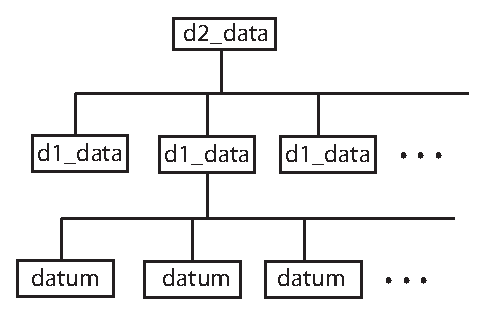
\includegraphics[width=4in]{data-tree.eps}
  \caption[Data tree structure]
{A \vn{d2\_data} structure holds a set of \vn{d1\_data} structures. 
A \vn{d1\_data} structure holds an array of datums.}
  \label{f:data.tree}
\end{figure}

\index{d2_data}\index{d1_data}\index{Data}
The horizontal orbit at a particular BPM is an example of an
individual \vn{datum}.  For ease of manipulation, arrays of datums are
grouped into what is called a \vn{d1_data} structure. Furthermore,
sets of \vn{d1_data} structures are grouped into what is called a
\vn{d2_data} structure.  This is illustrated in
Figure~\ref{f:data.tree}.  For example, a \vn{d2_data} structure for
orbit data could contain two \vn{d1_data} structures --- one
\vn{d1_data} structure for the horizontal orbit data and another
\vn{d1_data} structure for the vertical orbit data. Each datum of,
say, the horizontal orbit \vn{d1_data} structure would then correspond
to the horizontal orbit at some point in the machine.

When issuing \tao commands, all the
data associated with a \vn{d2_data} structure is specified using the
\vn{d2_data} structure's \vn{name}.  The data associated with a
\vn{d1_data} structure is specified using the format
\begin{example}
  d2_name.d1_name
\end{example}
For example, if a \vn{d2_data} structure has the
name ``\vn{orbit}'', and one of its \vn{d1_data} structures has the
name ``\vn{x}'', then \tao commands that refer to the data in this
\vn{d1_data} structure use the name ``\vn{orbit.x}''. Sometimes there
is only one \vn{d1_data} structure for a given \vn{d2_data}
structure. In this case the data can be referred to simply by using
the \vn{d2_data} structure's name. The individual datums can be
referred to using the notation
\begin{example}
  d2_name.d1_name[datum_index]
\end{example}
For example, \vn{orbit.x[10]} referrs to the horizontal orbit datum
with index 10. Notice that the beginning (lowest) datum index is user
selectable and is therefore not necessarily 1.

Ranges of datams can be referred to using using a comma \vn{,} to
separate the indexes combined with the notaion \vn{n1:n2} to specify
all the datums between \vn{n1} and \vn{n2} inclusive. For example
\begin{example}
  orbit.x[3:6,23]
\end{example}
refers to datums 3, 4, 5, 6, and 23. 

If multiple universes (\sref{s:universe}) are present, then the prefix
\vn{n@} signifies the n\Th universe. For example
\begin{example}
  2@orbit.x
\end{example}
would refer to the \vn{orbit.x} data in universe 2. When not
specified, the current ``viewed'' universe is assumed. The current
\vn{viewed} universe has index \vn{0} so \vn{orbit.x} is
equivalent to \vn{0@orbit.x}.

As explained in Section~\sref{s:data.anatomy}, each individual datum
has a number of components. The syntax to refer to a component is:
\begin{example}
  d2_name.d1_name[datum_index]|component
\end{example}
For example:
\begin{example}
  orbit.x[3:10]|meas     ! The measured data values
\end{example}

In referring to datums, a ``\vn{*}'' can be used as a wild card to 
denote ``all''. Thus:
\begin{example}
  *@orbit.x       ! The \vn{orbit.x} data in all universes.
  *               ! All the data in the currently viewed universe.
  *.*             ! Same as *
  *@*             ! All the data in all the universes. 
  *@*.*           ! Same as *@*
  orbit.x[*]|meas ! All measured values of orbit.x
  orbit.x|meas    ! Same as orbit.x[*]|meas
\end{example}
The last example shows that when referring to an entire block of data
encomposed by a \vn{d1_data} structure, the \vn{[*]} can be omitted.

%------------------------------------------------------------------------
\section{Anatomy of a Datum}
\label{s:data.anatomy}

Each datum has a number of quantities associated with it:
\begin{example}
  ele_name       ! Character: Corresponding lattice element name.
  ele0_name      ! Character: Name of range marker element.
  data_type      ! Character: Type of data: "orbit.x", etc.
  merit_type     ! Character: Type of constraint: 'target', 'max', etc.
  data_source    ! Character: How the datum is calculated. 'lattice', or 'beam'.
  ix_ele            ! Integer: Index of "ele" in the element list.
  ix_ele0           ! Integer: Index of "ele0" in the element list.
  ix_ele_merit      ! Integer: Lattice index where merit is evaluated.
  ix_d1             ! Integer: Index number in d1_data structure
  ix_data           ! Integer: Index in the global data array
  ix_dModel         ! Integer: Row number in the dModel_dVar derivative matrix.
  ix_bunch          ! Integer: Bunch number to get the data from.
  meas              ! Real: Measured datum value. 
  ref               ! Real: Measured datum value from the reference data set.
  model             ! Real: Datum value as calculated from the model.
  design            ! Real: What the datum value is in the design lattice.
  old               ! Real: The model at some previous time.
  base              ! Real: The value as calculated from the base model.
  fit               ! Real: The value as calculated from a fitting procedure.
  delta_merit       ! Real: Diff used to calculate the merit function term 
  weight            ! Real: Weight for the merit function term
  merit             ! Real: Merit function term value: weight * delta^2
  conversion_factor ! Real: Typically used to convert coupling to cbar
  s                 ! Real: longitudinal position of ele.
  relative          ! Logical: Is this a relative datum?
  exists            ! Logical: Does the datum exist?
  good_model        ! Logical: Does the model cmponent contain a valid value?
  good_meas         ! Logical: Does the meas cmponent contain a valid value?
  good_ref          ! Logical: Does the ref cmponent contain a valid value?
  good_user         ! Logical: Does the user want this datum used in optimization?
  good_opt          ! Logical: Can be used in Tao extensions.
  good_plot         ! Logical: Can be used in Tao extensions.
  useit_plot        ! Logical: Is this datum to be used in plotting?
  useit_opt         ! Logical: Is this datum to be used for optimization?
\end{example}
When running \tao, the \vn{show data}
(\sref{s:show}) command can be used to view the components of a datum. 
The \vn{set} command (\sref{s:set}) can be used to set some of these components.

%------------------------------------------------------------------------
\subsection{Datum values}
\label{s:datum.values}

\index{Data!measured}\index{Data!reference}\index{Data!model}
\index{Data!base}\index{Data!design}
A given datum has six values associated it:
\vspace{-2ex}
\begin{description}
  \vspace{-1ex}
  \item[meas] \Newline 
The value of the datum as obtained from some measurement. This is the
target or limit value that is used when running the optimizer. When
doing lattice design, the measured value corresponds to a constraint
value (\ref{c:opti}).
  \vspace{-1ex}
  \item[ref] \Newline
The reference datum value as obtained from some reference measurement. For example,
a measurement before some variable is varied could be designated as
the \vn{reference}, and the datum taken after the variation could be 
designated the \vn{measrued} datum.
  \vspace{-0.5ex}
  \item[model] \Newline
The value of the datum as calculated from the \vn{model} lattice (\sref{s:lattice}).
  \vspace{-0.5ex}
  \item[design] \Newline
The value of the datum as calculated from the \vn{design} lattice (\sref{s:lattice}).
  \vspace{-0.5ex}
  \item[base] \Newline
The datum value as calculated from the \vn{base} lattice (\sref{s:lattice}).
  \vspace{-0.5ex}
  \item[old] \Newline
A datum value that was saved at some point in \tao's calculations. This value
can be ignored.
\end{description}

%------------------------------------------------------------------------
\subsection{Associated Lattice Elements}
\label{s:datum.lat.elements}

\index{Data!Relative}
Associated with a datum are two lattice elements named
\vn{ele0_name} and \vn{ele_name}. Datums can be divided up into four
classes: Datums in the first class, like the emittance in a curcular
ring, do not have associated lattice elements and their corresponding
element names will be blank. Datums in the second class, like the beta
function at a given point, will only have one associated lattice
element given by \vn{ele_name} and \vn{ele0_name} will be blank.
Datums in the third class are associated with a section of the
lattice. For example, the maximum of the beta function in a lattice
region. In this case the \vn{ele0} element marks the beginning of the
region and \vn{ele} marks the end. The final class of datums, called
\vn{relative} datums, means that the datum value is set by the
difference between the value at the lattice element at \vn{ele0} and
the value at \vn{ele}. The betatron phase advance falls into this
category:
\begin{example}
  value = \(\phi\sb{x}\)(ele) - \(\phi\sb{x}\)(ele0)
\end{example}
If a relative datum has a blank \vn{ele0_name} then \vn{ele0} is taken
to be the beginning element of the lattice which is marker element
with index 0 named \vn{BEGINNING}.

The datum components \vn{ix_ele} and \vn{ix_ele0} are the index of
\vn{ele} and \vn{ele0} in the list of lattice elements.

%------------------------------------------------------------------------
\subsection{Datums in Optimization}
\label{s:datum.opt}

When using optimization to do lattice correction or design
(\sref{c:opti}), Individual datums can be excluded from the process
using the \vn{veto} (\sref{s:veto}), \vn{restore} (\sref{s:restore}),
and \vn{use} (\sref{s:use}) commands. These set the \vn{good_user}
component of a datum. This, combined with the setting \vn{exists},
\vn{good_model}, \vn{good_meas}, \vn{good_ref}, and \vn{good_opt}
determine the setting of \vn{useit_opt} which is the component that
determines if the datum is used in the computation of the merit
function. The settings of everything but \vn{good_user} is determined
by \tao

\vn{exists} is set by \tao to True if the datum exists and False
otherwise. A datum may not exist if the type of datum requires the
designation of an associated element but the \vn{ele_name} component
is blank. For example, a \vn{d1_data} array set up to hold orbit data
may use a numbering scheme that fits the lattice so that , say, datum
number 34 in the array does not correspond to an existing BPM.

\vn{good_model} is set according to whether a datum value can be
computed from the \vn{model} lattice. For example, If a circular
lattice is unstable, the beta function and the closed orbit cannot be
computed.

\vn{good_meas} is set True if the \vn{meas} component value is set in
the data initialization file (\sref{s:init.data}) or is set using the
\vn{set} command (\sref{s:set}). Similarly, \vn{good_ref} is set True
if the \vn{ref} component has been set. \vn{good_ref} only affects the
setting of \vn{useit_opt} if the optimization is using reference data
as set by the global variable \vn{opt_with_ref} (\sref{s:globals}).

Finally \vn{good_opt} is meant for use in custom versions of \tao
(\sref{c:custom.tao}) and is always left True by the standard \tao code.


%------------------------------------------------------------------------
\subsection{Datum Calculations}
\label{s:datum.calc}

Data can also be classified by how it is calculated:
\vspace{-2ex}
\begin{enumerate}
  \item \textbf{Lattice Parameters} \Newline
    For example lattice twiss parameters, coupling and floor position.
  \item \textbf{Single Particle Properties} \Newline
    For example particle orbit, BPM reading and phase advance.
  \item \textbf{Bunch Properties} \Newline
    For example bunch sigmas, emittance and beam twiss parameters.
\end{enumerate}
For a given data type the method used to calculate the datum can vary
depending on the tracking type. For {\it single} particle tracking all
data is found from the lattice parameters except for the orbit
data. For \textit{particle bunch} or \textit{macroparticle bunch}
tracking some of the datums are found from the particle distribution
using the appropriate \bmad routines. For example, with single
particle tracking the beta function is found from the lattice
transport matrix, however, with particle or macroparticle tracking the
beta function is found from the particle distribution using the
formula
\begin{equation}
  \beta_x = \frac{<x^{2}>}{\sqrt{<x^{2}> <x'^{2}> - <x x'>^{2}}}.
\end{equation}
The next section will describe how each predefined data type is
calculated.  Custom data types need not fall into one of the above
catagories and can be any real number as calculated in the appropriate
ook routine.


For datums with \vni{non-relative} \vn{data_types} if there is also an
associated \vni{ele0} element then the \vn{model} value is dependent
upon the \vni{merit_type}. For example, with a \vn{beta.x}
\vn{data_type} the model value is determined by Table~\ref{t:eval2}
where \vn{i} goes from the \vn{ele} index to the \vn{ele0} index.
\begin{table}[ht]
\centering
{\tt
\begin{tabular}{|l|l|l|} \hline
  {\it Merit\_Type}       & {\it Model Value} \\ \hline 
  \vni{abs_max} & $\min |\beta_x(i)|$ \\ \hline 
  \vni{abs_min} & $\min |\beta_x(i)|$ \\ \hline 
  \vni{int_max} &                     \\ \hline
  \vni{int_min} &                     \\ \hline
  \vni{min}     & $\min \beta_x(i)$ \\ \hline 
  \vni{max}     & $\min \beta_x(i)$ \\ \hline 
  \vni{target}  & {\it Error}   \\ \hline 
\end{tabular}
}
\caption{\vn{Model} evaluation.}
\label{t:eval2}
\end{table}

%------------------------------------------------------------------------
\section{Tao Data Types}\index{Data!Data Types}
\label{s:data.types}

Table~\ref{t:data.types} lists the predefined data types in \tao.

\vn{wire} data simulates the measurement of a wire scanner. The angle specified
is the angle of the wire with respect to the horizontal axis. The measurement
then measures the second momment $<uu>$ along an axis which is 90 degrees off of
the wire axis. For example, \vn{wire:90} is a wire scanner oriented in the
vertical direction and measures the second moment of the beam along the
horizontal axis, $<xx>$. The resultant data is not the beam size, but the beam
size squared.

Data types marked \vn{global} do not have any particular elements
associated with them.

Emittance can be calculated in one of two ways. One way is to
calculate it from a tracked beam. The other is from the lattice using
the standard radiation integrals (see the Bmad manual). For a linear
lattice, the emittance varies along the length of the line while for a
circular lattice there is a single emittance number. \vn{emit.a}
and \vn{emit.b} are the standard normal mode emittances. With
beam tracking, there are also \vn{projected emittances} which give an
indication of what the beam looks like if projected onto the $x$ or
$y$ axes:
\begin{equation}
  \eta_x (\mbox{(projected)} = \sqrt{<x^2> <p_x^2> - <x p_x>^2}
\end{equation}
Notice that this does {\emph not} correspond to the standard emittance
definition in one dimension:
\begin{equation}
  \eta_x = \sqrt{<(x - \eta_x \, p_z)^2> <(p_x - \eta'_x \, p_z)^2> - 
  <(x - \eta_x \, p_z) \, (p_x - \eta'_x \, p_z)>^2}
\end{equation}
\vn{emit.x} and \vn{emit.y} are the projected emittances.
Also notice that the projected emittance is sometimes defined using
$x'$ and $y'$ in place of $p_x$ and $p_y$. However, in the vast
majority of cases, this does not appreciably affect the numeric
results.

\index{Data!Calculation Method}
\index{unstable_ring}\index{beta}\index{alpha}\index{eta}\index{eta}
\index{etap}\index{phase}\index{orbit}\index{bpm}\index{wire}\index{spin}
\index{cbar}\index{coupling}\index{floor}\index{r}\index{t}\index{tt}
\index{i5a_e6}\index{i5b_e6}\index{s_position}\index{e_tot}
\index{unstable_ring}\index{emittance}\index{chrom}\index{norm_emittance}
\index{sigma}\index{dpx_dx}\index{dpy_dy}\index{dpz_dz}\index{dpa_da}
\index{dpb_db}
\begin{table}[ht] 
\centering 
{\tt\small
\begin{tabular}{|l|l|l|} \hline
  {\it Data\_Type}              & {\it Description}                  &          \\ \hline 
    alpha.x, alpha.y            & Projected Alpha Function           &          \\ \hline 
    alpha.a, alpha.b, alpha.z   & Normal-Mode Alpha Function         &          \\ \hline 
    e\_tot                      & Beam Total Energy                  &          \\ \hline
    beta.x, beta.y              & Projected Beta Function            &          \\ \hline 
    beta.a, beta.b, beta.z      & Normal-Mode Beta Function          &          \\ \hline 
    bpm.x, bpm.y                & Transverse BPM reading             &          \\ \hline 
    eta.x, eta.y                & Projected Dispersion               &          \\ \hline 
    eta.a, eta.b                & Normal-Mode Dispersion             &          \\ \hline 
    etap.x, etap.y              & Projected Dispersion derivative    &          \\ \hline 
    etap.a, etap.b              & Normal-Mode Dispersion derivative  &          \\ \hline 
    momentum\_compaction        & Momentum compaction factor         & relative \\ \hline
    orbit.x, orbit.y            & Transverse orbit                   &          \\ \hline 
    orbit.p\_x, orbit.p\_y      & Tranverse momenta                  &          \\ \hline 
    orbit.z, orbit.z\_p         & Longitudinal orbit and momenta     &          \\ \hline 
    phase.a, phase.b            & Betatron phase                     & relative \\ \hline 
    phase\_frac\_diff           & Fractional phase difference (x-y)  & relative \\ \hline
    \begin{tabular}{@{}l}     
      spin.polarization, \\ 
      spin.theta, spin.phi 
    \end{tabular} 
                          & Particle spin                      &          \\ \hline 
    \begin{tabular}{@{}l}     
      cbar.11, cbar.12, \\ 
      cbar.21, cbar.22 
    \end{tabular} 
                          & Coupling                          &          \\ \hline 
    \begin{tabular}{@{}l}   
      coupling.11b, coupling.12a, \\ 
      coupling.12b, coupling.22a 
    \end{tabular} 
                          & Coupling                          &          \\ \hline 
    floor.x, floor.y, floor.z
                          & Global (``floor'') position       & relative \\ \hline 
    floor.theta           & Global (``floor'') angle          & relative \\ \hline 
    r.$ij$                & 
                           \begin{tabular}{l}
                             Term in linear transfer map \\
                             $1 \le i,j \le 6$
                           \end{tabular}
                                                              & relative \\ \hline 
    t.$ijk$               & 
                           \begin{tabular}{l}
                             Term in 2\Nd order transfer map \\
                              $1 \le i,j,k \le 6$
                           \end{tabular} 
                                                              & relative \\ \hline 
    tt.$ijklm\ldots$      & 
                           \begin{tabular}{l}
                             Term in n\Th order transfer map \\
                              $1 \le i,j,k,\ldots \le 6$
                           \end{tabular} 
                                                              & relative \\ \hline 
    i5a\_e6, i5b\_e6      & Normalized I5 radiation integral  &          \\ \hline
    s\_position           & longitudinal length constraint    & relative \\ \hline 
    unstable\_ring        & Nonzero if a ring is unstable     & global   \\ \hline
    \begin{tabular}{@{}l}
      emit.x, emit.a \\
      emit.y, emit.b \\
      emit.z \\
    \end{tabular}
                          & Emittance                        & global   \\ \hline
    \begin{tabular}{@{}l}  
      norm\_emit.x, norm\_emit.a \\
      norm\_emit.y, norm\_emit.b \\
      norm\_emit.z \\
    \end{tabular} 
                          & Normalized Beam Emittance         &          \\ \hline 
    \begin{tabular}{@{}l}
      chrom.a, chrom.b  \\
    \end{tabular}
                          & Chromaticity for a ring           & global   \\ \hline
    \begin{tabular}{@{}l}   
      sigma.x, sigma.p\_x \\ 
      sigma.y, sigma.p\_y \\
      sigma.z, sigma.p\_z \\
    \end{tabular} 
                          & Bunch size                        &          \\ \hline 
    \begin{tabular}{@{}l}   
      multi\_turn\_orbit.x, multi\_turn\_orbit.p\_x \\ 
      multi\_turn\_orbit.y, multi\_turn\_orbit.p\_y \\
      multi\_turn\_orbit.z, multi\_turn\_orbit.p\_z \\
    \end{tabular} 
                          & Bunch size                        &          \\ \hline 
    \begin{tabular}{@{}l}  
      dpx\_dx, dpa\_da \\
      dpy\_dy, dpb\_db \\
      dpz\_dz \\
    \end{tabular} 
                          & <x p\_x> / <$x^2$> \& Etc...       &          \\ \hline 
    wire.<angle>                & Wire Scanner with wire angle <angle>
                                                               &          \\ \hline
\end{tabular}
} 
\label{t:data.types}
\caption{Predefined Data Types}
\end{table}

\vfill \break
{\vfill}



\chapter{Optimization}
\label{c:opti}

%------------------------------------------------------------------------
\section{Lattice Corrections}

Examples of lattice corrections include flattening the orbit and
adjusting quadrupoles to correct the measured betatron phase. The
general idea is to vary an appropriate set of \vn{variables} with the
aim of minimizing a merit function \vn{M} that is a measure of how
well \vn{data_model}, the data as calculated from the \vn{model} fits
\vn{data_meas}, the measured data
\Begineq
  {\cal M} \equiv \sum_{i} w_i \,
    (\data\_\model(i) -  \data\_\meas(i))^2 + 
  \sum_{j} w_j \,
    (\var\_\model(j) - \var\_\meas(j))^2
  \label{m1}
\Endeq
\vn{var_model} is the value of a variable in the \vn{model} and
\vn{var_meas} is the value as measured at the time the data was taken
and the sum \vn{j} runs over all variables that are allowed to be
varied to minimize \vn{M}. The second term in the merit function
prevents degeneracies (or near degeneracies) in the problem which
would allow \tao to find solutions where \vn{data_model} matches
\vn{data_measured} with the \vn{var_model} having ``unphysical''
values (values far from \vn{var_meas}. The weights $w_i$ and $w_j$
need to be set depending upon how accurate the measred data is
relative to how accurate the calibrations for measuring the
\vn{var_meas} values are. With the second term in the merit function
the number of constraints (number of terms in the merit function) is
always larger than the number of variables and degeneracies can never
occur. 

The algorithm used to vary the \vn{var_model} variables to minimize
\vn{M} is called an \vn{optimizer}. In \vn{command line mode} the
\vn{run} command is used to invoke an \vn{optimizer}. In \vn{single
mode} the \vn{g} key starts an optimizer and the \vn{.} key stops it.
Running an optimizer is also called ``fitting'' since one is tring to
get the \vn{data_model} to be equal to the \vn{data_meas}. With orbits
this is also called ``flattening'' since one generally wants to end up
with an orbit that is on--axis.

In a correction one wants to change the machine variables so that the
measured data corresponds to the design values \vn{data_design}. Thus
the change in the data that one wants is
\begin{example}
  data_change = data_design - data_meas
\end{example}
Once a fit has been made, and presuming that the \vn{data_model} is
resonably close to the \vn{data_meas} this data change within the
\vn{model} lattice can be accomplished by changing the variables by
\begin{example}
  var_change = var_design - var_model
\end{example}
This assumes the system is linear. For many situations this is true
since typically \vn{var_change} is ``small''. Since the variables have
a measrued value of \vn{var_meas} the value that the variables should
be set to is
\begin{example}
  var_final = var_meas + (var_design - var_model)
\end{example}
Notice that the fitting process is independent of the \vn{design}
lattice. It is only when calculating the corrections to the
variables that the \vn{design} lattice plays a roll. 

Sometimes it is desired to fit to changes in data as opposed to the
absolute value of the data. For example, when closing an orbit bump
knob what is important is the difference in orbits before and after
the bump knob is varied. Designating one of these orbit the
\vn{reference}, the appropriate merit function is
\begin{alignat}{1}
  {\cal M} = &\sum_{i} w_i \,
    \left[ \bigl( \data\_\model(i) - \data\_\design(i) \bigr) - 
      \bigl( \data\_\meas(i) - \data\_\reference(i) \bigr) \right]^2 + \CRNO
  &\sum_{j} w_j \,
    \left[ \bigl( \var\_\model(j) - \var\_\design(j) \bigr) -
     \bigl( \var\_\meas(i) - \var\_\reference(i) \bigr) \right]^2 
  \label{m2}
\end{alignat}
where \vn{data_ref} and \vn{var_ref} refer to the reference
measurement.  This merit function is acceptable if the reference data
is taken with the machine reasonably near the design setup so that
nonlinearities can be ignored. If this is not the case then the
fitting becomes a two step process: The first step is to fit the
\vn{model} to the \vn{reference} data using the merit function of
\Eq{m1}. The \vn{base} lattice is then set equal to the \vn{model}
lattice. The second step is to fit the model using the merit function
\begin{alignat}{1}
  {\cal M} = &\sum_{\data: i} w_i 
    \left[ (\data\_\model(i) - \data\_\base(i)) - 
      (\data\_\meas(i) - \data\_\reference(i)) \right]^2 + \CRNO
  &\sum_{\var: j} w_j 
    \left[ (\var\_\model(j) - \var\_\base(j)) -
     (\var\_\meas(i) - \var\_\reference(i)) \right]^2 
  \label{m3}
\end{alignat}

Control of what data and what variables are to be used in the fitting
process is controlled by the \vn{use}, \vn{veto}, \vn{restore}, and
\vn{clip} commands.

%------------------------------------------------------------------------
\section{Lattice Design}

Lattice design is the process of calculating \vn{variable} strengths
to meet a number of criteria called constraints. For example, one
constraint could be that the beta function in some part of the lattice
not exceed a certain value. In this case we can proceed as was done
for lattice correction and define a merit function to be minimized:
\Begineq
  {\cal M} = \sum_{\mbox{constraints} i} w_i \, C_i^2
\Endeq
The general form of the $C_i$ constraint values is
\Begineq
  C = 
    \begin{cases}
    (\mbox{Model} - \mbox{Target})  & Condition \\
    0                               & Otherwise
    \end{cases}
\Endeq
where \vn{model} is the value as calculated from the \vn{model}
lattice and \vn{target} is some given number. Part of the optimization
process is in deciding what the values should be for the \vn{targets}.
The \vn{condition} needed for a non--zero $C_i$ is dependent upon the
\vn{type} of the constraint. There are five constraint types:
\begin{table}[h]
\centering
{\tt
\begin{tabular}{|l|l|l|} \hline
  {\it Constraint Type}  & $C$ & {\it Condition for non-zero $C$} \\ \hline 
  \vn{target}     & \vn{model} - \vn{target}   & \vn{model} $\ne$ \target     \\ \hline 
  \vn{min}        & \vn{model} - \vn{target}   & \vn{model} $<$ \vn{target}   \\ \hline 
  \vn{max}        & \vn{model} - \vn{target}   & \vn{model} $>$ \vn{target}   \\ \hline 
  \vn{abs_min}    & |\vn{model}| - \vn{target} & |\vn{model}| $<$ \vn{target} \\ \hline 
  \vn{abs_max}    & |\vn{model}| - \vn{target} & |\vn{model}| $>$ \vn{target} \\ \hline 
\end{tabular}
}
\caption{Constraint Type List.}
\label{t:con_type}
\end{table}

Since lattice design and lattice corrections are very similar, \tao
combines the two into one generalized correction process. With \tao
the constraint \vn{model} values are identified with the
\vn{data_model} and the \vn{target} values are identified with the \vn{data_meas}.
The different types of \vn{data} that \tao knows about is called the data's \vn{type}

\begin{table}[h] \centering {\tt
\begin{tabular}{|l|l|l|} \hline
  {\it Constraint/Data Type} & {\it Description}     &          \\ \hline 
    beta:x, beta:y    & Twiss parameter              &          \\ \hline 
    alpha:x, alpha:y  & Twiss parameter              &          \\ \hline 
    eta:x, eta:y      & Dispersion                   &          \\ \hline 
    etap:x, etap:y    & Dispersion derivative        &          \\ \hline 
    phase:x, phase:y  & Betatron phase               & relative \\ \hline 
    orbit:x, orbit:y  & Particle orbit               &          \\ \hline 
    cbar:11, cbar:12, cbar:21, cbar:22 
                      & Coupling                     &          \\ \hline 
    floor:x, floor:y, floor:z
                      & Global (``floor'') position  & relative \\ \hline 
    floor:theta       & Global (``floor'') angle     & relative \\ \hline 
    r56            & Term in linear transfer map     & relative \\ \hline 
    t566           & Term in 2nd order transfer map  & relative \\ \hline 
    s              & Longitudinal length constraint  & relative \\ \hline 
\end{tabular}
} \caption{Constraint List.}  \label{t:cons}
\end{table}

\chapter{Tao Initialization}\index{Initialization}
\label{c:init}

\tao is customized for specific machines and specific calculations
using input files and custom software routines. Writing custom
software is covered in the programmer's guide section. This chapter
covers the input files.

In general, the input files tell \tao:
\begin{example}
  1) What the "standard" variables should be.
  2) What the "standard" data is.
  3) What to plot and where to plot it.
\end{example}

\tao first looks for input files in the current directory and then
looks in a directory pointed to by the environmental variable
\vn{TAO_INIT_DIR}.

Initialization parameters are read in from a file using Fortran
namelist input. Fortran namelist breaks up the input file into
blocks. The first line of a namelist block starts with an ampersand
``\&'' followed by the block identifying name. Variables are assigned
using an equal sign ``='' and the end of the block is denoted by a
slash ``/'' For example:
\begin{example}
  &this_block_name
    var1 = 0.123   ! exclamation marks are used for comments
    var2 = 0.456
  /
\end{example}
Variables that have default values can be omitted from the block.  The
order of the variables inside a block is irrelevant.  In between
namelist blocks all text is ignored. Inside a block comments may be
included by using an exclamation mark ``!''.

Note: string variables are case sensitive.

%-----------------------------------------------------------------
\section{Beginning Initialization}
\index{Initialization!beginning}
\label{s:init_global} 


\index{tao_start}
\index{tao.init}
\index{lattice_file}
\index{data_file}
\index{var_file}
\index{plot_file}
\index{single_mode_file}
\index{startup_file}
\index{n_universes}
\index{startup_single_mode}
The initialization starts with an initialization file named
\vn{tao.init}.  \vn{tao.init} needs to have a \vn{tao_start} namelist
block with the following syntax:
\begin{example}
  &tao_start
    lattice_file      = "<file_name>"  ! Default = this file.
    data_file         = "<file_name>"  ! Default = this file.
    var_file          = "<file_name>"  ! Default = this file.
    plot_file         = "<file_name>"  ! Default = this file.
    single_mode_file  = "<file_name>"  ! Default = this file.
    startup_file      = "<file_name>"  ! Default = "tao.startup"
    n_universes       = <integer>            ! Number of universes. Default = 1.
    init_name      = "<init_name>" !Default = 'Tao"
  /
\end{example}
\vn{n_universes} is the number of universes to be created.  \vn{init_name} is
for naming the initialization. This is useful to distinguish between multiple
initialization files with custom versions of \tao.  The other parameters specify
which files to find the other initialization namelists. The following sections
describe each of these initialization namelists and their locations are listed
in table \ref{t:init_files}.

\index{tao_design_lattice}
\index{tao_params}
\index{tao_coupled_uni_init}
\index{tao_beam_init}
\index{tao_macro_init}
\index{tao_var}
\index{tao_d2_data}
\index{tao_d1_data}
\index{tao_plot_page}
\index{tao_template_plot}
\index{tao_template_graph}
\index{element_shapes}
\index{key_bindings}
\begin{table}[h]
\centering {\tt
\begin{tabular}{|l|l|l|l|} \hline
  {\it Namelist} & {\it File Name} & {\it Initialized here}  & {\it Section} \\ \hline
  \vn{tao_design_lattice}   & \vn{lattice_file} & lattice files       & \ref{s:init_lat}    \\ \hline
  \vn{tao_params}           & 'tao.init' & Global Variables    & \ref{s:globals}     \\ \hline
  \vn{tao_coupled_uni_init} & 'tao.init' & Coupled Universes   & \ref{s:coupled_uni} \\ \hline
  \vn{tao_beam_init}        & 'tao.init' & Particle beam       & \ref{s:beam_init}   \\ \hline
  \vn{tao_macro_init}       & 'tao.init' & Macroparticle beam  & \ref{s:macro_init}  \\ \hline
  \vn{tao_var}              & \vn{var_file}     & Variables           & \ref{s:init_var}    \\ \hline
  \vn{tao_d2_data}          & \vn{data_file}    & Data                & \ref{s:init_data}   \\ \hline
  \vn{tao_d1_data}          & \vn{data_file}    & Data                & \ref{s:init_data}   \\ \hline
  \vn{tao_plot_page}        & \vn{plot_file}    & Plotting            & \ref{s:init_plot}   \\ \hline
  \vn{tao_template_plot}    & \vn{plot_file}    & Plotting            & \ref{s:init_plot}   \\ \hline
  \vn{tao_template_graph}   & \vn{plot_file}    & Plotting            & \ref{s:init_plot}   \\ \hline
  \vn{element_shapes}       & \vn{plot_file}    & Plotting            & \ref{s:init_plot}   \\ \hline
  \vn{key_bindings}         & \vn{single_mode_file} & Single Mode     & \ref{s:init_single}   \\ \hline
\end{tabular}}
\caption{Table of \vn{tao} Initialization Namelists}
\label{t:init_files}
\end{table}


%-----------------------------------------------------------------
\section{Lattice Initialization}\index{Initialization!Lattice}
\label{s:init_lat} 

The \vn{lattice_file} variable in the \vn{tao_start} namelist is the
name of the file with the \vn{tao_design_lattice} namelist that
defines where the lattice input files are. The \vn{tao_design_lattice}
namelist has the form
\index{tao_design_lattice}
\index{design_lattice}
\index{design_lattice!file}
\index{design_lattice!parser}
\begin{example}
  &tao_design_lattice
    taylor_order = <num>
    design_lattice(i)%file = "<lattice_file>"
    design_lattice(i)%parser = "<parser>"
  /
\end{example}
\vn{taylor_order} is the order of the Taylor maps. This will override
the Taylor order set in the lattice files. \vn{i} refers to the
universe index, \vn{<lattice_file>} is the name of an input lattice
file and \vn{<parser>} is the name of the parser to use. Possible
choices for \vn{<parser>} are:
\index{bmad}\index{xsif}\index{digested}
\begin{example}
  bmad      ! For a standard bmad lattice file. This is the default.
  xsif      ! For an xsif lattice file.
  digested  ! For a digested BMAD file.
\end{example}

Example:
\begin{example}
  &tao_design_lattice
    design_lattice(1)%file = "this.lat"          ! Default: Use the bmad parser 
    design_lattice(2)      = "that.lat", "xsif"  ! For universe \#2
  /
\end{example}

%-----------------------------------------------------------------
\section{Initializing Globals}\index{Initialization!Globals}
\label{s:globals} 

Global variables are initialized in the \vn{data_and_var_file} using a
namelist block named \vn{tao_params} The syntax of this block is:
\index{tao_params}\index{n_v1_var_max}\index{n_d2_data_max}
\index{n_data_max}\index{n_var_max}\index{global}\index{bmad_com}
\index{csr_com}
\begin{example}
  &tao_params
    n_v1_var_max  = <integer>   ! number of v1 data structures.
    n_d2_data_max = <integer>   ! number of d2 data structures.
    n_data_max    = <integer>   ! Total number of data points
    n_var_max     = <integer>   ! Total number of variables.
    global        = <tao_global_struct>  ! global parameters
    bmad_com      = <bmad_com_struct> ! Bmad global parameters
    csr_com       = <csr_common_struct>  ! CSR global parameters
  /
\end{example}
Example:
\begin{example}
  &tao_params
    n_v1_var_max  = 5
    n_d2_data_max = 6
    n_data_max    = 2000
    n_var_max     = 2000
    global%optimizer = "lm"  ! Set the default optimizer.
  /
\end{example}
\vn{n_d2_data_max} and \vn{n_v1_var_max} are the maximum number of
\vn{d2_data} and \vn{v1_var} structures needed. \vn{n_data_max} is the
maximum number of datums needed and \vn{n_var_max} is the maximum
total number variables used. 

The \vn{tao_global_struct} structure contains \tao global parameters.
\index{y_axis_plot_dmin}\index{u_view}\index{n_opti_cycles}\index{ix_key_bank}
\index{n_key_table_max}\index{n_lat_layout_label_rows}\index{phase_units}
\index{bunch_to_plot}\index{n_curve_pts}\index{random_seed}\index{n_write_file}
\index{track_type}\index{prompt_string}\index{Optimization!setting the optimizer}
\index{default_key_merit_type}\index{write_file}\index{var_limits_on}
\index{plot_on}\index{auto_scale}\index{opt_with_ref}\index{opt_with_base}
\index{single_mode}\index{init_opt_wrapper}\index{lm_opt_deriv_reinit}
\index{label_lattice_elements}\index{label_keys}\index{derivative_recalc}
\index{lattice_recalc}\index{init_plot_needed}
\index{valid_plot_who}\index{print_command}\index{default_init_file}
\index{current_init_file}\index{var_out_file}\index{opt_var_out_file}
\begin{example}
type tao_global_struct
  real(rp) :: y_axis_plot_dmin = 1e-4    ! Minimum y_max-y_min allowed for a graph.
  real(rp) :: lm_opt_deriv_reinit = -1   ! Reinit derivative matrix cutoff
  real(rp) :: de_lm_step_ratio = 1       ! Scaling for step sizes between DE and LM optimizers.
  integer :: u_view = 1                  ! Which universe we are viewing.
  integer :: n_opti_cycles = 20          ! number of optimization cycles
  integer :: ix_key_bank = 0             ! For single mode.
  integer :: n_key_table_max = 0         ! Maximum key table index.
  integer :: n_lat_layout_label_rows = 1 ! How many rows with a lat_layout
  integer :: phase_units = radians\$     ! Phase units on output.
  integer :: bunch_to_plot = 1           ! Which bunch to plot
  integer :: n_curve_pts = 401           ! Number of points for plotting a smooth curve
  integer :: random_seed = 0             ! use system clock by default
  integer :: n_write_file = 0            ! used for indexing 'show write' files
  character(16) :: track_type = 'single' ! or 'beam', 'csr', or 'macro' 
  character(16) :: prompt_string = 'Tao'
  character(16) :: optimizer = 'de'      ! optimizer to use.
  character(16) :: default_key_merit_type
  character(80) :: write_file = 'tao_show.dat'
  logical :: var_limits_on = .true.      ! Respect the variable limits?
  logical :: plot_on = .true.            ! Do plotting?
  logical :: auto_scale = .false.        ! Automatically scale and x-scale the plots?
  logical :: opt_with_ref = .false.      ! use reference data in optimization?
  logical :: opt_with_base = .false.     ! use base data in optimization?
  logical :: single_mode = .false.
  logical :: optimizer_running 
  logical :: init_opt_wrapper = .true.
  logical :: label_lattice_elements = .true. ! For lat_layout plots
  logical :: label_keys = .true.             ! For lat_layout plots
  logical :: derivative_recalc = .true.      ! Recalc before each optimizer run?
  logical :: lattice_recalc = .true.         ! recalculate the lattice?
  logical :: init_plot_needed = .true.       ! reinitialize plotting?
  character(16) :: valid_plot_who(10)        ! model, base, ref etc...
  character(40) :: print_command = 'awprint'
  character(80) :: default_init_file = 'tao.init'
  character(80) :: current_init_file = 'tao.init'
  character(80) :: var_out_file = 'var#.out'
  character(80) :: opt_var_out_file = 'opt_var#.out'
end type
\end{example}

The \vn{bmad_com_struct} holds bmad global variables. 
\index{radiation_damping_on}
\index{radiation_fluctuations_on}\index{sr_wakes_on}\index{lr_wakes_on}
\begin{example}
  type bmad_com_struct
    real(rp) :: d_orb(6) = 1e-5  ! for the make_mat6_tracking routine
    real(rp) :: max_aperture_limit = 1e3    
    real(rp) :: rel_tolerance = 1e-5
    real(rp) :: abs_tolerance = 1e-8
    integer :: taylor_order = 3              ! 3rd order is default
    logical :: use_liar_lcavity = .false.    ! Liar like tracking?
    logical :: sr_wakes_on = .true.          ! Short range wakefields?
    logical :: lr_wakes_on = .true.          ! Long range wakefields
    logical :: mat6_track_symmetric = .true. ! symmetric offsets
    logical :: auto_bookkeeper = .true.      ! Automatic bookkeeping?
    logical :: radiation_damping_on = .false.       ! Damping toggle.
    logical :: radiation_fluctuations_on = .false.  ! Fluctuations toggle.
    logical :: compute_ref_energy = .true.          ! Enable recomputation?
    logical :: trans_space_charge_on = .false.      ! Space charge switch
    logical :: coherent_synch_rad_on = .false.      ! Longitudinal csr 
    logical :: spin_tracking_on = .true.            ! Do particle spin tracking
  end type
\end{example}

The \vn{csr_common_struct} holds global variables for the coherent
synchrotron radiation calculations.
\begin{example}
  type csr_common_struct
    real(rp) ds_track_step                   ! Tracking step size
    integer n_bin                            ! Number of bins (slices) used
    integer particle_bin_span = 2            ! Longitudinal particle length / bin width
    logical :: lcsr_component_on = .true.    ! Longitudinal csr component
    logical :: lsc_component_on = .true.     ! Longitudinal space charge component
    logical :: tsc_component_on = .true.     ! Transverse space charge component
  end type
\end{example}


%-----------------------------------------------------------------
\section{Initializing Coupled Universes}\index{Initialization!Coupling}
\label{s:coupled_uni}

Universes can be coupled together. This can be useful, for example, to attach a
damping ring a pre-accelerator to a linac. The syntax is as follows:
\index{tao_coupled_uni_init}
\index{coupled}
\index{coupled!from_universe}
\index{coupled!at_element}
\index{coupled!at_ele_index}
\index{coupled!at_s}
\index{coupled!match_to_design}
\begin{example}
  &tao_coupled_uni_init
    ix_universe                = <Integer>         ! Universe index.
    coupled%from_universe   = <universe_number> ! coupled from this universe
    coupled%at_element      = <ele_name>        ! coupled at end of element 
    coupled%at_ele_index    = <ele_index>       ! coupled at end of ele with this index
    coupled%at_s            = <number>          ! coupled at poisiton s 
    coupled%match_to_design = <logical>         ! match optics to design parameters
  /
\end{example}
\vn{ix_universe} refers to the universe to be coupled. Any of
\vn{at_element}, \vn{at_ele_index} or \vn{at_s} must be specified but
not more than one. These refer to the location in the lattice where
the beam/particle is extracted into this universe.  The injection is
always at the beginning of the lattice \vn{i}. Setting
\vn{from_universe} = \vn{i} will not work to make a circular
lattice. This must be set in the lattice file.  If there are more than
one element named \vn{<ele_name>} then the last element named as such
will be used. If \vn{ele_name = "end"} then the end of the injection
lattice will be used as the coupling point. If \vn{universe_number =
0} then universe \vn{i} is not injected into from any other universe

\vn{match_to_design} will set up a coupling element that will match
the design twiss parameters between the two lattices. This is
performed by first finding the design twiss parameters for the
extraction point for the first lattice then by use of a \bmad
\vn{match} element match those twiss parameters to the design
beginning twiss parameters for the second lattice. The matching
element is not inserted into either lattice. Instead, it resides in
the \tao coupling structure and is tracked through separately. Note
that the matching element is not an extraction kicker element. If an
extraction kicker element is needed then it should be added to either
the extraction point of the first lattice or the beginning of the
second lattice.

When using coupled lattices then statements in the lattice file for
the lattice begin injected into that refer to the \vn{BEGINNING}
element are only used when setting up the coupling element, otherwise
the injected particle/beam is used to set up the \vn{BEGINNING}
element. This goes for the \vn{tao_macro_init} namelist in the
initialization file also.

Even if the coupling point is not the end of a lattice the standard lattice
calculations will still be performed through to the end of the
lattice.  A universe can only inject into a universe with a greater
universe index, so for example, universe 3 can inject into 4 or 5 but
not 1 or 2.

Example:
\begin{example}
  &tao_coupled_uni_init
    ix_universe = 1
    coupled%from_universe = 0      ! no injection into this universe
    coupled%at_element    = "none"
  /
  &tao_coupled_uni_init
    ix_universe = 2
    coupled%from_universe = 1      ! inject beam/particle form universe 1
    coupled%at_element    = "end"  ! inject from the end of universe 1
    coupled%match_to_design = T    ! match the design lattice optics
  /
\end{example}

%-----------------------------------------------------------------
\section{Initializing Particle Beams}\index{Initialization!Beams}
\label{s:beam_init}

A particle beam is initialized in the \vn{tao_beam_init} namelist block.
The syntax is as follows:
\index{tao_beam_init}    
\index{ix_universe}
\index{calc_emittance}
\index{beam_init}
\index{beam_init!a_norm_emit}
\index{beam_init!b_norm_emit}
\index{beam_init!dPz_dZ}
\index{beam_init!center}
\index{beam_init!sig_e}
\index{beam_init!sig_z}
\index{beam_init!n_bunch}
\index{beam_init!ds_bunch}
\index{beam_init!n_particle}
\index{beam_init!bunch_charge}
\index{beam_init!renorm_center}
\index{beam_init!renorm_sigma}
\index{beam_init!center_jitter}
\index{beam_init!emitt_jitter}
\index{beam_init!siz_z_jitter}
\index{beam_init!siz_e_jitter}
\index{beam_init!polarization}
\begin{example}
  &tao_beam_init
    ix_universe             = <integer>
    calc_emittance          = <logical>   ! calculate emittance for rings
    beam_init%a_norm_emit   = <number>    ! A-mode emittance
    beam_init%b_norm_emit   = <number>    ! B-mode emittance
    beam_init%dPz_dZ        = <number>    ! Energy-Z correlation
    beam_init%center        = <number>*6  ! Bunch center offset relative to
                                          ! reference particle (BMAD coords)
    beam_init%sig_e         = <number>    ! e_sigma in dE/E0
    beam_init%sig_z         = <number>    ! Z sigma in m
    beam_init%n_bunch       = <integer>   ! Number of bunches
    beam_init%ds_bunch      = <number>    ! distance between bunches (meters)
    beam_init%n_particle    = <number>    ! Number of particles per bunch
    beam_init%bunch_charge  = <number>    ! charge per bunch (Coulombs)
    beam_init%renorm_center = <logical>   ! Default is .true.
    beam_init%renorm_sigma  = <logical>   ! Default is .false.
    beam_init%center_jitter = <number>*6  ! Bunch center rms jitter (meters)
    beam_init%emitt_jitter  = <bumber>*2  ! a and b emittance rms jitter (depsilon/epsilon)
    beam_init%siz_z_jitter  = <number>    ! bunch length rms jitter (dz/z)
    beam_init%siz_e_jitter  = <number>    ! bunch energy spread rms jitter (dE/E)
    beam_ini%spin%polarization = <number> ! spin polarization (1.0 = %100 polarizaed)
    beam_ini%spin%theta     = <number> ! spin orientation  (polar coordinate)
    beam_ini%spin%phi       = <number> ! spin orientation  (polar coordinate)
  /
\end{example}
\vn{ix_universe} refers to the universe index. See \bmad documentation on what
the \vn{beam_init} parameters refer to.  The charge per particle is set to
$\vn{bunch_charge} / \vn{n_particle}$ and is used when calculating wakefield
effects.

The twiss parameters at the beginning of the lattice are used in
initializing the beam distribution.  For circular lattices the twiss
parameters will be found from the closed orbit, and the emittance will
be calculated using the \bmad routine \vn{radiation_integrals} unless
\vn{calc_emittance = F} in which case the emittance specified in the
initialization will be used. The state of \vn{calc_emittance} has no
effect on Linear lattices where the initial emittance must be
specified.

The default is single particle tracking. To turn on particle tracking the
\vn{global%track_type} perameter must be set to 'beam.' This can be placed in
the \vn{tao_params} namelist above, for example,
\begin{example}
  &tao_params
    n_v1_var_max  = 5
    n_d2_data_max = 6
    n_data_max    = 2000
    n_var_max     = 2000
    global%optimizer = "lm"  ! Set the default optimizer.
    global%track_type = 'beam'
  /
\end{example}

%-----------------------------------------------------------------
\section{Initializing Macroparticle Beams}\index{Initialization!Macroparticle Beams}
\label{s:macro_init}

A macroparticle beam is initialized in the \vn{tao_macro_init} namelist block.
The syntax is as follows:
\index{tao_macro_init}
\index{ix_universe}
\index{calc_emittance}
\index{macro_init}
\index{macro_init!x!norm_emit}
\index{macro_init!y!norm_emit}
\index{beam_init!dPz_dZ}
\index{macro_init!center}
\index{macro_init!sig_e}
\index{macro_init!sig_z}
\index{macro_init!sig_e_cut}
\index{macro_init!sig_z_cut}
\index{macro_init!n_bunch}
\index{macro_init!n_slice}
\index{macro_init!n_macro}
\index{macro_init!n_part}
\begin{example}
  &tao_macro_init
    ix_universe             = <Integer>   ! Universe index.
    calc_emittance          = <logical>   ! calculate emittance for rings
    macro_init%x%norm_emit  = <number> 
    macro_init%y%norm_emit  = <number> 
    beam_init%dPz_dZ        = <number>    ! Energy-Z correlation
    macro_init%center       = <number>*6  ! Bunch center offset relative to
                                          ! reference particle (BMAD coords)
    macro_init%sig_e        = <number>    ! e_sigma in eV
    macro_init%sig_z        = <number>    ! Z sigma in m
    macro_init%sig_e_cut    = <number>    ! Energy cut in sigmas
    macro_init%sig_z_cut    = <number>    ! Z cut in sigmas
    macro_init%n_bunch      = <integer>   ! Number of bunches
    macro_init%n_slice      = <integer>   ! Number of slices per bunch
    macro_init%n_macro      = <integer>   ! Number of macroparticles per slice
    macro_init%n_part       = <number>    ! Number of particles per bunch
  /
\end{example}
\vn{ix_universe} refers to the universe index. See \bmad documentation
on what the \vn{macro_init} parameters refer to.

The twiss parameters at the beginning of the lattice are used in
initiating the beam distribution.  For circular lattices the twiss
parameters will be found from the closed orbit, and the emittance will
be calculated using the \bmad routine \vn{radiation_integrals} unless
\vn{calc_emittance = F} in which case the emittance specified in the
initialization will be used. The state of \vn{calc_emittance} has no
effect on Linear lattices where the initial emittance must be
specified.

The default is single particle tracking. To turn on macroparticle
tracking the \vn{global%track_type} perameter must be set to 'macro.'
This can be placed in the \vn{tao_params} namelist above, for example,
\begin{example}
  &tao_params
    n_v1_var_max  = 5
    n_d2_data_max = 6
    n_data_max    = 2000
    n_var_max     = 2000
    global%optimizer = "lm"  ! Set the default optimizer.
    global%track_type = 'macro'
  /
\end{example}

%-----------------------------------------------------------------
\section{Initializing Variables}\index{Initialization!Variables}
\label{s:init_var} 

\vn{Variable}s are initialized using the \vn{tao_var} namelist. The
format for this is
\index{tao_var}
\index{v1_var!name}
\index{default_universe}
\index{default_attribute}
\index{default_weight}
\index{default_step}
\index{default_merit_type}
\index{default_low_lim}
\index{default_high_lim}
\index{ix_min_var}
\index{ix_max_var}
\index{var!name}
\index{var!ele_name}
\index{var!attribute}
\index{var!universe}
\index{var!weight}
\index{var!step}
\index{var!low_lim}
\index{var!high_lim}
\index{var!merit_type}
\index{var!good_user}
\begin{example}
  &tao_var
    v1_var%name        = "<var_array_name>"  ! Variable array name.
    default_universe   = "<integer>"         ! Universe variables belong in.
    default_attribute  = "<attribute_name>"  ! Attribute to control.
    default_weight     = <number>            ! Merit_function weight.
                                             ! default = 0.0
    default_step       = <number>            ! Small step value.
                                             ! default = 0.0
    default_merit_type = "<merit_type>"      ! Sets how the merit is calculated.
                                             ! default = 'limit'
    default_low_lim    = <number>            ! Lower variable value limit. 
                                             ! default = -1e30
    default_high_lim   = <number>            ! Upper variable value limit. 
                                             ! default =  1e30
    ix_min_var         = <integer>           ! Minimum array index.
    ix_max_var         = <integer>           ! Maximum array index.
    var(i)%name        = "<var_name>"        ! Individual variable name.
    var(i)%ele_name    = "<ele_name>"        ! Element to be controlled.
    var(i)%attribute   = "<attrib_name>"     ! Attribute to be controlled.
    var(i)%universe    = "<integer>"         ! Universe to be controlled.
    var(i)%weight      = <number>            ! Merit function weight.
    var(i)%step        = <number>            ! Small step size.
    var(i)%low_lim     = <number>            ! Lower variable value limit
    var(i)%high_lim    = <number>            ! Upper variable value limit
    var(i)%merit_type  = "<merit_type_name>" ! Sets how the merit is calculated.
    var(i)%good_user   = <logical>           ! Good optimization variable?
  /
\end{example}
Example:
\begin{example}
  &tao_var
    v1_var%name      = "v_steer"   ! vertical steerings
    default_universe  = "clone"
    default_attribute = "vkick"     ! vertical kick attribute
    default_weight    = 1e3
    default_step      = 1e-5
    ix_min_var        = 0
    ix_max_var        = 99
    var(0:99)%name      = "0w", "1w", "2w", "  ", "4w", ...
    var(0:99)%ele_name  = "v00w", "v01w", "v02w", "    ", "v04w", ...
  /
\end{example}

A \vn{tao_var} block is needed for each variable array to be defined.
\vn{v1_var%name} is the name of the array to be used with \tao
commands. The \vn{var(i)} array of variables has an index \vn{i} that
runs from \vni{ix_min_var} to \vni{ix_max_var}. Each variable has a name
\vn{var(i)%name} to which it can be refered to in \tao commands.  A
lattice element name \vn{var(i)%ele_name} and the element's attribute
to vary \vn{var(i)%attribute} needs to specified. Not all elements
need to \vn{exist} and the element names of non--existent elements
should be undefined or set to a name with only spaces in it. For those
variables where \vn{var(i)%attribute} is not specified in the namelist
the \vn{default_attribute} will be used.


\vn{var(i)%step} establishes what a ``small'' variation of the
variable is. This is used, for example, by some optimizers when
varying variables. If \vn{var%step(i)} is not given for a
particular variable then the default \vn{default_step} is
used. 

\vn{var(i)%universe} gives the universe that the
lattice element lives in. If \vn{var(i)%universe} is not present 
\vn{default_universe} is used instead. In addition to a number, 
\vn{default_universe} can have values:
\index{gang}\index{clone}
\begin{example}
  "gang"     -- Multiple universe control (default).
  "clone"    -- Make a var array block for each universe.
\end{example}
With both \vn{"gang"} and \vn{"clone"} individual \vn{var(i)%universe}
may not be set in the namelist. \vn{"gang"} means that each variable
will control the given attribute in each universe
simultaneously. \vn{"clone"} means that an array of variables will be
duplicated, one for each universe.  To differentiate variables from
different universes \vn{_u<n>} will be appended to each \vn{v1_var%name}
where \vn{<n>} is the universe number.  For example, if \vn{v1_var%name}
is \vn{quad_k1} then the variable block name for the second universe
will be \vn{quad_k1_u2}. The default if both \vn{default_universe} and
all \vn{var(i)%universe} are not given is for \vn{default_universe} to
be \vn{"gang"}

\vn{var(i)%weight} gives the weight coefficient for the contribution
of a variable to the merit function.  If not present then the default
weight of \vn{default_weight} is used.  \vn{var(i)%low_lim} and
\vn{var(i)%high_lim} give the lower and upper bounds outside of which
the value of a variable should not go. If not present
\vn{default_low_lim} and \vn{default_high_lim} are used. If these are
not present as well then by default
\begin{example}
  low_lim  = -1e30
  high_lim =  1e30
\end{example}
\vn{var(i)%merit_type} determines how the merit contribution is calculated.
Possible values are:
\index{limit}\index{target}
\begin{example}
  "limit"       ! Default
  "target"      
\end{example}
For details on \vn{limit} and \vn{target} constraints see Chapter~\ref{c:opti}
on Optimization.

\tao can search for the elements in the lattice to be associated with
each variable type, Likewise, the names for data points can be
automatically generated by using the syntax:
\index{COUNT}
\begin{example}
  var(0)%name = "COUNT: <name_string>###"
  var(0)%ele_name = "SEARCH: <search_string>"
\end{example}
Where \vn{<name_string>} is used in the generation of the variable
name and the hashes is replaced by the variable number in the series
starting with \vni{ix_min_var} (as an integer whose length is equal to
the number of hashes). \vn{<search_string>} can contain the wildcards
\vn{*} and \vn{%}. For example:
\begin{example}
  &tao_var
    v1_var%name  = "quad_k1"
    default_attribute = "k1"
    ...
    ix_min_var = 1
    var(0)%name = "COUNT: Q_####"
    var(0)%ele_name = "SEARCH: Q*"
  /
\end{example}

This will search for all lattice elements whose names contain 'Q'
followed by any set of characters and will name the data elements as
'Q\_' followed by the variable number in the v1\_var array starting
with 0001.

Variables can also be searched using the \bmad element \textit{key}
attribute using the syntax:

\begin{example}
  var(0)%name = "COUNT: <name_string>###"
  var(0)%ele_name = "SEARCH_KEY: <key>"
\end{example}
Where \vn{<key>} is the \bmad \textit{key} attribute. For example:
\begin{example}
  &tao_var
    v1_var%name  = "quad_k1"
    default_attribute = "k1"
    ...
    ix_min_var = 1
    var(0)%name = "COUNT: Q_####"
    var(0)%ele_name = "SEARCH_KEY: quadrupole"
  /
\end{example}
will search for all quadrupole elements in the lattice.


%-----------------------------------------------------------------
\section{Initializing Data and
Constraints}\index{Initialization!Data}\index{Initialization!Constants}
\label{s:init_data} 

Data is initialized using the \vn{tao_d2_data} namelist block whose format is
\index{tao_d2_data}
\index{d2_data!name}
\index{universe}
\index{default_merit_type}
\index{default_data_noise}
\index{n_d1_data}
\begin{example}
  &tao_d2_data
    d2_data%name = "<d2_name>"    ! d2_data name.
    universe     = <integer>      ! Universe variables belong in.
                                        !   0 => all universes (default).
    default_merit_type = "<merit_type>" ! Sets how the merit is calculated.
    default_data_noise  = <number>       ! RMS noise on data (only some data types)
    n_d1_data          = <integer>      ! Number associated d1_data arrays.
  /
\end{example}
For example:
For example:
\begin{example}
  &tao_d2_data
    d2_data%name = "orbit"
    universe     = 0  ! apply to all universes
    n_d1_data    = 2
  /
\end{example}
A \vn{tao_d2_data} block is needed for each \vn{d2_data} structure
defined. \vn{d2_data%name} gives the name of the structure.
\vn{universe} gives the universe that the data is associated with. A
value of zero means that a \vn{d2_data} structure is set up in each
universe. \vn{default_merit_type} determines how the merit function
terms are calculated for the individual datum points. Possibilities
are:
\index{target}
\index{max}
\index{min}
\index{abs_max}
\index{abs_min}
\begin{example}
  "target"
  "max"
  "min"
  "abs_max"
  "abs_min"
\end{example}
See Chapter~\ref{c:opti} on optimization for more
details.\vni{default_data_noise} gives the RMS noise on \vn{bpm} and \vn{wire} 
data types. All other data types ignore this parameter.

\vn{n_d1_data} defines how many \vn{d1_data} structures are associated
with the \vn{d2_data} structure. For each \vn{n_d1_data} structure
there must be a \vn{tao_d1_data} namelist which has the form:
\index{tao_d1_data}
\index{ix_d1_data}
\index{d1_data!name}
\index{default_data_type}
\index{default_weight}
\index{ix_min_data}
\index{ix_max_data}
\index{data!name}
\index{data!data_type}
\index{data!ele_name}
\index{data!ele0_name}
\index{data!merit_type}
\index{data!meas_value}
\index{data!weight}
\index{data!data_noise}
\index{data!good_user}
\begin{example}
  &tao_d1_data
    ix_d1_data         = <integer>      ! d1_data index
    d1_data%name       = "<d1_name>"    ! d1_data name.
    default_data_type  = <type_name>    ! Eg: orbit.x, beam_energy, etc...
    default_weight     = <number>       ! Merit function weight.
                                        ! default = 0.0
    ix_min_data        = <integer>      ! Minimum array index.
    ix_max_data        = <integer>      ! Maximum array index.
    data(j)%name       = "<data_name>"  ! Data names.
    data(j)%data_type  = "<type_name>"  ! Eg: "orbit.x", etc.
    data(j)%ele_name   = "<ele_name>"   ! Lattice element names.
    data(j)%ele0_name  = "<ele0_name>"  ! Reference lattice element names.
    data(j)%merit_type = "<merit_type>" ! Sets how the merit is calculated.
    data(j)%meas_value = "<number>"     ! Datum "measured" value
    data(j)%weight     = "<weight>"     ! Merit function weight.
    data(j)%data_noise  = <number"      ! RMS data noise
    data(j)%good_user  = Logical        ! Use for optimization and plotting?
  /
\end{example}
For example:
\begin{example}
  &tao_d1_data
    ix_d1_data        = 1 
    d1_data%name      = "x"  
    default_weight    = 1e6
    ix_min_data       = 0
    ix_max_data       = 99
    data(0:)%name     = "0W",      " ", "2W", ...
    data(0:)%ele_name = "DET_00W", " ", "DET_02W", ...
  /
\end{example}
Alternatively, one can specify a datum in a single line. For example:
\begin{example}
  !         name   data_      ele0_     ele_     merit_   meas_    weight good_
  !                  type       name      name     type     value           user
  &tao_d1_data
  data( 1) = ' '   'beta.x'   'Q09_1'   'Q16_1'  'max'      30      0.1     T
  data( 2) = ' '   'phase.y'  'Q09_1'   'Q16_1'  'max'      30      0.1     T
  data( 3) = ' '   'floor.x'  ' '       'end'    'target'    3      0.01    T       
  data( 4) = ' '   'floor.x'  'B1'      'B2'     'target'    3      0.01    T       
  ...
  /
\end{example}

\vn{ix_min_data} and \vn{ix_max_data} give the bounds for the
\vn{data(i)} structure array that is associated with the \vn{d1_data}
structure. \vn{data(:)%name} gives the names of the data points and
\vn{data(:)%ele_name} gives the lattice element names associated with
the data points. 

A range of elements can be specified by giving an \vn{ele0_name} that
is not a blank string. Thus, in the above example, the value of
\vn{data(1)} is the maximum horizontal beta in the range between the
end of element \vn{Q09_1} to the end of element \vn{Q16_1}.  Certain
data types like the betatron \vn{phase} is measured with respect to a
reference point and in the example above \vn{data(2)} is the phase
advance from \vn{Q09_1} to \vn{Q16_1}.  Some data types can be either
relative or absolute as in the above example where the value of
\vn{data(3)} is the \vn{floor.x} position at element \vn{end} and the
value of \vn{data(4)} is the \vn{floor.x} position at element \vn{B2}
relative to element\vn{B1}.

The relative data types are noted in Table~\ref{t:data_types}. With
these relative data types if \vn{ele0_name} is left blank then the
beginning of the lattice is assumed. For the particular case when a
\vn{d1_data} structure has a \vn{d2_data.d1_data} name of \vn{phase.x}
or \vn{phase.y} there is a subtle difference between using a blank
\vn{ele0_name} and specifying \vn{ele0_name} to be \vn{BEGINNING}
which is the name of the first element that is automatically inserted
in all lattices. With a blank \vn{ele0_name} the average phase or
phase difference for all the datums within a \vn{d1_data} array are
set to zero by adding a fixed constant to all the datums. For example,
in Figure~\ref{f:plot_page1}, the average phase in either of the two
bottom plots is zero. This is done since, without a reference point
that defines a zero phase, the overall average phase is arbitrary and
so the overall phase is taken in \tao to be zero. If the
\vn{BEGINNING} element is explicitly chosen as the reference element
then the average phase is not adjusted. This distinction must be kept
in mind when optimizing since it will affect the merit function.

If elements in the \vn{data} array do not exist the
corresponding \vn{var%name} and \vn{data%ele_name} should be left
blank. Lists of names can be reused using the syntax:
\index{SAME:}
\begin{example}
  data(0)%name = "SAME: <d2_name.d1_name>"
  data(0)%ele_name = "SAME: <d2_name.d1_name>"
\end{example}
For example:
\begin{example}
  &tao_d1_data
    ix_d1_data       = 2
    d1_data%name     = "y"  
    ...
    data(0)%name     = "SAME: orbit.x"
    data(0)%ele_name = "SAME: orbit.x"
  /
\end{example}

\tao can search for the elements in the lattice to be associated with 
each data type, Likewise, the names for data points can be automatically
generated by using the syntax:

\index{COUNT}
\begin{example}
  data(0)%name = "COUNT: <name_string>###"
  data(0)%ele_name = "SEARCH: <search_string>"
\end{example}
Where \vn{<name_string>} is used in the generation of the data name and the
hashes is replaced by the data number in the series starting with
\vn{ix_min_data} (as an integer whose length is equal to the number of 
hashes). \vn{<search_string>} can contain the wildcards
\vn{*} and \vn{%}. For example:
\index{SEARCH}
\begin{example}
  &tao_d1_data
    ix_d1_data       = 1
    d1_data%name     = "x"
    ix_min_data      = 1  
    ...
    data(0)%name     = "COUNT: BPM_####"
    data(0)%ele_name = "SEARCH: BPM*"
  /
\end{example}

This will search for all lattice elements whose names contain 'BPM' followed
by any set of characters and will name the data elements as 'BPM\_'
followed by the data number in the d1\_data array starting with 0001. 

Data elements can also be searched using the \bmad element
\textit{key} attribute using the syntax:

\index{SEARCH_KEY}
\begin{example}
  data(0)%name = "COUNT: <name_string>###"
  data(0)%ele_name = "SEARCH_KEY: <key>"
\end{example}
Where \vn{<key>} is the \bmad \textit{key} attribute. For example:
\begin{example}
  &tao_d1_data
    ix_d1_data       = 1
    d1_data%name     = "x"
    ix_min_data      = 1  
    ...
    data(0)%name     = "COUNT: BPM_####"
    data(0)%ele_name = "SEARCH_KEY: monitor"
  /
\end{example}
will search for all monitor elements in the lattice.

\index{data!data_type}
If \vn{data(j)%data_type} is not given, and \vni{default_data_type} is
not specified, then the \vni{d2_data} name and the \vni{d1_data} name
are combined for each datum to form the datum's \vn{type}. Certain
types are recognized by \tao. These are given by
Table~\ref{t:con_type}. Custom data types not specified in this table
must have a corresponding definition in
\vn{tao_hook_load_data_array.f90}. See
Chapter~\ref{c:prog_customizing} for details.

\index{data%weight}
\vn{data(:)%weight} gives the weight coefficient for a variable in the
merit function. If not present then the default weight of
\vni{default_weight} is used. \vn{bpm_noise} gives the RMS bpm noise on
this bpm.  If not present then \vn{default_bpm_noise} is used.

%-----------------------------------------------------------------
\section{Initializing Plotting}\index{Initialization!Plotting}
\label{s:init_plot} 

\subsection{Plot Window}\index{Initialization!Plotting!Plot Window}

\begin{figure}
  \centering
  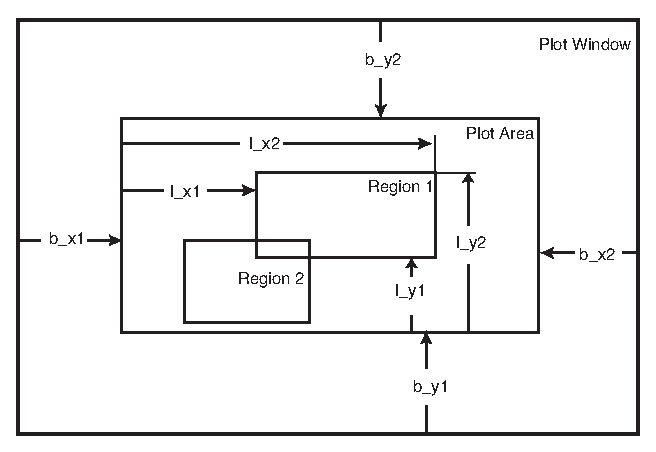
\includegraphics{plot_page.psfig}
  \caption{Regions define where on the plot page plots are placed.}
  \label{f:plot_page}
\end{figure}

Plotting is defined by an initialization file named
\vn{tao_plot.init}.  The first namelist block in the file has a block
name of \vn{tao_plot_page}. This block sets the size of the plot
window (also called the plot page) and defines the ``regions'' where
plots go. The syntax of this block is:
\index{tao_plot_page}    
\index{plot_page!size}
\index{plot_page!border}
\index{plot_page!text_height}
\index{plot_page!title}
\index{region!name}
\index{region!location}
\index{place}
\begin{example}
  &tao_plot_page
    plot_page%size        = <x_size>, <y_size>         ! size in POINTS 
    plot_page%border      = <b_x1>, <b_x2>, <b_y1>, <b_y2>, "<units>"
    plot_page%text_height = <text_height>              !height in POINTS
    plot_page%title(i)    = <string>, {<x>, <y>, "<justify>", "<units>"}
    region(i)%name        = "<region_name>"
    region(i)%location    = <l_x1>, <l_x2>, <l_y1>, <l_y2>  ! % plot area
    place(i)              = "<region>", "<template>"
  /
\end{example}
For example:
\begin{example}
  &tao_plot_page
    plot_page%size        = 700, 800           ! Points
    plot_page%border      = 0, 0, 0, 50, "POINTS"  
    plot_page%text_height = 12.0
    plot_page%title(1)    = "CESR Lattice"
    region(1)%name        = "top"
    region(1)%location    = 0.0, 1.0, 0.5, 1.0
    region(2)%name        = "bottom"
    region(2)%location    = 0.0, 1.0, 0.0, 0.5
    place(1)              = "top", "orbit"
    place(2)              = "bottom", "phase"
  /
\end{example}

\vn{plot_page%size} sets the horizontal and vertical size of the plot
window in \vn{POINTS} units (72 points = 1 inch. Roughly 1 point = 1
pixel). 

\vn{plot_page%border} sets a border around the edges of the
window. As shown in Figure~\ref{f:plot_page} \vn{b_x1}, \vn{b_x2} are
the right and left border widths and \vn{b_y1} and \vn{b_y2} are the
bottom and top border widths respectively.  The rectangle within this
border is called the plot area.

\vn{plot_page%title(i)} set the page title. There are two title areas 
(i = 1,2). If only the title string is given then the other variables 
are set to the defaults \vn{x} = 0.5, \vn{y} = 0.995, \vn{justify} = 
"CC" and \vn{units} = "%PAGE". See the quickplot documentation for 
the \vn{justify} variable syntax.

The plot area is divided up into rectangular regions where plots may
be placed (what defines a plot is discussed below).
\vn{region(i)%name} is the name of a region and my be any character
string. \vn{l_x1}, and \vn{l_x2} define the location of the left and
right edges of the region as a fraction of the plot area width
starting from the left edge of the plot area.  \vn{l_y1} and \vn{l_y2}
define the location of the bottom and top edges of the region as a
fraction of the height of the plot area with respect to the plot
area's bottom edge. Thus, in the above example, region 1 extends from
the left border of the plot area (\vn{region(1)%l_x1} = 0) to the
right border (\vn{region(1)%l_x2} = 0) and vertically from the center
(\vn{region(1)%l_y1} = 0.5) to the top edge (\vn{region(1)%l_x2} =
1.0). Regions may overlap any one can define as many regions as one
likes.

\vn{place(i)} determines the initial placement of plots.

%-----------------------------------------------------------------
\subsection{Templates}\index{Initialization!Plotting!Templates}

As shown in Figure~\ref{f:plot}, a ``plot'' is made up of a collection
of ``graphs'' and a graph consists of axes plus a set of ``curves''.
In the \vn{tao_plot.init} file there needs to be defined a set of
``template plots''. A template plot specifies the layout of a plot:
How the graphs are placed within a plot, what curves are associated
with what graphs, etc. When running \tao, the information in a
template plot may then be transfered to a region using the \vn{place}
command and this will produce a visible plot.

Template plots are defined using namelists with a name of
\vn{tao_template_graph}. The general syntax is:
\index{tao_template_plot}
\index{plot!name}
\index{plot!x}
\index{plot!x_axis_type}
\index{plot!ix_universe}
\index{plot!n_graph}
\index{plot!independent_graphs}
\begin{example}
  &tao_template_plot
    plot%name        = "<plot_name>"
    plot%x           = <qp_axis_struct>
    plot%x_axis_type = "<x_axis_type>"   ! "index" or "s". Default is "index".
    plot%ix_universe = <number> ! used for lat_layout plots
    plot%n_graph     = <n_graphs>
    plot%independent_graphs = <logical>  ! scale graph y-axis independently
  /
\end{example}
For example:
\begin{example}
  &tao_template_plot
    plot%name        = "orbit"
    plot%x%min       =   0
    plot%x%max       = 100
    plot%x%major_div = 10
    plot%x%label     = "Index"
    plot%n_graph     = 2
  /
\end{example}

\vn{plot%x} sets the properties of the horizontal axis. For more
information see the \vn{Quick Plot} documentation on the
\vn{qp_axis_struct}. The major components are
\index{qp_axis_struct!min}
\index{qp_axis_struct!max}
\index{qp_axis_struct!major_div}
\index{qp_axis_struct!minor_div}
\index{qp_axis_struct!label}
\begin{example}
  min        ! Left edge value.
  max        ! Right edge value.
  major_div  ! Number of major divisions. 
             !  Number of major tick marks is one less.
  minor_div  ! Number of minor divisions. 0 = auto choose.
  label      ! Axis label.
\end{example}

\vn{plot%name} is the name that is used with \tao commands to identify
the plot.  

\vn{plot%x_axis_type} sets what is plotted along the
\vn{x-axis}. Possibilities are:
\index{index}
\index{ele_index}
\index{s}
\begin{example}
    "index"      ! Data Index
    "ele_index"  ! Element lattice number index
    "s"          ! Longitudinal position in the lattice.
\end{example}

\vn{n_graph} sets the number of graphs associated with the plot and
each one needs a \vn{tao_template_graph} namelist to define it. These
namelists should be placed directly after their respective
\vn{tao_template_graph} namelists. The general format of the
\vn{tao_template_graph} namelist is:
\index{tao_template_graph}\index{graph!y}\index{curve!name}
\index{graph_index}\index{graph}\index{graph!name}\index{curve}
\index{graph!type}\index{graph!box}\index{graph!title}\index{graph!margin}
\index{graph!y2}\index{graph!n_curve}\index{graph!clip}\index{graph!who}
\index{curve!data_type}\index{curve!data_source}
\index{curve!x_axis_units_factor}\index{curve!y_axis_units_factor}
\index{curve!use_y2}\index{curve!line}\index{curve!ele_ref_name}
\index{curve!draw_line}\index{curve!draw_symbols}\index{curve!ix_universe}
\index{curve!symbol}\index{curve!symbol_every}\index{curve!convert}
\begin{example}
  &tao_template_graph
    graph_index           = <number>
    graph%name            = "<graph_name>"
    graph%type            = "<graph_type>"
    graph%box             = <ix>, <iy>, <ix_tot>, <iy_tot>
    graph%title           = "<label>''
    graph%margin          =  <ix1>, <ix2>, <iy1>, <iy2>, "<Units>"
    graph%y               = <qp_axis_struct>
    graph%y2              = <qp_axis_struct>
    graph%n_curve         = <number_of_curves>
    graph%clip            = <logical> ! Clip plot at grpah boundary. default = .true.
    graph%who(i)          = "<who_to_plot>", <sign>
    curve(i)%name         = "<curve_name>"
    curve(i)%data_type    = "<data_type>"
    curve(i)%data_source  = "<source_name>" !source for the data curve points
    curve(i)%x_axis_scale_factor = <factor> ! scale the x-axis by this.
    curve(i)%y_axis_scale_factor = <factor> ! scale the y-axis by this.
    curve(i)%use_y2       = <logical> 
    curve(i)%draw_line    = <logical>
    curve(i)%draw_symbols = <logical>
    curve(i)%ix_universe  = <universe_number> ! default = 0 => use viewed universe
    curve(i)%line         = <qp_line_struct>
    curve(i)%symbol       = <qp_symbol_struct>
    curve(i)%symbol_every = <integer>       ! plot symbol every # datums
    curve(i)%convert      = <Logical>
    curve(i)%draw_interpolated_curve = <Logical>
    curve(i)%ele_ref_name = "<element_name>"     ! reference element.
  /
\end{example}
For example:
\begin{example}
  &tao_template_graph
    graph_index           = 1
    graph%name            = "x"
    graph%type            = "data"
    graph%box             = 1, 1, 1, 2
    graph%title           = "Horizontal Orbit (mm)"
    graph%margin          =  60, 200, 30, 30, "POINTS"
    graph%y%label         = "X"
    graph%y%max           =  4
    graph%y%min           = -4
    graph%y%major_div     = 4
    graph%n_curve         = 1
    graph%who(1)          = "model", +1
    graph%who(2)          = "design", -1
    curve(1)%data_source  = 'data_array'
    curve(1)%data_type    = "orbit.x"
    curve(1)%units_factor = 1000
    curve(1)%use_y2       = .false.
  /
\end{example}

\vn{graph%name} and \vn{curve%name} define names to be used with
commands. The default names are just the letter \vn{g} or \vn{c} with
the index of the graph or
curve. Thus, in the example above, the name of the curve defaults to
\vn{c1} and it would be referred to as \vn{orbit.x.c1}.

\vn{graph%who(i)} sets what is plotted. In the above example, what will be
plotted is \vn{model - design}. Possible \vn{graph%who}
settings are:
\index{model}\index{design}\index{base}\index{meas}\index{ref}
\begin{example}
  "model"     ! model values.
  "design"    ! design values.
  "base"      ! Base values
  "meas"      ! data values.
  "ref"       ! reference data values.
\end{example}
The default, if \vn{graph%who} is not
specified, is for the graph will show \vn{model} values. 

\vn{graph%type} is the type of graph. \tao knows about the
following types:
\index{data}\index{lat_layout}\index{key_table}\index{phase_space}
\begin{example}
  "data"         ! Data plots (default) 
  "floor_plan"   ! A 2-dimentional birds-eye view of the machine.
  "key_table"    ! Key binding table for single mode.
  "lat_layout"   ! Schematic showing placement of the lattice elements.
  "phase_space"  ! Phase space plots
\end{example}
The \vn{key_table} is drawn with respect to the upper left hand corner
of the region in which it is placed.

\vn{graph%box} sets the layout of the box which the \vn{graph} is
placed in. For a definition of what a box is see the Quick Plot
documentation in the \bmad reference manual. In the above example the
graph divides the region into two vertically stacked boxes and places
itself into the bottom one. 

\index{data_array}\index{var_array}\index{calculation}
\index{curve!data_source}
The \vn{curve} structure is used to define the number and types of
curves to plot in each graph. \vn{curve%data_source} is the type of
information for the source of the data points. There are the following
types of data sources:
\begin{example}
  "data_array"       ! A d1_data array is the source of the curve points.
  "var_array"        ! A v1_var array is the source of the curve points.
  "calculation"      ! The curve points are computed directly from the lattice.
  "beam_calculation" ! The curve points are computed tracking a beam of particles.
\end{example}
With \vn{curve%data_source} set to \vn{data_array}, the values of the
curve points come from the \vn{d1_data} array structure named by
\vn{curve%data_type}. Thus in the above example the curve point values
are obtained from \vn{orbit.x} data. To be valid the data structure
named by \vn{curve%data_type} must be set up in an initialization
file. Similarly, \vn{var_array} indicates that the values of the curve
points come from a \vn{v1_var} array structure. \vn{calculation} means
that the curve data points are calculated from the lattice without
regard to any data structures. \vn{beam_calculation} is used when
tracking beams of particles or macroparticles. In this case the curve
points are calculated from the tracking. For example, with
\vn{curve%data_type} set to \vn{beta.x}, the setting of
\vn{curve%data_source} to \vn{calculation} gives the beta as
calculated from the lattice and \vn{beam_calculation} gives the beta
as calculated from the shape of the beam. 

For a curve with the \vn{curve%data_source} set to \vn{"data_array"} the
possible \vn{curve%data_type} values are the same as the possible
\vn{d1_data%type} values as given in \sref{s:data_types}. If the
\vn{curve%data_source} is \vn{"var_array"} then the possible
\vn{curve%data_type} values are any of the \vn{v1_var} names. This is
what points the curve to the proper data so there needs to be a
corresponding data or var type defined in the initialization file.  If
\vn{graph%type} is \vn{"phase_space"} then \vn{curve%data_source}
determines what planes are plotted. A plane is either:
\index{x}\index{p_x}\index{y}\index{p_y}\index{z}\index{p_z}
\begin{example}
  "x"
  "p_x"
  "y"
  "p_y"
  "z"
  "p_z"
\end{example}
For example:
\begin{example}
  curve%data_type = "x-p_x"  ! x-axis - y-axis
\end{example}
The dash \vn{-} is mandatory as the separator between the plane names. 

\vn{curve%convert} is a logical that is only used
with \vn{curve%data_name} = "coupling" and tells \tao to convert the
coupling data into cbar data before plotting.

\vn{curve%draw_symbols} determines whether a symbol is drawn at the
data points. The size, shape and color of the symbols is determined by
\vn{curve%symbol}.

\vn{curve%draw_line} determines whether a curve is drawn through the
data points. The thickness, style (solid, dashed, etc.), and color
is determined by \vn{curve%line}

%-----------------------------------------------------------------
\subsection{Lattice Layout}\index{Initialization!Lattice Layout}

A lattice layout template plot may be defined that draws the lattice
along a straight line with figures for the various elements.
The \vn{tao_template_plot} needed to define a lattice layout looks like:
\index{tao_template_plot}\index{plot!name}\index{plot!box_layout}
\index{plot!x!min}\index{plot!x!max}\index{plot!n_graph}
\index{tao_template_graph}\index{graph_index}\index{graph!name}
\index{graph!type}\index{graph!title}\index{graph!box}
\index{graph!ix_universe}\index{graph!margin}\index{graph!n_curve}
\begin{example}
  &tao_template_plot
    plot%name        = "<plot_name>"
    plot%box_layout  = <ix>, <iy> 
    plot%x%min       = <number>
    plot%x%max       = <number>
    plot%n_graph     = <number>
  /
  &tao_template_graph
    graph_index       = <number>
    graph%name        = <name>
    graph%type        = "lat_layout"
    graph%title       = "Layout Title"
    graph%box         = <ix>, <iy>
    graph%ix_universe = <integer> ! 0 => use currently viewd universe
    graph%margin      = <ix1>, <ix2>, <iy1>, <iy2>, "<Units>"
    graph%n_curve     = 0
  /
\end{example}
Example:
\begin{example}
  &tao_template_plot
    plot%name       = 'layout'
    plot%x%min      =   0
    plot%x%max      = 100
    plot%n_graph    = 1
  /

  &tao_template_graph
    graph_index       = 1
    graph%name        = 'u1'
    graph%type        = 'lat_layout'
    graph%this_box    = 1, 1
    graph%ix_universe = 1
    graph%margin      = 0.12, 0.12, 0.12, 0.12, '%BOX'
    graph%n_curve     = 0
  /
\end{example}

\index{element_shapes}
\index{shape}
With a \vn{graph%type} of \vn{lat_layout} or \vn{floor_plan}, 
the shapes to be drawn for the various lattice elements need to
be defined using an \vn{element_shapes} namelist whose syntax is:
\begin{example}
  &element_shapes 
    shape(i) = "<key>", "<name>", "<shape>", "<color>", 
                                      "<v_size>", "<print_Label>"
  /
\end{example}
For Example:                 
\begin{example}
  &element_shapes
    shape(1) = "Quadrupole", "Q*",      "Box",  "Red",      30,   T 
    shape(2) = "Quadrupole", "*",       "XBox", "Red",      30,   F 
    shape(3) = "SBend",      "*",       "Box",  "Blue",     15 
    shape(4) = "Wiggler",    "*",       "XBox", "Green",    20 
  /
\end{example}

A figure is drawn for each element in the lattice that matches a
shape. A Match is made if the type of element matches the shape
\vn{<key>} and the name of the element matches the shape
\vn{<name>}. The wildcard ``*'' may be used to denote any number of
characters. Thus, in the example above, \vn{shape(1)} will match to
all quadrupoles whose name begins with ``Q'' and \vn{shape(2)} will
match all quadrupoles. If an element matches more than one shape the
first shape matched will be used. \vn{<shape>} is the shape of the
figure drawn. Valid Shapes are:
\index{box}\index{xbox}
\begin{example}
  "BOX"             -- Rectangular box
  "XBOX"            -- Rectangular box with an x through it.
  "VAR_BOX"         -- Rectangular box with variable height. 
                        The box is symmetric about the center line.
  "ASYM_VAR_BOX"    -- Like VAR_BOX but is not symmetric about the center line. 
\end{example}
The height of a \vn{VAR_HEIGHT_BOX} is proportional to the element
strength. For example, for a quadrupole the height is proportional to
the \vn{K1} focusing strength. Not all elements can be used with a
\vn{VAR_HEIGHT_BOX}.

\vn{<color>} is the color of the shape. Good colors to use are:
\index{black}\index{Red}\index{orange}\index{magenta}\index{yellow}
\index{green}\index{cyan}\index{blue}\index{purple}
\begin{example}
  "BLACK"
  "RED"
  "ORANGE"
  "MAGENTA"
  "YELLOW"
  "GREEN"
  "CYAN"
  "BLUE"
  "PURPLE"
\end{example}
\vn{<v_size} is the vertical size of the shape in points (72 points =
1 inch). Finally \vn{<print_label>} is a logical indicating whether
the element name is to be printed underneath the figure.



%-----------------------------------------------------------------
\section{Initializing Key Bindings for Single Mode}\index{Initialization!Key Bindings}
\label{s:init_single} 

For single mode the bindings of variables to keys is defined with a
\vn{key_bindings} namelist. There is a maximum of 500 key bindings.
The syntax is:
\index{key_bindings}
\index{key}
\begin{example}
  &key_bindings
    key(i) = <ele_name> <attrib_name> <delta> <universe> 
          <small_step> <low_lim> <high_lim> <weight> <good_opt> <merit_type>
  /
\end{example}
For example:
\begin{example}
  &key_bindings
  key(1) = "Q1"   "K1"    0.01 "U:*" 1e-5  -10  10  10  T
  key(2) = "DRFT" "L"     0.1  "U:1" 1e-3    0   3   1  F
  key(3) = "Q3"   "TILT"  0.01 "U:2" 1e-5   -1   1   3  T "target"
  /  
\end{example}
For the \vn{i}\Th key \vn{<ele_name>} is the name of a lattice element
in universe \vn{<universe>} and \vn{<attrib_name>} is the attribute to
be varied. If \vn{<universe>} is ``0'' then the key will vary elements
in all universes. \vn{<delta>} is the change in value when the
appropriate key is depressed. \vn{<small_step>} establishes what a 
``small'' variation of the variable is. 

\vn{merit_type} sets the variable merit is calculated. See
\sref{s:init_var} for more details. the \vn{global%default_key_merit_type} 
sets the default \vn{merit_type}.

If \vn{merit_type} is \vn{"limit"} then \vn{<low_lim>} and
\vn{<high_lim>} establish limits and if the value of the variable goes
outside these limits then the contribution to the merit function is
given by
\index{merit function}
\begin{example}
  merit = <weight> * (var_value - <high_lim>)^2  ! For var_value > <high_lim>
  merit = <weight> * (<low_lim> - var_value)^2   ! Fro <low_lim> > var_value
\end{example}

%---------------------------------------------------------------------------------------------------------------
%---------------------------------------------------------------------------------------------------------------
% WARNING! If you are modifying this file, be aware that the online help system depends upon the lines starting 
% with "%%" to match blocks of text in this file with a given command. 
%
% The online help system also makes some further assumptions about how this file is formatted.
% Please test any modifications by running Tao and using the appropriate help command to see how
% your modifications translate. 
% Note: The translation code is at: 
%     tao/code/tao_help.f90
%---------------------------------------------------------------------------------------------------------------
%---------------------------------------------------------------------------------------------------------------

\chapter{Commands}
\label{c:command}
\index{commands!Command list} 

\tao has two \vn{modes} for entering commands. In \vn{line mode}'', described in this chapter, \tao
waits until the \vn{return} key is depressed to execute a command. That is, a command consists of a
single line of input. Conversely, \vn{Single Mode}, which is described in \vn{Single Mode} chapter
(\sref{c:single}), interprets each keystroke as a command. Single Mode is useful for quickly varying
parameters to see how they affect a lattice but the number of commands in Single Mode is limited. To
put \tao into \vn{single mode} use the \vn{single_mode} command (\sref{s:sing}).

The syntax for \vn{line mode} commands is discussed in Section~\sref{s:com.syntax}. The list of
commands is shown in Table~\ref{t:commands}.

This chapter uses the following special characters to define the command line syntax:
\begin{example}
  \{\}        ! Identifies an optional argument.
            !   Arguments now enclosed in brackets are required
  <>        ! Indicates a non-literal argument.
\end{example}

Example:
\begin{example}
  change \{-silent\} variable <name>[<locations>] <number>
\end{example}
Here the \vn{-silent} argument is optional while the \vn{variable} argument is mandatory.
Appropriate values for \vn{<name>}, \vn{<locations>}, and \vn{<number>} must be substituted. A
possible

\begin{example}
  change var steering[34:36] @1e-3  ! set the steering strength #34-36 to 0.001
\end{example}

%% command_table -----------------------------------------------------

\begin{table}[h]
\centering {\tt
\begin{tabular}{ll|ll} \toprule
  {\it Command} & {\it Section}     & {\it Command} & {\it Section}     \\ \midrule
  alias         & \sref{s:alias}    & re_execute    & \sref{s:re.exe}   \\
  call          & \sref{s:call}     & read          & \sref{s:read}     \\
  change        & \sref{s:change}   & reinitialize  & \sref{s:reinit}   \\ 
  clear         & \sref{s:clear}    & restore       & \sref{s:restore}  \\ 
  clip          & \sref{s:clip}     & run_optimizer & \sref{s:run}      \\ 
  continue      & \sref{s:continue} & scale         & \sref{s:scale}    \\ 
  create        & \sref{s:create}   & set           & \sref{s:set}      \\  
  cut_ring      & \sref{s:cut.ring} & show          & \sref{s:show}     \\ 
  derivative    & \sref{s:deriv}    & single_mode   & \sref{s:sing}     \\ 
  do, enddo     & \sref{s:do}       & spawn         & \sref{s:spawn}    \\ 
  end_file      & \sref{s:end.file} & taper         & \sref{s:taper}    \\
  exit          & \sref{s:exit}     & timer         & \sref{s:timer}    \\
  flatten       & \sref{s:flatten}  & use           & \sref{s:use}      \\ 
  help          & \sref{s:help}     & veto          & \sref{s:veto}     \\ 
  ls            & \sref{s:ls}       & view          & \sref{s:view}     \\
  pause         & \sref{s:pause}    & wave          & \sref{s:wave}     \\
  pipe          & \sref{s:pipe}     & write         & \sref{s:write}    \\
  place         & \sref{s:place}    & x_axis        & \sref{s:x.axis}   \\ 
  ptc           & \sref{s:ptc}      & x_scale       & \sref{s:x.scale}  \\ 
  python        & \sref{s:python}   & xy_scale      & \sref{s:xy.scale} \\ 
  quit          & \sref{s:quit}     &               &                   \\
\bottomrule 
\end{tabular}}
\caption{Table of \tao commands.}
\label{t:commands}
\end{table}

When running \tao, use the \vn{help} (\sref{s:help}) command to show documentation on any command.
For example, \vn{help plot} will show documentation on the \vn{plot} command.

%% Marker: "help" (with no arguments) will not display anything after this line -----------

\vfil
\break

%% alias --------------------------------------------------------------
\section{alias}\index{commands!alias}
\label{s:alias}

The \vn{alias} command defines command shortcuts. Format:
\begin{example}
  alias \{<alias_name> <string>\}
\end{example}

\vskip 7pt 

\vn{Alias} is like Unix aliases. Using the \vn{alias} command without any arguments
results in a printout of the aliases that have been defined. When using an alias up to 9 arguments
may be substituted in the \vn{<string>}. The i\Th argument is substituted in place of the sub-string
``[[i]]'' or ``[<i>]''.  Arguments that do not have a corresponding ``[[i]]'' or ``[<i>]'' are
placed at the end of \vn{<string>}. The difference between ``[[i]]'' and ``[<i>]'' is that ``[[i]]''
is a required argument while ``[<i>]'' defines an optional argument. For example
\begin{example}
  alias aaa show element [[1]] [[2]]
  alias zzz show element [[1]] [<2>]
\end{example}
This defines ``\vn{aaa}'' as an alias for the \vn{show element} command with two required arguments
while ``\vn{zzz}'' has only one requred argument.

Aliases can be set up for multiple commands using semicolons.

Examples:
\begin{example}
  alias xyzzy plot [[1]] model  ! Define xyzzy
  alias                         ! Show all aliases
  xyzzy top                     ! Use an alias
  plot top model                ! Equivalent to "xyzzy top"
  xyzzy top abc                 ! Equivalent to "plot top model abc"
  alias foo  show uni; show top ! "foo" equivalent to "show uni; show top"
\end{example}
In the above example ``xyzzy'' is the alias for the string ``plot [[1]] model''.  When the
command xyzzy is used ``top'' is substituted for ``[[1]]'' in the string.

%% call --------------------------------------------------------------
\section{call}\index{commands!call}
\label{s:call}

The \vn{call} command opens a command file (\sref{s:command.files}) and executes the commands in
it. Format: 
\vskip 1pt
\begin{example}
  call <filename> \{<arg_list>\}
  call -no_calc \{<arg_list>\}
  call -ptc <filename>
\end{example}

\vskip 1pt 
The \vn{call} command without \vn{-ptc} is for running a set of \tao commands.  Up to 9
arguments may be passed to the command file. The i\Th argument is substituted in place of the string
``[[i]]'' in the file. Nesting of command files (command files calling other command files) is
allowed. There is no limit to the number of nested files.  See the \vn{Command Files and Aliases}
section (\sref{s:command.files}) for more details.

The \vn{call -ptc} command passes the command file to PTC for processing. Previous to such a call,
the command \vn{ptc init} must be issued. This is for PTC wizards only.

If a command file calls another command file, and the name of the second command file has a relative
(as opposed to absolute) path name, \tao will look for the second command file relative to the
directory of the first command file. To have \tao look relative to your current working directory
(where you started \tao), use the prefix \vn{\$PWD/}. For example, to call a command file that is
one level up from your current working directory use
\begin{example}
  call \$PWD/../second.cmd
\end{example}

Command loops can be implemented in a command file. See the documentation on \vn{do/enddo}
(\sref{s:do}) for more details.

The \vn{-no_calc} option is equivalent to putting the following at the beginning of the
command file to speed up execution time:
\begin{example}
  set global lattice_calc_on = F   ! Stop lattice calculations (\sref{s:lat.calc}).
  set global plot_on = F           ! Halt replotting 
or
  set calc off                     ! Same as the two lines above.
\end{example}
When using the \vn{-no_calc} option, at the end of the command file the \vn{lattice_calc_on} and
\vn{plot_on} logicals will be toggled back to their initial values.

To suppress all the output when running a command file use the command:
\begin{example}
  set global quiet = all       ! Suppress everything except errors
  set global quiet = warnings  ! Suppress just warnings.
  set global quiet = off       ! No suppression
\end{example}
Note: if \vn{quiet} is set in a command file, the setting will persist to the end of the file and then
revert to what it was before the command file was run.

Examples:
\begin{example}
    call -no my_cmd_file abc def 
\end{example}
In the above example the argument ``abc'' is substituted for any ``[[1]]'' appearing the
file and ``def'' is substituted for any ``[[2]]''.  \Newline

%% change * --------------------------------------------------------------
\section{change}\index{commands!change}
\label{s:change}

The \vn{change} command changes element attribute values or variable values in the \vn{model}
lattice. Format:
\begin{example}
  change \{-update\} element <element_list> <attribute> \{prefix>\} <number>
  change \{-silent\} variable <name>[<locations>] \{<prefix>\} <number>
  change \{n@\}particle_start <coordinate> \{prefix>\} <number>
  change \{-branch <branch_list>\} \{-listing\} \{-mask <veto_list>\} tune \{dQa\} \{dQb\}
  change \{-branch <branch_list>\} z_tune dQz
\end{example}

\vskip 10pt 
The \vn{change} is used for changing real (as opposed to integer or logical) parameters. Also
consider using the \vn{set} command (\sref{s:set}) which is more general.

If \vn{<prefix>} is not present, \vn{<number>} is added to the existing value
of the attribute or variable. That is:
\begin{example}
  final_model_value = initial_model_value + <number>
\end{example}
If \vn{<prefix>} is present, it may be one of
\begin{example}
  @       final_model_value = <number>
  d       final_model_value = design_value + <number>
  \%       final_model_value = initial_model_value * (1 + <number> / 100)
\end{example}

Element list format (\sref{s:ele.list.format}), without any embedded blanks, is used for
the \vn{<element_list>} argument.

For \vn{change particle_start}, The optional \vn{n@} universe specification (\sref{s:universe}) may
be used to specify the universe or universes to apply the change command to.

For lattices with an open geometry, \vn{change particle_start <coordinate> <number>} can be used to
vary the starting coordinates for single particle tracking. If the \vn{use_particle_start} of the
\vn{beam_init} structure (\sref{s:beam.init}) is set to True, \vn{particle_start} will also vary the
beam centroid and the beam particle spin for tracking. Here \vn{<coordinate>} is one of:
\begin{example}
  x, px, y, py, z, pz, t
\end{example}
For photons, \vn{<coordinate>} may also be:
\begin{example}
  e_photon, field_x, field_y, phase_x, phase_y
\end{example}
For closed lattices only the \vn{pz} component is applicable. For lattices that have an \vn{e_gun}
(which necessarily implies that the lattice has an open geometry), the time \vn{t} coordinate must
be varied instead of \vn{pz}.

For open lattices, \vn{change element beginning <twiss>} can be used to vary the starting Twiss
parameters where \vn{<twiss>} is one of:
\begin{example}
  beta_a, beta_b, alpha_a, alpha_b 
  eta_a, eta_b,etap_a, etap_b    
\end{example}

The \vn{change z_tune} command will vary the longitudinal tune by \vn{<dQz>}. The \vn{<branch_list>}
is used to select which lattice branches the tune is varied in. Each branch listed can have an
optional universe prefix. The default is to vary branch 0 of the current default universe.

The \vn{change tune} command will vary the transverse tunes by \vn{<dQa>} and \vn{<dQb>} and 
the \vn{change z_tune} command will vary the longitudinal tune by \vn{<dQz>}. Units are in radians/2pi
With the \vn{change tune} command, if \vn{<dQa>} or \vn{<dQb>} is not given, the value will
be taken to be zero (that is, no change). The \vn{<branch_list>} is a list of lattice
branches with optional universe prefix, to vary the tunes. The \vn{<veto_list>} of the \vn{-mask}
option gives a list of quadrupoles {\em not} to use for varying the tune. See the \vn{set tune}
(\sref{s:set.tune}) command for more details. The \vn{-listing} option, if present, will, in
addition to the tune change, generate a list of quadrupoles varied along with variation
coefficients.

The \vn{-silent} switch, if present, suppresses the printing of what variables are changed.

The \vn{-update} switch, if present, suppresses \tao from printing error messages if a ``variable
slave value mismatch'' is detected (\sref{s:var.mismatch}). Independent of whether \vn{-update} is
present or not, \tao will fix the mismatch using the changed value to set all of the slave values.

Note: The \vn{change element} command can be used with \vn{ramper} type elements.

Examples:
\begin{example}
  change ele 3@124 x_offset 0.1        ! Offset element #124 in universe 3 by 0.1
  change ele 1,3:5 x_offset 0.1        ! Offset elements 1, 3, 4, and 5 by 0.1
  change ele q* k1 d 1.2e-2            ! Set the k1 strength of all elements starting with
                                       !   the letter "q" relative to the design
  change ele quadrupole::* k1 d 1.2e-2 ! Set the k1 strength of all quadrupole elements.
  change var steering[34:36] @1e-3     ! set the steering strength #34-36 to 0.001
  change var steering[*] \%10           ! vary all steering strengths by 10\%
  change 2@particle_start x @0.001     ! set beginning x position in universe 2 to 1 mm.
  change -mask Q1* tune 0 0.01         ! Change transverse tunes without using quadrupoles
                                       !   whose names start with "Q1".
  change -branch 2@1 z_tune 0.02       ! Change z-tune of branch #1 of universe #2.
\end{example}


%% clear --------------------------------------------------------------
\section{clear}\index{commands!clear}
\label{s:clear}

The \vn{clear} command clears stored spin and orbital Taylor maps from all elements in a lattice
with the exception of \vn{Taylor} elements (which are specified in the lattice file as opposed to
being calculated by \bmad). Format:
\begin{example}
  clear maps
\end{example}

Clearing the Taylor maps may be needed if the maps are in use (for example, with a spin polarization
calculation) and orbit excursions place the calculated orbit outside of the range of validity of the
maps.

%% clip --------------------------------------------------------------
\section{clip}\index{commands!clip}
\label{s:clip}

The \vn{clip} command vetoes data points for plotting and optimizing. That is, the \vn{good_user}
logical of the data associated with the out-of-bound plotted points are set to False.  Format:
\begin{example}
  clip \{-gang\} \{<where> \{<limit1> \{<limit2>\}\}\}
\end{example}

\vskip 10pt Which graphs are clipped is determined by the \vn{<where>} switch. If \vn{<where>} is
not present, all graphs are clipped. If \vn{where} is a plot name, then all the graphs of that plot
are clipped. If \vn{where} is the name of a \vn{d2_data} (for example, \vn{orbit}) or a \vn{d1_data}
(for example, \vn{orbit.x}) structure, then those graphs that display this data are clipped.

The points that are clipped those points whose $y$ values are outside a certain range defined by
\vn{<limit1>} and \vn{<limit2>}. If neither \vn{<limit1>} nor \vn{<limit2>} are present, the clip
range is taken to be outside the graph minimum and maximum $y$--axis values. If only \vn{<limit1>}
is present then the clip range is outside the region from -\vn{<limit1>} to +\vn{<limit1>}. If both
are present than the range is from \vn{<limit1>} to \vn{<limit2>}.

The \vn{-gang} switch is apply a clip to corresponding data in a \vn{d2_data} structure. For example
\begin{example}
  clip -g orbit.x   ! Clips both orbit.x and orbit.y 
\end{example}
Here the \vn{orbit.x} data is clipped and the corresponding data in \vn{orbit.y} is also vetoed. For
example, if datum number 23 in \vn{orbit.x} is clipped, datum number 23 in \vn{orbit.y} will be
vetoed.

Examples:
\begin{example}
  clip top.x -3  7  ! Clip the curves in the x graph in the region named "top".
  clip bottom       ! Clip the graphs in the "bottom" region
  clip -g orbit.x   ! Clip the orbit.x graph and also veto corresponding points
                    ! in other graphs of the orbit plot.
\end{example}

%% create --------------------------------------------------------------
\section{create}\index{commands!create}
\label{s:create}

Format:
\begin{example}
  create data ... ! \sref{s:create.data}
\end{example}

The \vn{create} command constructs various tao objects that would have
otherwise been created in tao initialization. 

% Use the command:
%   help create <subcommand>
% to obtain more information on a particular write subcommand. Example:
%   help create data

%% create data --------------------------------------------------------------

\subsection{create data}
\label{s:create.data}

The \vn{create data} constructs a new \vn{d2_data} and one or more \vn{d1_data} for it.
The primary purpose of this command is to make more data available for design
and optimization in an interactive session; for repeated use, create data using
data initialization namelists (\sref{s:init.data}). The resulting data must be
initialized with the \vn{set data} command (\sref{s:set.data}).

Syntax:
\begin{example}
  create data d2_name d1_name[ix_min:ix_max] ...
\end{example}

You may have as many \vn{d1_name}s as needed.
\vn{ix_min} and \vn{ix_max} must be literal integers, not expressions.

%% cut_ring --------------------------------------------------------------
\section{cut_ring}\index{commands!cut_ring}
\label{s:cut.ring}

Format:
\begin{example}
  cut_ring \{-particle_start\} \{-static\} \{-zero\} 
\end{example}

The \vn{cut_ring} command is used to toggle the geometry of the viewed \vn{model} lattice between
\vn{closed} to \vn{open}.

When the lattice is toggled to an open geometry, the \vn{-particle_start}, \vn{-static} or
\vn{-zero} options can be used to set the starting orbit. In all cases, the starting orbit is set
equal to the setting of \vn{particle_start} where \vn{particle_start} can be set in the lattice file
and/or using \tao's \vn{set particle_start} or \vn{change particle_start} commands. 

With the \vn{-static} option (the default), \vn{particle_start} is set to the same orbit as
currently exists for the closed orbit. The exception is if no closed orbit is found. In this case,
\vn{particle_start} is not modified (same as with the \vn{particle_start} option).

With the \vn{-zero} option, the \vn{particle_start} orbit is set to zero. 

With the \vn{-particle_start} option, the \vn{particle_start} orbit is not modified.

\begin{example}
  cut -zero   ! When lattice geometry is toggled open: zero initial orbit.
\end{example}

%% continue --------------------------------------------------------------
\section{continue}\index{commands!continue}
\label{s:continue}

The \vn{continue} command is used to continue reading of a suspended command file
(\sref{s:command.files}) after a \vn{pause} command (\vn{s:pause}). Format:
\begin{example}
  continue
\end{example}

%% do --------------------------------------------------------------
\section{do/enddo command file looping}\index{commands!do}
\label{s:do}

Command loops can be implemented in a command file files. Format:
\begin{example}
  do <var> = <l_bound>, <u_bound> \{, <incr>\}
    ...   ! use the syntax ``[[<var>]]'' to refer to a variable.
  enddo
\end{example}
Note: ``\vn{enddo}'' is one word and my not be split into two words. Loops can be nested and the
number of levels is not unlimited.

A loop will execute the code in between the \vn{do} and \vn{enddo} lines a certain number of
times. Each time trough the the the integer variable \vn{<var>} will be incremented by \vn{<incr>},
starting at \vn{<l_bound>} and stopping before \vn{<var>} is greater than \vn{<u_bound>}. If
\vn{<incr>} is not present, the increment will be 1. Note: \vn{<l_bound>}, \vn{<u_bound>}, and
\vn{<incr>} must all be integers.

Example:
\begin{example}
  do j = 0, 10, 2
    set particle_start pz = 1e-3 * [[j]]
    ...
  enddo
\end{example}
As shown in the above example, to refer to a loop variable in a command, use the syntax ``[[<var>]]''.

%% end_file --------------------------------------------------------------
\section{end_file} \label{s:end.file}
\index{commands!end_file}

The \vn{end_file} command is used in command files (\sref{s:command.files}) to signal the end of the
file. Everything after an \vn{end_file} command is ignored. An \vn{end_file} command entered at the
command line will simply generate an error message.  Format:
\begin{example}
  end_file
\end{example}

%% exit --------------------------------------------------------------
\section{exit}\index{commands!exit}
\label{s:exit}

The \vn{exit} command exits the program. Same as \vn{Quit}.  Format:
\begin{example}
  exit
\end{example}

%% derivative --------------------------------------------------------------
\section{derivative}\index{commands!derivative}
\label{s:deriv}

The \vn{derivative} command calculates the \vn{dModel_Data/dVar} derivative matrix needed for the
\vn{lm} optimizer.  Format:
\begin{example}
  derivative
\end{example}

%% flatten --------------------------------------------------------------
\section{flatten}\index{commands!flatten}
\label{s:flatten}

The \vn{Flatten} command runs the optimizer to minimize the merit function. This is the same as the
\vn{run_optimizer} command.  See the \vn{run_optimizer} command for more details. Format:
\begin{example}
  flatten \{<optimizer>\}
\end{example}

\vskip 10pt

%% help --------------------------------------------------------------
\section{help}\index{commands!help}
\label{s:help}

The \vn{help} command gives help on \tao commands. Format:
\begin{example}
  help \{<command> \{<subcommand>\}\}
\end{example}

\vskip 10pt
The \vn{help} command without any arguments gives a list of all commands.  Some commands, like
\vn{show}, are so large that help on these commands is divided up by their subcommand.

Examples:
\begin{example}
  help            ! Gives list of commands.
  help run        ! Gives help on the run_optimizer command.
  help show       ! Help on the show command.
  help show alias ! Help on the show alias command.
\end{example}

The \vn{help} command works by parsing the file \vn{\$TAO_DIR/doc/command-list.tex} which is the
LaTeX file for the \vn{Tao Commands} chapter of the \tao manual. For the \vn{help} command to work
properly, the environment variable \vn{TAO_DIR} must be appropriately defined. Generally,
\vn{TAO_DIR} will be defined if the appropriate \bmad setup script has been run. For
``Distributions'', this is the same setup script used to setup a distribution. See your local \bmad
guru for details.

When the \vn{help} command parses the \vn{\$TAO_DIR/doc/command-list.tex} file, LaTeX syntax will be
modified to produce a reasonable looking output on the terminal. This translation is not perfect so
reference should be made to the \tao manual if there is a problem in the translation.

%% ls --------------------------------------------------------------
\section{ls}\index{command!ls}
\label{s:ls}

The \vn{ls} command is the same as the standard UNIX \vn{ls} command to display a list of files and
directories. The standard ls switches are accepted. This is equivalent to the \vn{spawn ls} command.
Format:
\begin{example}
  ls \{switches\}
\end{example}

Example:
\begin{example}
  ls -lrt
\end{example}

%% pause --------------------------------------------------------------
\section{pause}\index{commands!pause}
\label{s:pause}

The \vn{pause} command is used to pause \tao when executing a command file
(\sref{s:command.files}). Format:
\begin{example}
  pause \{<time>\} ! Pause time in seconds.
\end{example}

\vskip 10pt
If \vn{<time>} is not present or zero, \tao will pause until the \vn{CR} key is pressed. Once the
\vn{CR} key is pressed, the command file will be resumed. If \vn{<time>} is negative, \tao will
suspend the command file. Commands can now be issued from the keyboard and the command file will be
resumed when a \vn{continue} command (\sref{s:continue}) is issued. Multiple command files can be
simultaneously suspended.  Thus, while one command file is suspended, a second command file can be
run and this command file too can be suspended. A \vn{continue} command will resume the second
command file and when that command file ends, another \vn{continue} command will be needed to
complete the first suspended command file. Use the \vn{show global} command to see the number of
suspended command files.

Example:
\begin{example}
  pause 1.5    ! Pause for 1.5 seconds.
  pause -1     ! Suspend the command file until a \vn{continue} 
               !   command is issued.
\end{example}

%% pipe -----------------------------------------------------------
\section{pipe}\index{commands!pipe}
\label{s:pipe}

The \vn{pipe} command is like the \vn{show} command in that the \vn{pipe} command prints
information to the terminal. The difference is that the output from the \vn{show} command is meant
for viewing by the user while the output of the \vn{pipe} command is meant for easy
parsing. Format:
\begin{example}
  pipe \{-append <file_name>\} \{-noprint\} <subcommand> <arguments>
  pipe \{-write <file_name>\} \{-noprint\} <subcommand> <arguments>
\end{example}

The \vn{pipe} command has \vn{-append} and \vn{-write} optional arguments which can be used to
write the results to a file. The \vn{pipe -append} command will appended to the output file. The
\vn{pipe -write} command will first erase the contents of the output file. Example:
\begin{example}
  pipe -write d2.dat data_d2    ! Write to file "d2.dat"
\end{example}

The \vn{-noprint} option suppresses printing and is useful when writing large amounts of data to a
file.  The \vn{pipe} command can be used to pass information to a parent process when \tao is run
as a subprocess.  The parent process may be any scripting program like Pipe, Perl, Tcl, etc.  In
particular, see the \vn{Python Interface} chapter (\sref{c:python}) for details on how to run
\tao as a Python subprocess.

In terms of long term maintainability, the advantage of using the \vn{pipe} command in the scripts
over the \vn{show} command comes from the fact that the output syntax of \vn{show} commands can (and
does) change.

Note to programmers: For debugging, the \vn{show internal -pipe} command will show the \vn{c_real}
and \vn{c_integer} arrays.

Possible \vn{<subcommand>} choices are:
\begin{example}
  beam, beam_init, branch1, bunch_comb, bunch_params, bunch1, bmad_com, 
  building_wall_list, building_wall_graph, building_wall_point, 
  building_wall_section, constraints, da_params, da_aperture, 
  data, data_d2_create, data_d2_destroy, data_d_array, data_d1_array,
  data_d2, data_d2_array, data_set_design_value, data_parameter,
  datum_create, datum_has_ele, derivative, ele:ac_kicker, ele:cartesian_map,
  ele:chamber_wall, ele:control_var, ele:cylindrical_map, ele:elec_multipoles,
  ele:floor, ele:gen_grad_map, ele:grid_field, ele:gen_attribs, ele:head, ele:lord_slave, 
  ele:mat6, ele:methods, ele:multipoles, ele:orbit, ele:param, ele:photon, 
  ele:spin_taylor, ele:taylor, ele:twiss, ele:wake, ele:wall3d, em_field, enum,
  evaluate, floor_plan, floor_orbit, global, help, inum, lat_branch_list,
  lat_calc_done, lat_ele_list, lat_list, lat_param_units, matrix, merit, orbit_at_s,
  place_buffer, plot_curve, plot_graph, plot_histogram, plot_lat_layout, plot_line,
  plot_plot_manage, plot_graph_manage, plot_curve_manage, plot_list, plot_symbol,
  plot_transfer, plot1, ptc_com, ring_general, shape_list, shape_manage,
  shape_pattern_list, shape_pattern_manage, shape_pattern_point_manage, shape_set,
  show, species_to_int, species_to_str, spin_invariant, spin_polarization, 
  spin_resonance, super_universe, twiss_at_s, universe, var_v1_create, var_v1_destroy, 
  var_create, var_general, var_v1_array, var_v_array, var, wave
\end{example}

%% place --------------------------------------------------------------
\section{place}\index{commands!place}
\label{s:place}

The \vn{place} command is used to associate a \vn{<template>} plot with a \vn{<region>} and thus
create a visible plot in that region. Format:
\begin{example}
  place \{-no_buffer\} <region> <template>
  place <region> none
  place * none
\end{example}

\vskip 10pt 
If \vn{<region>} is set to ``\vn{*}'' then all regions are selected.

If \vn{<template>} is set to ``\vn{none}'' all selected regions are cleared of plots.

The \vn{-no_buffer} optional switch is used when external plotting is being done (EG with a GUI) and
is not of interest otherwise.

Notice that by using multiple \vn{place} commands a \vn{template} can be associated with more than
one region. For example, if multiple orbit plots are desired.

Examples:
\begin{example}
  place * none     ! Erase all plots.
  place top orbit  ! Place the orbit template in the top region
  place top none   ! Erase any plots in the top region
\end{example}

%% ptc -----------------------------------------------------------
\section{ptc}\index{commands!ptc}
\label{s:ptc}

The \vn{ptc} command is used manipulating PTC layouts associated with Bmad
lattices. Format:
\begin{example}
  ptc init            ! Init associated PTC layout.
  ptc reslice         !
\end{example}

\vskip 10pt 

The \vn{ptc init} command initializes a PTC layout.

The \vn{ptc reslice} command calculates good values for lattice element \vn{num_steps} and \vn{integrator_order}. This
command does not adjust the following elements since the algorithm for the calculation can be problematical when the field
is varying longitudinally within an element:
\begin{example}
  rfcavity, lcavity, crab_cavity
  wiggler, undulator
\end{example}

Also see:
\begin{example}
  call -ptc <file>         ! Run a PTC script
  read ptc                 ! Read a PTC lattice
  write ptc                ! Write a PTC lattice
\end{example}

Examples:
\begin{example}
  ptc init
\end{example}


%% python -----------------------------------------------------------
\section{python}\index{commands!python}
\label{s:python}

\vn{Python} is the old name for the \vn{pipe} command. For backwards compatibility,
the old name is still accepted.

%% quit --------------------------------------------------------------
\section{quit}\index{commands!quit}
\label{s:quit}

\vn{Quit} exits the program. Same as \vn{exit}.
Format:
\begin{example}
  quit
\end{example}

%% re_execute --------------------------------------------------------------
\section{re_execute}
\index{commands!re_execute}
\label{s:re.exe}

The \vn{re_execute} command reruns prior commands.  Format:
\begin{example}
  re_execute <index>   ! Re-execute a command with the given index number.
  re_execute <string>  ! Re-execute last command that begins with <string>.
\end{example}

\vskip 10pt 

Every \tao command entered is recorded in a ``history stack''. These commands can be viewed using
the \vn{show history} command. The \vn{show history} command will also display the index number
associated with each command.

Note: The up and down arrow keys on the keyboard can be used to scroll through the command history
stack.

Examples
\begin{example}
  re_exe 34   ! Re-execute command number 34.
  re_exe set  ! Re-execute last ``set'' command.  
\end{example}

%% read --------------------------------------------------------------
\section{read}\index{commands!read}
\label{s:read}

The \vn{read} command is used to modify the (\bmad) \vn{model} lattice or the associated \vn{PTC}
lattice. Format:
\begin{example}
  read lattice \{-silent\} \{-universes <universe-list>\} <file_name>
  read ptc <file_name>
\end{example}

\vskip 10pt 

With the \vn{read lattice} command, the \vn{model} lattices contained in the universes specified by
\vn{<universe-list>} are modified using a ``secondary lattice'' file.  [See the \bmad manual for the
definition of ``secondary lattice''.] For example, with the appropriate file, the \vn{read} command
can be used to misalign the lattice elements. For the \vn{read lattice} command, the input file must
be in Bmad standard lattice format.

If \vn{-universes} is not present, only the \vn{model} lattice
in the default universe is modified.

If, after the lattice file has been read in, a given \tao variable has slave parameters that have
different values there is a problem. For example, if a \tao variable controls the \vn{k2} value of
sextupoles elements \vn{S1} and \vn{S2}, and if \vn{S1} is set to a different value than \vn{S2},
there is an inconsistency which needs to be corrected. This can be done in a number of ways. For
example, by using the \vn{set ele -update} command or using a further \vn{read lattice} command with
a lattice that corrects the problem.

If desired, the \vn{-silent} switch can be used to suppress error messages about differing \tao
variable slave parameter values.

Note: Due to bookkeeping complications, the number of lattice elements may not be modified. If it is
desired to initiate \tao using both ``primary'' and secondary lattice files, this can be done as
illustrated in \sref{s:init.lat}.

The \vn{read ptc} command reads in a PTC lattice. WARNING: This command is untested. Please contact
David Sagan if you want to use it.

Examples:
\begin{example}
  read lat -uni * lat.bmad   ! Modify model lattice of all universes.
  read lat -uni 2,3 lat.bmad ! Modify model lattice universes 2 and 3.
\end{example}

%% reinitialize -------------------------------------------------------
\section{reinitialize}\index{commands!reinitialize}
\label{s:reinit}

The \vn{reinitialize} command reinitializes various things. Format:
\begin{example}
  reinitialize beam
  reinitialize data
  reinitialize tao \{-clear\} \{command line optional arguments\}
\end{example}

\vskip 10pt 

The \vn{reinitialize beam} command reinitializes the beam at the start of the lattice. That is, a
new random distribution is generated.  Note: This also reinitializes the model data.

\vn{reinitialize data} forces a recalculation of the model data.  Normally, a recalculation is done
automatically when any lattice parameter is changed so this command is generally only useful for
debugging purposes.

\vn{reinitializes tao} reinitializes \tao. This can be useful to reset everything to initial
conditions or to perform analysis with more than one initialization file. See the Command Line
Initialization section (\sref{s:command.line}) for a list of the optional arguments. If an argument
is not set, the \vn{reinitialize} command uses the same argument value that were used in the last
\vn{reinitialize} command, or, if this is the first reinitialization, what was used to start \tao.
Exception: If the \vn{-clear} switch is present, all initialization parameters are set to their
default state before the command line arguments specified in the \vn{reinitialize} command are
parsed. The \vn{-clear} switch, if used, should come before any command line arguments since if
there are command line arguments before the \vn{-clear} switch, these arguments will be cleared.

Examples:
\begin{example}
  reinit tao                         ! Reinit using previous arguments
  reinit tao -init special.init      ! Reinitializes \tao with the initialization file 
                                     !   special.init.
  reinit -clear -start my_start      ! Use default init values except for the start file.                    
\end{example}

%% restore --------------------------------------------------------------
\section{restore}\index{commands!restore}
\label{s:restore}

The \vn{restore} command cancels data or variable vetoes. Format:
\begin{example}
  restore data  <data_name> <locations>
  restore var <var_name> <locations>
\end{example}

\vskip 10pt 

See also the \vn{use} and \vn{veto} commands.

Examples:
\begin{example}
  restore data orbit.x[23,34:56]   ! un-veto orbit.x 23 and 34 through 56.
  restore data orbit.x[23,34:56:2] ! un-veto orbit.x 23 and even data between 34 
                                   !                                          and 56
  restore data *@orbit[34]         ! un-veto orbit data in all universes.
  restore var quad_k1[67]          ! un-veto variable
\end{example}

%% run --------------------------------------------------------------
\section{run_optimizer}\index{commands!run}
\label{s:run}

The \vn{run_optimizer} command runs an optimizer. Format:
\begin{example}
  run_optimizer \{<optimizer>\}
\end{example}

\vskip 10pt 

\index{de!optimizer}\index{lm!optimizer}
If \vn{<optimizer>} is not given then the default optimizer is used.  Use the \vn{show optimizer}
(\sref{s:show.optimizer}) command to see optimizer parameters.  To stop the optimizer before it is
finished press the period ``.''  key. If you want the optimizer to run forever run the optimizer in
\vn{single mode}. Valid optimizers are:
\begin{example}
  custom        ! Used when a custom optimizer has been implemented (\sref{c:custom.tao}).
  de            ! Differential Evolution (good for global optimizations).
  geodesic_lm   ! ``Geodesic'' Levenburg-Marquardt (good for local optimizations).
  lm            ! Levenburg-Marquardt (good for local optimizations).
  lmdif         ! Levenburg-Marquardt (alternative version) (good for local optimizations).
  svd           ! svd optimizer (good for local optimizations).
\end{example}

See the optimization chapter (\sref{c:opti}) for details on how \tao structures optimization and for
more details on the different optimizers.

Examples:
\begin{example}
  run         ! Run the default optimizer
  run de      ! Run the de optimizer
\end{example}

%% scale --------------------------------------------------------------
\section{scale}\index{commands!scale}
\label{s:scale}

The \vn{scale} command scales the vertical axis of a graph or set of graphs.  Format:
\begin{example}
  scale \{-exact\} \{-gang\} \{-include_wall\} \{-nogang\} 
             \{-y\} \{-y2\} \{<where> \{<value1> \{<value2>\}\}\}
\end{example}

Which graphs are scaled is determined by the \vn{<where>} switch. If \vn{<where>} is not present or
\vn{<where>} is \vn{all} then all graphs are scaled. \vn{<where>} can be a plot name or the name of
an individual graph withing a plot.

\vn{scale} adjusts the vertical scale of graphs. If neither \vn{<value1>} nor \vn{<value2>} is
present then an \vn{autoscale} is performed and the scale is adjusted so that all the data points
are within the graph region. If an autoscale is performed upon an entire plot, and if
\vn{plot%autoscale_gang_y} (\sref{s:template}) is True, then the chosen scales will be the same for
all graphs. That is, a single scale is calculated so that all the data of all the graphs is within
the plot region. The affect of \vn{plot%autoscale_gang_y} can be overridden by using the \vn{-gang}
or \vn{-nogang} switches.

If only \vn{<value1>} is present then the scale is taken to be from -\vn{<value1>} to +\vn{<value1>}.
If both are present than the scale is from \vn{<value1>} to \vn{<value2>}.

A graph can have a \vn{y2} (left) axis scale that is separate from the \vn{y} (right) axis.
Normally, the \vn{scale} command will scale both axes.  Scaling of just one of these axes can be
achieved by using the \vn{-y} or \vn{-y2} switches.

How a graph is scaled is determined in part by the setting of the \vn{bounds} parameter in the
\vn{y} and \vn{y2} components of the graph. See \vn{s:quick.plot} for more details. The \vn{-exact}
switch, if present, will set \vn{bounds} to \vn{"EXACT"} which means that \tao will use the min and
max bounds as given by \vn{<value1>} and \vn{<value2>} and not try to find ``nice'' values near the
given ones. If \vn{<value1>} and \vn{<value2>} are not given, and if \vn{bounds} is set to
\vn{"EXACT"}, \tao will set \vn{bounds} to \vn{"GENERAL"}. Note: To set the axis \vn{bounds}
directly, use the \vn{set graph} command.

For scaling \vn{floor_plan} plots where there is a building wall to be drawn, if \vn{-include_wall}
is present and autoscaling is being done, then the plot bounds are extended to include the extent of
the building wall.

Examples:
\begin{example}
  scale top.x -3  7  ! Scale the x graph in the top region
  scale -y2 top.x    ! Scale only the y2 axis of the top.x graph.
  scale bottom       ! Autoscale the graphs of the plot in the bottom region
  scale -include     ! Scale everything and include the extent of any 
                     !   building walls in the calculation of the plot bounds.
\end{example}


%% set --------------------------------------------------------------
\section{set}\index{commands!set}
\label{s:set}

The \vn{set} command is used to set values for data, variables, etc. Subcommands are:
\begin{example}
  set beam \{n@\}<parameter> = <value>                        ! \sref{s:set.beam}
  set beam_init \{n@\}<parameter> = <value>                   ! \sref{s:set.beam.init}
  set bmad_com <parameter> = <value>                        ! \sref{s:set.bmad.com}
  set branch <branch> <parameter> = <value>                 ! \sref{s:set.branch}
  set calculate <on/off>                                    ! \sref{s:set.calc}
  set curve <curve> <parameter> = <value>                   ! \sref{s:set.curve}
  set data <data_name>|<parameter> = <value>                ! \sref{s:set.data}
  set default <parameter> = <value>                         ! \sref{s:set.default}
  set dynamic_aperture \{n@\}<parameter = <value>             ! \sref{s:set.da}
  set element <element_list> <attribute> = <value>          ! \sref{s:set.element}
  set floor_plan <parameter> = <value>                      ! \sref{s:set.floor.plan}
  set geodesic_lm <parameter> = <value>                     ! \sref{s:set.geodesic.lm}
  set global <parameter> = <value>                          ! \sref{s:set.global}
  set graph <graph> <parameter> = <value>                   ! \sref{s:set.graph}
  set key <key> = <command>                                 ! \sref{s:set.key}
  set lat_layout <parameter> = <value>                      ! \sref{s:set.lat.layout}
  set lattice \{n@\}<destination_lat> = <source_lat>          ! \sref{s:set.lattice}
  set opti_de_param <parameter> = <value>                   ! \sref{s:set.opti.de.param}
  set particle_start \{n@\}<coordinate> = <value>             ! \sref{s:set.particle.start}
  set plot <plot> <parameter> = <value>                     ! \sref{s:set.plot}
  set plot_page <parameter> = <value1> \{<value2>\}           ! \sref{s:set.plot.page}
  set ptc_com <parameter> = <value>                         ! \sref{s:set.ptc.com}
  set ran_state = <random_number_generator_state>           ! \sref{s:set.ran.state}
  set region <region> <parameter> = <value>                 ! \sref{s:set.region}
  set space_charge_com <parameter> = <value>                ! \sref{s:set.sc.com}
  set symbolic_number <name> = <value>                      ! \sref{s:set.symbolic}
  set tune <Qa> <Qb>                                        ! \sref{s:set.tune}
  set universe <what_universe> <on/off>                     ! \sref{s:set.universe}
  set universe <what_universe> <calc_name> <on/off>         ! \sref{s:set.universe}
  set variable <var_name>|<parameter> = <value>             ! \sref{s:set.variable}
  set wave <parameter> = <value>                            ! \sref{s:set.wave}
  set z_tune <Qz>                                           ! \sref{s:set.z.tune}
\end{example}

\vskip 10pt 

When running \tao, to see documentation on any of the subcommands, use the \vn{help set
<subcommand>} command. For example, \vn{help set element} will show information on the \vn{set
element} subcommand.

Also see the \vn{change} command (\sref{s:change}). The \vn{change} command is specialized for
varying real parameters while the \vn{set} command is more general.

Note: The \vn{show} command (\sref{s:show}) is able to display the settings of many variables that
can be set by the \vn{set} command.

To apply a set to all data or variable classes use ``*'' in place of \vn{<data_name>} or \vn{var_name}.

To set the prompt color, use the command
\begin{example}
  set global prompt_color = <value>
\end{example}
Where \vn{<value>} may be one of:
\begin{example}
  "BLACK"
  "RED"
  "GREEN"
  "YELLOW"
  "BLUE"
  "MAGENTA"
  "CYAN"
  "GRAY"
  "DEFAULT"       ! Default foreground color
\end{example}

% Use the command:
%   help set <subcommand>
% to obtain more information on a particular set subcommand. Example:
%   help set plot

%% set beam --------------------------------------------------------------

\subsection{set beam}
\label{s:set.beam}

Format:
\begin{example}
  set beam \{n@\}<parameter> = <value>
  set beam \{n@\}beginning = <ele-name>
  set beam \{n@\}add_saved_at = <ele-list>
  set beam \{n@\}subtract_saved_at = <ele-list>
\end{example}

The \vn{set beam} command sets beam parameters such as the initial and final tracking positions.
Use the \vn{show beam} command (\sref{s:show}) to see the current values.

For the \vn{set beam beginning <ele-name>} command, the element specified by \vn{<ele-name>} must be
an element where particle positions of the tracked beam have been stored. With this command, the
initial distribution of the beam at the beginning of the lattice will be set to the distribution at
the indicated element. This is useful to track the beam over many turns.

The \vn{set beam \{n@\}add_saved_at} command adds to the list of elements where the beam
distribution is saved at.

The \vn{set beam \{n@\}subtract_saved_at} command subtracts from the list of elements where the beam
distribution is saved at.

The optional \vn{n@} allows the specification of the universe or universes the set is applied to.
The current default universe (\sref{s:universe}) will be used if no universe is given.

Also see the commands: \vn{set beam_init} and \vn{set particle_start}.

Examples:
\begin{example}
  set beam 2@track_start = q10w  ! Set the tracking start at element Q10W in universe 2.
  set beam saved_at = "Q*, B*"   ! Save beam parameters (sigma matrix, etc.) at elements
                                 !  whose names begin with "Q" or "B".
  set beam add_saved_at = S10    ! Save beam parameters at element "S10" as well.
  set beam beginning = end       ! Set the initial beam distribution equal to the distribution at
                                 !  the lattice element named "end".
\end{example}

%% set beam_init --------------------------------------------------------------

\subsection{set beam_init}
\label{s:set.beam.init}

Format:
\begin{example}
  set beam_init \{n@\}<parameter> = <value>
\end{example}

The \vn{set beam_init} command sets parameters of the \vn{beam_init} structure (\sref{s:beam.init}).
Additionally, the \vn{set beam_init} command can set the parameters (\sref{s:beam.init})
\begin{example}
  track_start  and
  track_end
\end{example}

The optional \vn{n@} allows the specification of the universe or universes the set is applied to.
The current default universe (\sref{s:universe}) will be used if no universe is given.

Use the \vn{show beam} command (\sref{s:show}) to see the current values.

Also see the commands: \vn{set beam} and \vn{set particle_start}.

Examples:
\begin{example}
  set beam_init 3@center(2) = 0.004   ! Set px center of beam for universe 3.
  set beam_init [1,2]@sig_pz = 0.02   ! Set sig_pz for universes 1 and 2.
  set beam_init track_end = q10w      ! Set track_end parameter.
\end{example}

%% set bmad_com --------------------------------------------------------------

\subsection{set bmad_com}
\label{s:set.bmad.com}

Format:
\begin{example}
  set bmad_com <parameter> = <value>
\end{example}

Sets global \bmad parameters. Use the \vn{show global -bmad_com} command to see a list of
\vn{<parameter>}s. See the \bmad manual for information on this structure.

Example:
\begin{example}
  set bmad_com radiation_fluctuations_on = T ! Turn on synchrotron radiation fluctuations.
\end{example}

%% set branch --------------------------------------------------------------

\subsection{set branch}
\label{s:set.branch}

Format:
\begin{example}
  set branch <branch-id> <parameter> = <value>
\end{example}

Sets parameters associated with a lattice branch. The parameters that can be set are:
\begin{example}
  particle                  = <species>   ! Reference particle
  default_tracking_species  = <species>   ! Particle that is tracked.
  geometry                  = open or closed
  live_branch               = T or F
\end{example}
Use the \vn{show branch} command to see lattice branch information. \vn{<branch-id>} may be the
branch index or branch name. \vn{<branch-id>} may also contain an optional \vn{n@} prefix to
specify a particular universe to apply the set to. The default is to only set the current viewed
universe.

Note: When toggling a branch from closed to open the beginning orbit and Twiss parameters will not
change. On the other hand, when toggling a branch from open to closed, the orbit and Twiss
parameters will, in general, shift.

Examples:
\begin{example}
  set branch 2@0 live_branch = F     ! Suppress calculations for branch \# 0 of universe 2.
  set branch a_line geometry = open  ! Open geometry for branch named a_line.
  set branch default_tracking_species = positron
                                     ! Set the tracking species to positron.
\end{example}

%% set calculate --------------------------------------------------------------

\subsection{set calculate}
\label{s:set.calc}

Format:
\begin{example}
  set calculate \{<on/off>\}
\end{example}

Toggles the following on (True) or off (False):
\begin{example}
  global%lattice_calc_on
  global%plot_on
\end{example}

Examples:
\begin{example}
  set calc on    ! Sets lattice calc and plot_on to True
  set calc off   ! Sets lattice calc and plot_on to False
  set calc       ! Toggles lattice_calc and sets plot_on to
                 !  the same value as lattice_calc.
\end{example}

%% set curve --------------------------------------------------------------

\subsection{set curve}
\label{s:set.curve}

Format:
\begin{example}
  set curve <curve> <parameter> = <value>
\end{example}

For \vn{set curve}, the \vn{<parameter>}s that can be set are:
\begin{example}
  ele_ref_name        = <string>  ! Name or index of the reference element. Blank => No ref ele.
  ix_ele_ref          = <integer> ! Same as setting ele_ref_name. -1 => No ref ele.
  component           = <string>  ! \sref{s:curve.comp}
  ix_branch           = <integer> ! Branch index.
  ix_bunch            = <integer> ! Bunch index.
  ix_universe         = <integer> ! Universe index.
  symbol_every        = <integer> ! Symbol skip number.
  y_axis_scale_factor = <integer> ! Scaling of y axis
  draw_line           = <logical> 
  draw_symbols        = <logical> 
  draw_symbol_index   = <logical> 
\end{example}
See the \vn{Plot Templates} section (\sref{s:template}) for a description of these attributes.  Use
the \vn{show curve} (\sref{s:show}) to see the settings of the attributes.

If there are visible plots with the same name as the plot parameter of \vn{<curve>}, a template plot
of the same name is ignored. To set template plot curve(s) in this case, add a ``\vn{T::}'' prefix.

Examples:
\begin{example}
  set curve top.x.c1 ix_universe = 2       ! Set universe number for curve.
  set curve T::orbit.x.c1 ix_universe = 2  ! Set curve in template plot.
\end{example}

%% set data --------------------------------------------------------------

\subsection{set data}
\label{s:set.data}

Format:
\begin{example}
  set data \{-silent\} <data_name>|<component> = <value>
\end{example}
Set datum parameters.

parameters that are computed like the \vn{model} value cannot be set. The list of parameter
that \vn{cannot} be set is:
\begin{example}
  model, base, design, old
  good_model, good_base, good_design
  merit, delta_merit
  invalid, exists
  useit_opt, useit_plot
  ix_d1
\end{example}

The \vn{-silent} switch, if present, prevents \tao from issuing an error message if \tao detects a
malformed datum. This is useful when creating datums from scratch (via \vn{pipe data_d2_create})
or when modifying multiple datum parameters, like a datum's \vn{data_type} and \vn{data_source},
where it is known that the datum will be in a malformed state before the final set.

Examples:
\begin{example}
  set data *|ref = *|meas              ! Set ref data = measured in current universe.
  set data 2@orbit.x|ref = 2@orbit.x|model 
                                       ! Set the ref orbit.x in universe 2 to model.
  set data beta.x[10]|weight = 1e-5    ! Set weight of datum.
  set -silent d[1]|data_type = beta.a  ! Set type_type.
\end{example}

%% set default --------------------------------------------------------------

\subsection{set default}
\label{s:set.default}

Format:
\begin{example}
  set default <parameter> = <value>
\end{example}

The parameters that can be set are:
\begin{example}
  branch            ! See: Lattices section (\sref{s:lattice})
  universe          ! See: Universe section (\sref{s:universe})
\end{example}

Use the \vn{show global} (\sref{s:show}) command to see the current
default values.

Example:
\begin{example}
  set default universe = 3
\end{example}

%% set dynamic_aperture --------------------------------------------------------------

\subsection{set dynamic_aperture}
\label{s:set.da}

Format:
\begin{example}
  set dynamic_aperture \{n@\}<parameter> = <value>
\end{example}

The \vn{set dynamic_aperture} command sets parameters for dynamic aperture simulations
(\sref{s:da.calc}) Also see the \vn{set universe dynamic_aperture} (\sref{s:set.universe}) and
\vn{show dynamic_aperture} (\sref{s:show.da}).

To set the particle energy for the <n>\Th scan use \vn{pz(<n>)}. Use a value less than -1 to remove
the scan.

The optional \vn{n@} prefix allows the specification of the universe or universes the set is applied
to. The current default universe (\sref{s:universe}) will be used if no universe is given.

Examples:
\begin{example}
  set dy 2@n_angle = 20   ! Set number of scan points for universe 2.
  set dy accuracy = 1e-5  ! Set scan scan accuracy
  set dy pz(3) = -0.05    ! Set particle energy for the 3rd scan.
\end{example}

%% set element --------------------------------------------------------------

\subsection{set element}
\label{s:set.element}

Format:
\begin{example}
  set \{-update\} element <element_list> <attribute> = <value>
\end{example}

The \vn{set element} command sets the attributes of an element. Use the \vn{show element}
command to view the attributes of an element.

The \vn{-update} switch, if present, suppresses \tao from printing error messages if a ``variable
slave value mismatch'' is detected (\sref{s:var.mismatch}). Independent of whether \vn{-update} is
present or not, \tao will fix the mismatch using the changed value to set all of the slave values.

Note: \vn{set element} can be used to set \vn{ramper} type elements.

Note: If an element in the \vn{<element_list>} does not specify a universe (or universes),
only the element in the viewed universe is used. See the examples below.

Note: It is also possible to use the \vn{change element} command to change real (as opposed to
logical or integer) attributes.

Examples:
\begin{example}
  set ele rfcav::* is_on = F         ! Turn off all rfcavity elements the viewed universe.
  set ele *@rfcav::* is_on = F       ! Turn off all rfcavity elements in all universes.
  set ele A:B track_method = linear  ! Set tracking_method for all elements between 
                                     !   elements A and B
  set ele q10w k1 = 0.7              ! Set element q10w k1 of the viewed universe.
  set ele Q* k1 = ele::Q*[k1]|design ! Set model to design values.
\end{example}

%% set floor_plan --------------------------------------------------------------

\subsection{set floor_plan}
\label{s:set.floor.plan}

Format:
\begin{example}
  set floor_plan <parameter> = <value>
\end{example}


Sets parameters for \vn{floor_plan} plots (\sref{s:shapes}).  Possible \vn{<parameters>} are:
\begin{example}
  <shape_name>%<shape_parameter>
  draw_beam_chamber_wall
  beam_chamber_wall_scale
\end{example}
Where \vn{<ele_shape_name>} is of the form ``\vn{ele_shape(<n>)}'' where \vn{<n>} is the index of
the \vn{ele_shape} in the \vn{floor_plan_drawing} namelist.  Use ``\vn{show plot -floor_plan}'' to
see the current state of the \vn{floor_plan} parameters

Example:
\begin{example}
  set floor_plan ele_shape(2)%draw = F  ! Veto drawing of ele_shape(2)
  set floor_plan beam_chamber_scale = 0.5
\end{example}

%% set geodesic_lm --------------------------------------------------------------

\subsection{set geodesic_lm}
\label{s:set.geodesic.lm}

Format:
\begin{example}
  set geodesic_lm <parameter> = <value>
\end{example}

For \vn{set geodesic_lm}: The \vn{show optimizer geodesic_lm} command will give a list of
\vn{<parameter>}s.

Example:
\begin{example}
  set geodesic_lm method = 10
\end{example}

%% set global --------------------------------------------------------------

\subsection{set global}
\label{s:set.global}

Format:
\begin{example}
  set global <parameter> = <value>
\end{example}

The \vn{set global} command sets global parameters of \tao. The \vn{show global} command will give
a list of global parameters.

Example:
\begin{example}
  set global n_opti_loops = 30  ! Set number of optimization cycles
  set global rf_on = T          ! Turn on the RF cavities.
\end{example}

%% set graph --------------------------------------------------------------

\subsection{set graph}
\label{s:set.graph}

Format:
\begin{example}
  set graph <graph> <parameter> = <value>
\end{example}

The \vn{set graph} command is used to set parameters of a graph structure (\sref{s:template}).

If the \vn{<graph>} name corresponds to a plot, the set is applied to all the graphs associated with
the plot. If there are visible plots with the same name as the plot parameter of \vn{<graph>}, a
template plot of the same name is ignored. To set template plot graphs(s) in this case, add a
``\vn{T::}'' prefix.

For setting the \vn{parameter} attribute see also the commands:
\begin{example}
  set plot parameter      ! \sref{s:set.plot}
  set curve parameter     ! \sref{s:set.curve}
\end{example}

Example:
\begin{example}
  set graph orbit.x component = model - design  ! Plot orbit (model - design).
  set graph orbit component = model - design    ! Applies to all graphs of orbit plot.
  set graph T::orbit.x component = design       ! Set template plot
  set graph r11 floor_plan%orbit_scale = 100    ! To display an orbit.
  set graph beta y%bounds = "zero_at_end"       ! \sref{s:quick.plot}.
\end{example}

%% set key --------------------------------------------------------------

\subsection{set key}
\label{s:set.key}

Format:
\begin{example}
  set key <key> = <command>
\end{example}

Binds a custom command to a key for use in single mode (\sref{c:single}).  This will override the
default behavior (if there is one) of the key.  The command \vn{default} will reset the key to its
default usage.

Example:
\begin{example}
  set key h = veto var *
  set key j = default
\end{example}


%% set lat_layout --------------------------------------------------------------

\subsection{set lat_layout}
\label{s:set.lat.layout}

Format:
\begin{example}
  set lat_layout <parameter> = <value>
\end{example}

Sets parameters for \vn{lat_layout} plots (\sref{s:shapes}).  Syntax for ``\vn{set lat_layout}'' is
identical to syntax of ``\vn{set floor_plan}''.  See ``\vn{set floor_plan}'' for more details.

Use ``\vn{show plot -lat_layout}'' to see a listing of all shapes. 

Example:
\begin{example}
  set lat_layout ele_shape(2)%draw = F  ! Veto drawing of shape \#2
\end{example}

%% set lattice --------------------------------------------------------------

\subsection{set lattice}
\label{s:set.lattice}

Format:
\begin{example}
  set lattice \{n@\}<destination_lat> = <source_lat>
\end{example}

The \vn{set lattice} command transfers lattice parameters (element strengths, etc., etc.)  from one
lattice (the \vn{source} lattice) to another (the \vn{destination} lattice). Both lattices are
restricted to be from the same universe. The optional \vn{n@} prefix (\sref{s:universe}) of the
destination lattice can be used to specify which universe the lattices are in. If multiple universes
are specified, the corresponding destination lattice will be set to the corresponding source lattice
in each universe. Note: At this time, it is not permitted to transfer parameters between lattices in
different universes.

The destination lattices that can be set are:
\begin{example}
  model      ! Model lattice.
  base       ! Base lattice
\end{example}
The source lattice can be:
\begin{example}
  model       ! model lattice.
  base        ! base lattice.
  design      ! design lattice
\end{example}

Note: \tao variables that control parameters in multiple universes can complicate things. If, for
example, there are two universes, and a \tao variable controls, say, the quadrupole strength of
quadrupoles in both universes, then a ``set lat 2@model = design'' will result in the quadrupole
strengths of those quadrupoles controlled by the variable in universe 1 being changed.

Example:
\begin{example}
  set lattice *@model = design  ! Set the model lattice to the design in 
                                !   all universes.
  set lattice base = model      ! Set the base lattice to the model lattice in 
                                !   the default universe.
\end{example}

%% set opti_de_param --------------------------------------------------------------

\subsection{set opti_de_param}
\label{s:set.opti.de.param}

Format:
\begin{example}
  set opti_de_param <parameter> = <value>
\end{example}

For \vn{set opti_de_param}: The \vn{show global} command will give a list of \vn{<parameter>}s.

Example:
\begin{example}
  set opti_de_param binomial_cross = T  ! Use binomial crossovers 
\end{example}

%% set particle_start --------------------------------------------------------------

\subsection{set particle_start}
\label{s:set.particle.start}

Format:
\begin{example}
  set particle_start \{n@\}<coordinate> = <value>
\end{example}
The \vn{set particle_start} command sets the starting coordinates for single particle tracking for
lattices with an open geometry. If the \vn{use_particle_start} of the \vn{beam_init}
structure (\sref{s:beam.init}) is set to True, \vn{particle_start} will also vary the beam centroid
and beam particle spin for beam tracking.

The optional \vn{n@} universe specification (\sref{s:universe}) may be used to specify the universe
or universes to apply the set command to.

\vn{<coordinate>} is one of:
\begin{example}
  x, px, y, py, z, pz, t
  spin_x, spin_y, spin_z
\end{example}
For photons, \vn{<coordinate>} may also be:
\begin{example}
  field_x, field_y, phase_x, phase_y
  e_photon
\end{example}
The \vn{*} coordinate denotes the phase space vector $(x, p_x, y, p_y, z, p_z)$.  For closed
lattices only the \vn{pz} parameter is applicable. For lattices that have an \vn{e_gun} (which
necessarily implies that the lattice has an open geometry), the time \vn{t} coordinate must be
varied instead of \vn{pz}.

For photons, the photon energy can be set by setting \vn{e_photon} which sets the photon energy in
eV or by setting \vn{pz} which sets the relative difference between the photon energy and the
reference energy:
\begin{example}
  photon_energy = reference_energy * (1 + pz)
\end{example}

To see the values for \vn{particle_start} use the command \vn{show element 0}.

Also see the commands: \vn{set beam} (\sref{s:set.beam}), \vn{set beam_init} (\sref{s:set.beam.init}), 
and \vn{change particle_start} (\sref{s:change}).

Examples:
\begin{example}
  set particle_start 2@x = 0.001         ! Set beginning x position in universe 2 to 1 mm.
  set particle_start field_x = 1         ! Set photon field
  set particle_start spin_y = 0.37       ! Set spin parameter.
\end{example}

%% set plot --------------------------------------------------------------

\subsection{set plot}
\label{s:set.plot}

The \vn{set plot} command set various parameters of a plot. Format:
\begin{example}
  set plot <plot_or_region> <parameter> = <value>
\end{example}

The \vn{<parameters>}s that can be set are:
\begin{example}
  autoscale_x        = <logical>
  autoscale_y        = <logical>
  visible            = <logical>
  component          = <string>    ! Sets curve component \sref{s:curve.comp}
  x%<axis_parameter> = <value>
  n_curve_pts        = <integer>
\end{example}
Use the \vn{show plot <plot_name>} to see the settings of various parameters. See the \vn{Plot
Templates} section (\sref{s:template}) for information on the plotting parameters.

The \vn{visible} parameter hides a plot but keeps the plot associated with the associate region. If
the plot window is not enabled (\vn{-noplot} option used at startup), the \vn{visible} parameter is
used by \tao to decide whether to calculate the points needed for plotting curves (saves time if the
computation is not needed). This is relevant when \tao is interfaced to a \vn{GUI}
(\sref{s:gui.plot}).

The \vn{n_curve_pts} parameters sets the number of points to use for drawing ``smooth'' curves. This
overrides the setting of \vn{plot_page%n_plot_pts} (\sref{s:init.plot}). Warning: \tao will cache
intermediate calculations used to compute a smooth curve to use in the computation of other smooth
curves. \tao will only do this for curves that have \vn{plot_page%n_curve_pts} number of
points. Depending upon the circumstances, setting \vn{plot%n_curve_pts} for individual plots may
slow down plotting calculations significantly.

Note: If the \vn{component} parameter is set, the \vn{<value>} is stored in each of the curves of
the plot since the \vn{component} attribute is associated with individual curves and not the plot as
a whole.

If \vn{<plot_or_region>} is a plot name, and there are visible plots of that name, any template plot
of the same name is ignored. To set a template plot in this case, add a ``\vn{T::}'' prefix.

Example:
\begin{example}
  set plot orbit visible = F           ! Hide orbit plot
  set plot beta component = design     ! Plot the design value.
  set plot T::beta component = design  ! Set the template plot instead of any displayed plots.
  set plot x%draw_label = False        ! Do not draw x-axis label.
\end{example}

%% set plot_page --------------------------------------------------------------

\subsection{set plot\_page}
\label{s:set.plot.page}

Format:
\begin{example}
  set plot_page <parameter> = <value1> \{<value2>\}
\end{example}

The \vn{set plot_page} command sets \vn{plot page} parameters (\sref{s:plot.page.def}).
use the \vn{show plot -page} command to see a list of plot page parameters.

The \vn{<value2>} value is needed for the plot window \vn{size}.

Examples:
\begin{example}
  set plot_page title = 'XYZ'  ! Set plot page title string
  set plot_page size = 500 600 ! Set plot window size in pixels.
\end{example}

%% set ptc_com --------------------------------------------------------------

\subsection{set ptc_com}
\label{s:set.ptc.com}

Format:
\begin{example}
  set ptc_com <parameter> = <value>
\end{example}

Sets global PTC parameters. Use the \vn{show global -ptc_com} command to see a list of
\vn{<parameter>}s. See the \bmad manual for information on this structure.

Note: to set the Taylor map order, use the command:
\begin{example}
  set bmad_com taylor_order = ...
\end{example}

Example:
\begin{example}
  set ptc_com exact_model = F ! Non-exact is not as accurate but faster.
\end{example}

%% set ran_state --------------------------------------------------------------

\subsection{set ran\_state}
\label{s:set.ran.state}

Format:
\begin{example}
  set ran_state = <random_number_generator_state>
\end{example}

Sets the state of the random number generator to a specific state. Use \vn{show global -ran_state}
to show the random number generator state. Manipulating the state for generating random numbers is
generally only used for debugging purposes and is not of interest to the typical user.

%% set region --------------------------------------------------------------

\subsection{set region}
\label{s:set.region}

Format:
\begin{example}
  set region <parameter> = <value>
\end{example}

Sets a plot region parameter. Parameters are:
\begin{example}
  x1, x2, y1, y2    ! Region rectangle placement
  visible           ! Is plot in region visible?
\end{example}

Use the \vn{show plot} command to see a listing of region parameters.

Example:
\begin{example}
  set region r13 y2 = 0.3  ! Set y2 parameter of region r13
\end{example}

%% set space_charge_com --------------------------------------------------------------

\subsection{set space_charge_com}
\label{s:set.sc.com}

Format:
\begin{example}
  set space_charge_com <parameter> = <value>
\end{example}

Sets global space charge (including CSR) parameters. Use the \vn{show global -space_charge_com}
command to see a list of \vn{<parameter>}s. See the \bmad manual for information on this structure.

Example:
\begin{example}
  set space_charge_com n_bin = 30  ! Set number of bins used in the csr calc.
\end{example}

%% set symbolic_number --------------------------------------------------------------

\subsection{set symbolic_number}
\label{s:set.symbolic}

Format:
\begin{example}
  set symbolic_number <name> = <value>
\end{example}

Create a symbolic number that can be used in expressions. Use the \vn{show symbolic_number} command
to show a list of symbols that have been defined. Repeated \vn{set} commands may be used to modify
the value of a symbol if desired.

Example:
\begin{example}
  set sym aa = 23.4 * pi  ! Define the symbol "aa"
\end{example}

%% set tune --------------------------------------------------------------

\subsection{set tune}
\label{s:set.tune}

Format:
\begin{example}
  set tune \{-branch <branch_list>\} \{-listing\} \{-mask <veto_list>\} \{<Qa>\} \{<Qb>\}
\end{example}

Set the two transverse tunes. Units for \vn{<Qa>} and \vn{<Qb>} are radians/2pi. If only the
fractional part of \vn{<Qa>} and \vn{<Qb>} is given, the integer part will be taken to be the
integer part of the tunes in the model lattice. If not given, \vn{<Qa>} and \vn{<Qb>} will
default to the model lattice tunes.

The \vn{<branch_list>} is a list of lattice branches with optional universe prefix.

The algorithm used to vary the tunes starts by selecting all quadrupole elements or overlay elements
whose slave parameters are all quadrupole \vn{k1}. From this list all quadrupoles that have a
non-zero tilt are thrown out. The list is divided up into two groups: One group where $\beta_a >
\beta_b$ at the quadrupole and the other group is where $\beta_a > \beta_b$. The elements in each
group are assigned a weight. Currently the weights assigned is +1 for all the elements in one group
and -1 for all elements in the other group. To get the desired tune, the \vn{k1} strengths of the
elements of each group are are varied such that the fractional change of \vn{k1} for all
quadrupoles in a group is proportional to the weights. 

The \vn{-listing} option, if present, will, in addition to the tune change, generate a list of
quadrupoles varied along with variation coefficients.

It is sometimes desirable to veto from changing certain quadrupoles (or overlays). The
\vn{<veto_list>} of the \vn{-mask} option gives a list of quadrupoles {\em not} to use.
A tilde \vn{~} in front of an element name means that the element will not be vetoed. This
can be used to specify what quadrupoles to use (not veto). For example:
\begin{example}
  set tune -mask *,~qf_\%\%,~qd_\% 0.23 0.45
\end{example}
In this example, the mask string has three ``words'' separated by commas. The first word is
``\vn{*}'' which will veto everything. The second word \vn{~qf_\%} reinstates all elements whose
name starts with \vn{qf_} and has exactly two characters after the beginning \vn{qf_}. The third
word reinstates all elements that match the wild card pattern \vn{qd_\%}. The upshot is that only
elements whose names match \vn{qf_\%\%} or \vn{qd_\%} will be varied.

The tunes can also be varied using the \vn{change tune} command. For the longitudinal tune there is
the \vn{set z_tune} and \vn{change z_tune} commands. Note that with the present algorithms used for
varying the transverse and longitudinal tunes, varying the transverse tunes will vary the
longitudinal tune somewhat and vice versa.

Examples:
\begin{example}
  set tune -mask qd* 0.45 0.67  ! Use all quads except with name starting with "qd".
\end{example}

%% set universe --------------------------------------------------------------

\subsection{set universe}
\label{s:set.universe}

Format:
\begin{example}
  set universe <what_universe> <on/off>
  set universe <what_universe> recalculate
  set universe <what_universe> twiss_calc <on/off>
  set universe <what_universe> dynamic_aperture_calc <on/off>
  set universe <what_universe> one_turn_map_calc <on/off>
  set universe <what_universe> track_calc <on/off>
\end{example}

The \vn{set universe <what_universe> ...} command will turn on or off specified lattice/tracking
calculations for the specified universe(s). Turning specified calculations off for a universe is
useful to speed up lattice calculations when the calculation is not necessary. 

To specify the currently default universe (\sref{s:universe}), you can use \vn{-1} as the
\vn{<what_universe>} index. To specify all universes, use \vn{*}. Use the \vn{show universe} command
to see the state of these switches are. The \vn{<what_universe>} argument may be a list of universes
enclosed in brackets ``[...]''. See below for an example.

Note: The global logical \vn{lattice_calc_on} (\sref{s:globals}) is separate from the logicals set
by \vn{set universe}. That is, toggling the state of \vn{lattice_calc_on} will not affect the
settings of the logicals set by \vn{set universe}. If \vn{lattice_calc_on} is set to \vn{False} then
no calculations are done in any universe independent of the settings of the \vn{set universe}
logicals. That is, \vn{lattice_calc_on} acts as a master toggle that can be used to turn off all
lattice/tracking calculations.

If optimizing while one or more universes are turned off, the variables associated with that
universe will still be included in the merit function but not the data for that universe. The
variables will still vary in the turned off universe.

The \vn{set universe <what_universe> recalculate} command will recalculate the lattice parameters
for that universe.

The \vn{set universe <what_universe> dynamic_aperture_calc} command will enable the dynamic aperture
calculation for a ring. See the \vn{Initializing Dynamic Aperture} section (\sref{s:da.calc}) for
more details. To enable the dynamic aperture calculation at startup, set the
\vn{design_lattice(i)%dynamic_aperture} parameter (\sref{s:init.lat}).

The \vn{set universe <what_universe> one_turn_map_calc} command will enable a one-turn-map
calculation for a ring using PTC, and populate the normal form taylor maps. See
Eq.~\ref{normalform1} and Eq.~\ref{normalform2} in the \vn{normal.} data type. To enable the map
calculation at startup, set the \vn{design_lattice(i)%one_turn_map_calc} parameter
(\sref{s:init.lat}).

The commands
\begin{example}
  set universe <what_universe> twiss_calc  and
  set universe <what_universe> track_calc
\end{example}
will set whether the 6x6 transfer matrices and the central orbit (closed orbit for circular rings)
is calculated for a given universe. Turning this off is useful in speeding up calculations in the
case where the transfer matrices and/or orbit is not being used.

Example:
\begin{example}
  set universe [1,3] off ! Set universes 1 and 3 off.
  set universe -1 on     ! Set on currently default universe.
  set universe * recalc  ! Recalculate in all universes.
\end{example}

%% set variable --------------------------------------------------------------

\subsection{set variable}
\label{s:set.variable}

Format:
\begin{example}
  set variable <var_name>|<parameter> = <value>
\end{example}

For \vn{set var}, the \vn{<parameter>}s that can be set are:
\begin{example}
  model       ! Model lattice value.
  base        ! Base model value
  design      ! Design model value
  meas        ! Value at the time of a measurement.
  ref         ! Value at the time of a reference measurement.
  weight      ! Weight for the merit function.
  exists      ! Does this variable actually correspond to something?
  good_var    ! The optimizer can be allowed to vary it
  good_opt    ! Good for using in the merit function for optimization?
  good_plot   ! Good for using in a plot?
  good_user   ! This is what is set by the use, veto, and restore commands.
  step        ! Sets what a "small" variation of the variable is.
  merit_type  ! How merit contribution is calculated.
  key_bound   ! Model value can be modified using keyboard?
  key_delta   ! Change in model value when key is pressed.
\end{example}

Example:
\begin{example}
  set var quad_k1|weight = 0.1         ! Set quad_k1 weights. 
\end{example}

%% set wave --------------------------------------------------------------

\subsection{set wave}
\label{s:set.wave}

Format:
\begin{example}
  set wave <parameter> = <value>
\end{example}

The \vn{set wave} command sets the boundaries of the $A$ and $B$ regions for the wave analysis
(\sref{c:wave}). The parameters are
\begin{example}
  ix_a = <ix_a1> <ix_a2>  ! A-region left and right boundaries.
  ix_b = <ix_b1> <ix_b2>  ! B-region left and right boundaries.
\end{example}

Example:
\begin{example}
  set wave ix_a = 15 27    ! Set A-region to span from datum #15 to #27
\end{example}

Note: Use the \vn{wave} command (\sref{s:wave}) first to setup the display of the wave analysis.

%% set z_tune --------------------------------------------------------------

\subsection{set z_tune}
\label{s:set.z.tune}

Format:
\begin{example}
  set z_tune <Qz>
\end{example}

Set the longitudinal tune by varying RF cavity voltages. 

Also see the \vn{change z_tune} command as well as the \vn{set tune} and \vn{change_tune} commands.
Note that with the present algorithms used for varying the transverse and longitudinal tunes,
varying the transverse tunes will vary the longitudinal tune somewhat and vice versa.

Example:
\begin{example}
  set z_tune 0.023
\end{example}

%% show --------------------------------------------------------------

\section{show}\index{commands!show}
\label{s:show}

The \vn{show} command is used to display information.
Format:
\begin{example}
  show \{-append <file_name>\} \{-noprint\} \{-no_err_out\} <subcommand>
  show \{-write <file_name>\} \{-noprint\} \{-no_err_out\} <subcommand>
\end{example}

\vn{<subcommand>} subcommands may be one of:
\begin{example}
  show alias                   ! Show aliases \sref{s:show.alias}.
  show beam ...                ! Show beam info \sref{s:show.beam}.
  show bmad_com                ! Old syntax for \vn{show global -bmad_com} \sref{s:show.global}.
  show branch ...              ! Show lattice branch info \sref{s:show.branch}.
  show building_wall           ! Show building wall info \sref{s:show.building}.
  show chromaticity ...        ! Show chromaticity, momentum compaction, phase slip \sref{s:show.chrom}.
  show constraints             ! Show optimization constraints \sref{s:show.constraints}.
  show control ...             ! Show lords and slaves of a given element \sref{s:show.control}.
  show csr_param               ! Old syntax for \vn{show global -csr_param} \sref{s:show.global}.
  show curve ...               ! Show plot curve info \sref{s:show.curve}.
  show data ...                ! Show optimization data info \sref{s:show.data}.
  show derivative ...          ! Show d_data/d_var optimization info \sref{s:show.derivative}.
  show dynamic_aperture        ! Show DA info \sref{s:show.da}.
  show element ...             ! Show lattice element info \sref{s:show.element}.
  show emittance               ! Show normal mode emittances \sref{s:show.emit}.
  show floor_plan              ! Old syntax for \vn{show plot -floor_plan} \sref{s:show.plot}.
  show field ...               ! Show EM field \sref{s:show.field}.
  show global ...              ! Show Tao global parameters \sref{s:show.global}.
  show graph ...               ! Show plot graph info \sref{s:show.graph}.
  show history ...             ! Show command history \sref{s:show.history}.
  show hom                     ! Show Higher Order Mode info \sref{s:show.hom}.
  show internal ...            ! Used for code debugging \sref{s:show.internal}.
  show key_bindings            ! Show single mode key bindings \sref{s:show.key}.
  show lattice ...             ! Lattice element-by-element table \sref{s:show.lattice}.
  show matrix ...              ! Show transport matrix \sref{s:show.matrix}.
  show merit ...               ! Show optimization merit function \sref{s:show.merit}.
  show optimizer ...           ! Show optimizer info \sref{s:show.optimizer}.
  show particle ...            ! Show tracked particle beam info \sref{s:show.particle}.
  show plot ...                ! Show plot info \sref{s:show.plot}.
  show plot_page               ! Old syntax for \vn{show plot -page} \sref{s:show.plot}.
  show ptc ...                 ! Show PTC calculated parameters \sref{s:show.ptc}.
  show ptc_com                 ! Old syntax for \vn{show global -ptc_com}. \sref{s:show.global}.
  show radiation_integrals ... ! Show synchrotron radiation integrals \sref{s:show.rad.int}.
  show rampers                 ! Show ramper lord and slave information \sref{s:show.ramp}.
  show space_charge_com        ! Old syntax for \vn{show global -space_charge_com} \sref{s:show.global}.
  show spin ...                ! Show information on spin simulations \sref{s:show.spin}.
  show string ...              ! Print a string \sref{s:show.string}.
  show symbolic_numbers ...    ! Show symbolic constants \sref{s:show.symbolic}.
  show taylor_map ...          ! Show transport Taylor map\sref{s:show.taylor}.
  show track ...               ! Show phase space coords, Twiss, EM field, 
                               !   and other info along the tracked orbit \sref{s:show.track}.
  show twiss_and_orbit ...     ! Show Twiss and orbit info at given position including
                               !   synchrotron radiation related parameters \sref{s:show.twiss}.
  show universe ...            ! Show universe info \sref{s:show.universe}.
  show use                     ! Show data and vars used in optimization \sref{s:show.use}.
  show value ...               ! Show value of an expression \sref{s:show.value}.
  show variables ...           ! Show optimization variable info \sref{s:show.variables}.
  show version                 ! Show Tao version.
  show wake_elements           ! Show wake info \sref{s:show.wake}.
  show wall ...                ! Show vacuum chamber wall info \sref{s:show.wall}.
  show wave                    ! Show wave analysis info \sref{s:show.wave}.
\end{example}

\vskip 10pt 

When running \tao, to see documentation on any of the subcommands, use the \vn{help show
<subcommand>} command. For example, \vn{help show element} will show information on the \vn{show
element} subcommand.

The \vn{show} command has \vn{-append} and \vn{-write} optional arguments which can be used to write
the results to a file.  The \vn{show -append} command will appended to the output file. The \vn{show
-write} command will first erase the contents of the output file. If \vn{global%write_file} has a
\vn{*} character in it, a three digit number is substituted for the \vn{*}. The value of the number
starts at \vn{001} and increases by 1 each time \vn{show -write} is used.  Example:
\begin{example}
  show -write floor.dat lat -floor  ! Write floor positions to the file "floor.dat".
\end{example}

The \vn{-noprint} option suppresses printing and is useful when writing large amounts of data to a
file.

When writing to a file, if there are any error messages (for example, that something could not be
computed), the error messages are reproduced in the file. If this behavior is not wanted, the
\vn{-no_err_out} switch may be used to block the error messages being written.

The \vn{-append}, \vn{-write}, \vn{-noprint}, and \vn{-no_err_out} switches must be placed before
\vn{<subcommand>}.

Note: When running \tao as a subprocess, use the \vn{pipe} command (\sref{s:pipe.cmd})
instead of the \vn{show} command for communicating with the parent process.

% Use the command:
%   help show <subcommand>
% to obtain more information on a particular show subcommand. Example:
%   help show plot

%% show alias --------------------------------------------------------------

\subsection{show alias}
\label{s:show.alias}

Syntax:
\begin{example}
  show alias
\end{example}

Shows a list of defined aliases. See the \vn{alias} command for more details.

%% show beam --------------------------------------------------------------

\subsection{show beam}
\label{s:show.beam}

Command to show beam parameters. Syntax:
\begin{example}
  show beam \{-comb\} \{-universe <uni_index>\} \{-lattice\} \{-z <z1> <z2>\} \{<element_id>\}
\end{example}

If both \vn{<element_id>} and \vn{-lattice} are absent, \vn{show beam} shows parameters
used with beam tracking including the number of particles in a bunch, etc.

If no universe is given, the current default universe (\sref{s:universe}) is used.

If \vn{<element_id>} is present, and \vn{-lattice} is not, \vn{show beam} will show beam
parameters at the selected element. 

If \vn{-lattice} is present, \vn{show beam} will show the beam sigma matrix as calculated from the
lattice at the position given by \vn{<element_id>} (\sref{s:lat.sig.init}). If an
element is not specified, the beginning element (with index 0) will be used.

If the \vn{-comb} is present, \vn{<element_id>} should be an integer which is the index of the comb
of longitudinally equally spaced points where the beam parameters are evaluated at.  Note:
\vn{comb_ds_save} (\sref{s:tao.global.struct}) is used to set the spacing between points.  If
\vn{<element_id>} is not present, information about all the comb points is output. Also see the
\vn{write bunch_comb} (\sref{s:write.bunch.comb}) and \vn{pipe bunch_comb} (\sref{p:bunch.comb})
commands.

The \vn{-z <z1> <z2>} option shows bunch parameters for a slice of the beam. The slice boundaries
are specified by \vn{<z1>} and \vn{<z2>}. Both values must be in the range [0.0, 1.0] with 0.0
indicating the back of the bunch and 1.0 indicating the front of the bunch. For example, "-z 0.0,
0.5" would give bunch parameters for the back half of the bunch. If the \vn{-z} option is used,
the \vn{<element_id>} must be specified and the beam must have been saved at the corresponding
element (\sref{s:beam.init}).

Note: To show individual particle positions, see the \vn{show particle} command
(\sref{s:show.particle}).

Note: Use the \vn{set beam_init} command to set values of the \vn{beam_init} structure.

Examples:
\begin{example}
  show beam          ! Show beam initialization parameters.
  show beam -lat 37  ! Show sigma matrix, etc. calculated at element #37.
  show beam -comb 3  ! Show sigma matrix, etc. calculated at comb index #3.
  show beam -z 0.1 0.4 q3w  ! Show parameters of a slice of the bunch.
\end{example}

%% show branch --------------------------------------------------------------

\subsection{show branch}
\label{s:show.branch}

Syntax:
\begin{example}
  show branch \{-universe <uni_index>\}
\end{example}

Lists the lattice branches of the lattice associated with the given universe along with information
on the fork elements connecting the branches.  If no universe is given, the current default universe
(\sref{s:universe}) is used.

Example:
\begin{example}
  show branch -u 2     ! Show info on lattice branches associated with universe 2
\end{example}

%% show building_wall --------------------------------------------------------------

\subsection{show building_wall}
\label{s:show.building}

Syntax:
\begin{example}
  show building_wall
\end{example}

List all building wall (\sref{s:building.wall}) sections along with the points that define
the sections.

For vacuum_chamber, capillary, and diffraction_plate walls use the ``show wall'' command.

%% show chromaticity --------------------------------------------------------------

\subsection{show chromaticity}
\label{s:show.chrom}

Syntax:
\begin{example}
  show chromaticity \{-taylor\} \{-universe <uni_index>\} 
\end{example}

Shows chromaticity and derivatives as calculated from PTC normal form analysis. Also shown
is momentum compaction and phase slip and derivatives.

If no universe is given, the current default universe (\sref{s:universe}) is used.

The \vn{-taylor} switch will show the Taylor series for the three normal mode tunes as functions 
of the phase space coordinates. The computation uses complex series. The imaginary part should 
be zero (or very small).


%% show constraints --------------------------------------------------------------

\subsection{show constraints}
\label{s:show.constraints}

Syntax:
\begin{example}
  show constraints
\end{example}

Lists data and variable constraints. Also see \vn{show merit}.

%% show constraints --------------------------------------------------------------

\subsection{show control}
\label{s:show.control}

Syntax:
\begin{example}
  show control {element-name-or-index}
\end{example}

This command compiles a list of all lords (and lords of lords, etc.) of the given element as well as
a list of all slaves (and slaves of slaves, etc.) of the given element. Then for each element in the
lists, the lords and slaves of that element are displayed. Example:
\begin{example}
  show control q1#2   ! Show lords/slaves of second instance of element named q1.
\end{example}

%% show curve --------------------------------------------------------------

\subsection{show curve}
\label{s:show.curve}

Syntax:
\begin{example}
  show curve \{-line\} \{-no_header\} \{-symbol\} <curve_name>
\end{example}

Show information on a particular curve of a particular plot. See \sref{c:plotting} for the syntax on
plot, graph, and curve names.  Use \vn{show plot} to get a list of plot names. The \vn{-symbol}
switch will additionally print the (x,y) points for the symbol placement and the \vn{-line} switch
will print the (x,y) points used to draw the ``smooth'' curve in between the symbols. The line or
symbol points from multiple curves can be printed by specifying multiple curves. Example:
\begin{example}
  show curve -sym orbit
\end{example}
This will produce a three column table assuming that the orbit plot has curves \vn{orbit.x.c1} and
\vn{orbit.y.c1}. When specifying multiple curves, each curve must have the same number of data
points and it will be assumed that the horizontal data values are the same for all curves so the
horizontal data values will be put in column 1.

The \vn{-no_header} switch is used with \vn{-line} and \vn{-symbol} to suppress the printing of
header lines. This is useful when the generated table is to be read in by another program.

If there are visible plots with the same name as the plot parameter of \vn{<curve>}, a template plot
of the same name is ignored. To show template plot curve(s) in this case, add a ``\vn{T::}'' prefix.

Also see: \vn{show plot} and \vn{show graph} commands.

Example:
\begin{example}
  show curve r2.g1.c3     ! Show the attributes of a curve named "c3" which is 
                          !   in the graph "g1" which is plotted in region "r2".
\end{example}

%% show data --------------------------------------------------------------

\subsection{show data}
\label{s:show.data}

Syntax:
\begin{example}
  show data \{<data_name>\}
\end{example}

Shows data information. If \vn{<data_name>} is not present then a list of all \vn{d2_data} names is
printed.

Examples:
\begin{example}
  show data                   ! Lists d2_data for all universes
  show data *@*               ! Same as above
  show data -1@*              ! Lists d2_data for the currently default universe.
  show data *                 ! Same as above.
  show data 2@*               ! Shows d2_data in universe 2.
  show data orbit             ! Show orbit data.
  show data orbit.x           ! list all orbit.x data elements.
  show data orbit.x[35]       ! Show details for orbit.x element 35
  show data orbit.x[35,86:95] ! list orbit.x elements 35 and 86 through 95
  show data orbit.x[1:99:5]   ! list every fifth orbit.x between 1 and 99  
\end{example}

%% show derivative --------------------------------------------------------------

\subsection{show derivative}
\label{s:show.derivative}

Syntax:
\begin{example}
  show derivative \{-derivative_recalc\} \{<data_name(s)>\} \{<var_name(s)>\}
\end{example}

\index{lm}\index{svd}
Shows the derivative dData_Model_Value/dVariable. This derivative is used by the optimizers \vn{lm}
and \vn{svd}. Note: Wild card characters can be used to show multiple derivatives.  Default values
for \vn{<data_name(s)>} and \vn{<var_name(s)>} is "*" (all data or variables).

The \vn{-derivative_recalc} forces a recalculation of the derivative matrix. This is exactly the
same as using \vn{derivative} command (\sref{s:deriv}) before the \vn{show derivative} command.

Note: Derivatives are only calculated for data and variables that are used in an optimization. That
is, derivatives are only calculated for data and variables whose \vn{useit_opt} parameter (see
\sref{s:data.anatomy} and \sref{c:var}) is True.

The output of this command is a number of lines that look like:
\begin{example}
  Data                Variable               Derivative   ix_dat  ix_var
  k.22a[98]           v_steer[92]           -7.63151E+01    1584     214
  k.22a[98]           v_steer[93]           -1.81810E+00    1584     215
\end{example}
The first and second columns are the datum and variable names, the third column is the derivative,
and the last two columns are the indexes of where the derivative is stored in \tao's internal
derivative matrix. These last two columns are for debugging purposes and can be ignored.

Example:
\begin{example}
  show deriv orbit.x[2] k1[3] ! Show dModel_Value/dVariable Derivative.
  show deriv                  ! Show all derivatives. Warning! The output may be large.

\end{example}

%% show dynamic_aperture --------------------------------------------------------------

\subsection{show dynamic_aperture}
\label{s:show.da}
\index{dynamic_aperture}

Syntax:
\begin{example}
  show dynamic_aperture
\end{example}

Shows parameters and results of the dynamic aperture calculation (\sref{s:da.calc}).
See also the commands \vn{set dynamic_aperture}, and \vn{set universe dynamic_aperture}.

%% show element --------------------------------------------------------------

\subsection{show element}
\label{s:show.element}

Syntax:
\begin{example}
  show element \{-attributes\} \{-base\} \{-data\} \{-design\} \{-all\} \{-field\}
      \{-floor_coords\} \{-no_slaves\} \{-no_super_slaves\} \{-ptc\} \{-taylor\} \{-wall\} 
      \{-xfer_mat\} <ele_name>
\end{example}

This shows information on lattice elements. The syntax for \vn{<ele_name>} is explained in section
\sref{s:ele.list.format}. If \vn{<ele_name>} contains a wild card or a class name then a list of
elements that match the name are shown. If no wild--card or class name is present then information
about the element whose name matches \vn{<ele_name>} is shown.

If the \vn{-ptc} switch is used, then the associated PTC fibre information will be displayed. If
there is not associated PTC fibre (which will be true if PTC has not been used for tracking with
this element), an associated PTC fibre will be created. In this case, only the PTC information will
be displayed and the other switches will be ignored.

If the \vn{-attributes} switch is present, then all of the element ``attributes'' will be
displayed. The default is is to display only those attributes with non-zero values. ``Attributes''
here does not include such things as the cross-section, Taylor map and wiggler element parameters.

By default, the appropriate element(s) within the \vn{model} lattice (\sref{s:universe}) are
used. This can be overridden by using the \vn{-base} or the \vn{-design} switches which switch the
lattice to the \vn{base} or \vn{design} lattices respectively.

If the \vn{-wall} switch is present, the wall information for the element, if it has been defined in
the lattice file, is displayed. For an x-ray \vn{capillary} element, the wall is the inner surface
of the capillary. For all other elements, the wall is the beam chamber wall.

If the \vn{-data} switch is present, information about the all the datums associated with the
element will be listed.

If the \vn{-floor_coords} switch is present, the global floor coordinates at the exit end of the
element will be printed. See the \bmad manual for an explanation of the floor coordinates.

When using wild cards in the element name, if the \vn{-no_super_slaves} switch is present then
\vn{super_slave} elements will not be included in the output. If the \vn{-no_slaves} switch is
present, both \vn{super_slave} and \vn{multipass_slave} elements will be ignored.

If the \vn{-taylor} switch is present, the Taylor map associated with an element, if there is one,
is also displayed. An element will have an associated Taylor map if tracking or transfer matrix
calculations for the element call for one. For example, if an elements \vn{tracking_method} is set
to \vn{Taylor}, it will have an associated Taylor map. To see the Taylor map for an element that
does not have an associated map, use the \vn{show taylor_map} command.

If the \vn{-field} switch is present, any associated Electro-magnetic field maps or grid data is
printed. For example, wiggler terms for a \vn{map_type} \vn{wiggler} element are printed.

If the \vn{-xfer_mat} switch is present, the 6x6 transfer matrix (the first order part of the
transfer map) along with the zeroth order part of the transfer map are printed.

The \vn{-all} switch is equivalent to using:
\begin{example}
  -attributes
  -floor_coords
  -taylor
  -wall
  -xfer_mat
\end{example}
If the element has a field map, the \vn{-all} switch will print map parameters (such as the spacing between points) but
not the entire field table itself. To print the field table as well, use the \vn{-field} switch.

Example:
\begin{example}
  show ele quad::z* -no_slaves  ! list all non-slave quadrupole elements with 
                                !   names beginning with "z".
  show ele q10w                 ! Show a particular lattice element.
  show ele -att 105             ! Show element #105 in the lattice.
\end{example}

%% show emittance --------------------------------------------------------------

\subsection{emittance}
\label{s:show.emit}

Syntax:
\begin{example}
  show emittance \{-element <ele_id>\} \{-sigma_matrix\} \{-universe <uni_index>\} \{-xmatrix\} 
\end{example}

The \vn{show emittance} command shows, for a given lattice branch, the three normal mode emittances
as calculated by PTC, a full non-PTC based 6D calculation, and via radiation integrals evaluation
(also non-PTC).

The \vn{-element} switch is used to select what lattice element is used as the end points of the
one-turn integrals that are used in the calculation. If the \vn{-element} switch is not present, the
beginning element of the default branch (set by \vn{set default branch}) is used. With radiation
damping, the emittance is not an exact invariant of the motion. Thus the calculated emittance will
vary depending upon what lattice element is used.

If the \vn{-sigma_matrix} switch is present, the sigma matrix at the given element will be displayed
along with the emittances.

If the \vn{-xmatrix} switch is present, instead of showing emittances, the damping and stochastic
kick transfer matrices used for particle tracking are displayed for the element given by the
\vn{-element} switch.

Examples:
\begin{example}
  show emit -ele 1>>q7  ! Use element q7 in branch \#1
\end{example}

%% show field --------------------------------------------------------------

\subsection{show field}
\label{s:show.field}

Syntax:
\begin{example}
  show field <ele> \{-derivatives\} \{-absolute_s\} \{-percent_len\} <x> <y> <s> \{<t-or-z>\}
\end{example}

The \vn{show field} command shows the electric and magnetic field at a point in space-time and, if
the \vn{-derivatives} switch is present, the field derivatives as well as curl and divergence are
also printed.

\vn{<ele>} is the lattice element whose fields are to be displayed. The syntax for \vn{<ele>} is
explained in section \sref{s:ele.list.format}. Wild card characters are permitted. If multiple
elements are matched, the field for each will be printed.

\vn{<x>}, and \vn{<y>} are the transverse coordinates and \vn{<s>} coordinate is the longitudinal
position with respect to the beginning of the element. 

The \vn{<t-or-z>} argument is optional and specifies the time if absolute time tracking is being
used or the phase space $z$ value if relative time tracking is being used (use the \vn{show
universe} command to see if absolute time tracking is used or not). The \vn{<t-or-z>} argument is
only useful for elements with RF fields. If not set, \vn{<t-or-z>} will default to zero.

Expressions can be used for all real quantities. An expression must be quoted if it contains any
blank spaces or, simpler, any blank spaces can be removed.

If the \vn{-absolute_s} switch is present, the \vn{<s>} value will be relative to the start
of the element's lattice branch instead of relative to the start of the element.

If the \vn{-percent_len} switch is present, the \vn{<s>} value will be taken as a percentage
of the element length with 0.0 representing the upstream end of the element and 1.0 representing
the downstream end.

\begin{example}
  show field q1 0.1  0.2, 0.5*ele::q1[L]  ! Show field at (x, y) = (0.1, 0.2) and 
                                          !    at s-center of q1 element.
  show field q1 -percent 0.1  0.2 0.5     ! Same as above.
  show field 2>>3 0 0 0 -deriv            ! Show field at start of 3rd element in branch 2.
\end{example}

%% show global --------------------------------------------------------------

\subsection{show global}
\label{s:show.global}

Syntax:
\begin{example}
  show global \{-bmad_com\} \{-space_charge_com\} \{-optimization\} \{-ptc_com\} \{-ran_state\} 
\end{example}

The \vn{show global} command prints lists of global parameters. 

Note: The state of the random number generator is only used for debugging purposes and is not of
interest to the typical user.

Specifically:
\begin{example}
  show global                   ! Displays \tao's global parameters.
  show global -bmad_com         ! Displays \vn{bmad_com} parameters (\sref{s:globals}).
  show global -space_charge_com ! Displays \vn{space_charge_com} parameters (\sref{s:globals}).
  show global -optimization     ! Displays optimization parameters.
  show global -ran_state        ! Displays the state of the random number generator.
\end{example}

Use the \vn{set} command to set global parameters 

%% show graph --------------------------------------------------------------

\subsection{show graph}
\label{s:show.graph}

Syntax:
\begin{example}
  show graph <graph_name>
\end{example}

Show information on a particular graph of a particular plot. See \sref{c:plotting} for the syntax on
plot, graph, and curve names.  Use \vn{show plot} to get a list of plot names.

If there are visible plots with the same name as the plot parameter of \vn{<graph>}, a template plot
of the same name is ignored. To show template plot graphs(s) in this case, add a ``\vn{T::}''
prefix.

Also see: \vn{show plot} and \vn{show curve} commands.

Example:
\begin{example}
  show graph r2.g1         ! Show the attributes of graph "g1" which is 
                           !   plotted in region "r2".
\end{example}

%% show history --------------------------------------------------------------

\subsection{show history}
\label{s:show.history}

Syntax:
\begin{example}
  show history \{-filed\} \{-no_num\} \{<num_to_display>\}
\end{example}

Shows the command history. Each command is given an index number starting from 1 for the first
command. This index is printed with the command unless the \vn{-no_num} switch is present. If the
\vn{-filed} switch is present, the numbering is shifted so that the current \vn{show history} command
has index zero.

The number of commands printed is, by default, the last 50. Setting the \vn{<num_to_display>} will
change this. Setting \vn{<num_to_display>} to \vn{all}  will cause all the commands to be printed.

Use the command \vn{re_execute} (\sref{s:re.exe}) to re-execute a command. Also the up and down
arrow keys on the keyboard can be used to scroll through the command history stack.

If a command file has been called, the commands within the command file will be displayed but will
be proceeded by an exclamation mark ``!'' to show that the command was not ``directly'' executed.

Commands from previous sessions of \tao are saved in the file \vn{~/.history_tao}. By default they
are not displayed. Use the \vn{-filed} switch to include commands from previous sessions.

Examples
\begin{example}
  show -write cmd_file hist all -no   ! Create a command history file
  show hist 30                        ! Show the last 30 commands.
\end{example}

%% show hom --------------------------------------------------------------

\subsection{show hom}
\label{s:show.hom}

Syntax:
\begin{example}
  show hom
\end{example}

Shows long--range higher order mode information for linac accelerating
cavities.

%% show hom --------------------------------------------------------------

\subsection{show internal}
\label{s:show.internal}

The \vn{show internal} command is for printing parameter values that are internal to \tao. This
command is used for code debugging and not useful (nor understandable) to non-programmers. Note to
programmers: Further information is contained in the code that executes the \vn{show internal}
command.

%% show key_bindings  --------------------------------------------------------------

\subsection{show key_bindings}
\label{s:show.key}

Syntax:
\begin{example}
  show key_bindings
\end{example}

Shows all key bindings (\sref{s:key.bind}).

%% show lattice --------------------------------------------------------------

\subsection{show lattice}
\label{s:show.lattice}

Syntax:
\begin{example}
  show lattice \{-0undef\} \{-all\} \{-attribute <attrib>\} \{-base\} \{-beginning\}
      \{-blank_replacement <string>\}  \{-branch <name_or_index>\} \{-center\}
      \{-custom <file_name>\} \{-design\} \{-floor_coords\} \{-lords\} \{-middle\}
      \{-no_label_lines\} \{-no_slaves\} \{-no_super_slaves\} \{-no_tail_lines\} \{-orbit\} 
      \{-pipe\} \{-radiation_integrals\} \{-remove_line_if_zero <column \#>\} 
      \{-rms\} \{-s <s1>:<s2>\} \{-spin\} \{-sum_radiation_integrals\} \{-tracking_elements\} 
      \{-undef0\} \{-universe <uni_index>\} \{<element_list>\} 
\end{example}

Show a table of Twiss and orbit data, etc. at the specified element locations. The default is to
show the parameters at the exit end of the elements. To show the parameters in the middle use the
\vn{-middle} switch.

By default, the appropriate element(s) within the \vn{model} lattice (\sref{s:universe}) are
used. This can be overridden by using the \vn{-base} or the \vn{-design} switches which switch the
lattice to the \vn{base} or \vn{design} lattices respectively.

\begin{description}
\item[-0undef] \Newline
See the \vn{-undef0} attribute for a description. Also see the \vn{blank_replacement} switch.
%
\item[-all] \Newline
For lattices with a large number of elements, the \vn{show lattice} command defaults to only showing
the first 200 elements or so to prevent the accidental generation of possibly tens of thousands of
lines. The \vn{-all} switch overrides this default and shows all tracking and lord elements. Also
see the \vn{-lords}, \vn{-no_slaves}, \vn{no_super_slaves}, \vn{-tracking_elements} switches.
%
\item[-attribute <attrib>] \Newline
Instead of defining a custom file, the \vn{-attribute <attrib>} switch can be used as a shortcut way
for customizing the output columns.  When using the \vn{-attribute} switch, the first five columns
are the the same default columns of \vn{index}, \vn{name}, \vn{element key}, \vn{s} and
\vn{length}. All additional columns are determined by the \vn{-attribute} switch. Multiple
\vn{-attribute} switches can be present and the number of additional columns will be equal to the
number of times \vn{-attribute} is used.  The \vn{<attrib>} parameter for each \vn{-attribute}
switch specifies what attribute will be printed.  The general form of \vn{<attrib>} is:
\begin{example}
  attribute-name         or
  attribute-name@format
\end{example}
where \vn{attribute-name} is the name of an attribute and \vn{format} specifies the Fortran style
edit descriptors to be used (\sref{s:edit.descrip}). The default format is \vn{es12.4}.  Example:
\begin{example}
  show lat -attrib is_on@l4 -attrib voltage rfcavity::*
\end{example}
In the above example, \vn{-attribute} appears twice and the total number of columns of output will
thus be 7 (= 5 + 2). The sixth column will have the \vn{is_on} element attribute and will be printed
using the \vn{l4} format (logical with a field width of 4 characters). The seventh column will show
the voltage attribute.

Note: Data can be used in custom output but data is evaluated independent of whether the
\vn{-middle} switch is used.

Also see the \vn{-0undef}, \vn{-undef0}, and \vn{-blank_replacement} switches.
%
\item[-base] \Newline
  Show values from the \vn{base} lattice instead of the \vn{model} lattice. Also see the \vn{-design} switch.
%
\item[-beginning] \Newline
Show value evaluated at the beginning of the lattice elements instead of the default exit end.  The
\vn{-beginning} switch is ignored when displaying ``Intrinsic'' element parameters such as the
element's length or an element's field strength (which can be displayed using the \vn{-attribute}
switch as discussed below). Also the \vn{-beginning} switch is ignored when displaying beam based
parameters. Also see \vn{-middle}.
%
\item[-blank_replacement <string>] \Newline
The \vn{-blank_replacement} switch specifies that whenever a blank string is encountered (for
example, the \vn{type} attribute for an element can be blank), \vn{<string>} should be substituted
in its place. \vn{<string>} may not contain any blank characters. Example:
\begin{example}
  show lat -cust custom.file -blank zz 1:100
\end{example}
This will replace any blank fields with ``zz''.
%
\item[-branch] \Newline
The \vn{-branch <name_or_index>} option can be used to specify the branch of the lattice.
\vn{<name_or_index>} can be the name or index of the branch.  The default is the main branch (\# 0).
%
\item[-center] \Newline
Same as \vn{-middle}. See \vn{-middle} documentation for more details.
%
\item[-custom <file_name>] \Newline
A table with customized columns may be constructed either by using the \vn{-custom} switch which
specifies a file containing a description of the custom columns or by using one or more
\vn{-attribute} switches. Example customization file:
\begin{example}
  &custom_show_list
    col(1)  = "#",                      "i6"  
    col(2)  = "x",                      "2x"    ! two blank spaces
    col(3)  = "ele::#[name]",           "a0"  
    col(4)  = "ele::#[key]",            "a16"
    col(5)  = "ele::#[s]",              "f10.3"
    col(6)  = "ele::#[l]",              "f10.3"
    col(7)  = "ele::#[beta_a]",         "f7.2"
    col(8)  = "1e3 * ele::#[orbit_x]",  "f8.3", "Orbit_x| (mm)" 
    col(9)  = "lat::unstable.orbit[#]", "f9.3"
    col(10) = "beam::n_particle_loss[#]", "i8"
  /
\end{example}
each \vn{col(n)} line has three parameters. The first parameter is what is to be displayed in that
column. Algebraic expressions are permitted (\sref{s:arithmetic.exp}). The second parameter is the
Fortran edit descriptor. Notice that strings (like the element name) are left justified and numbers
are right justified. In the case of a number followed by a string, there will be no white space in
between. The use of an "x" column can solve this problem. A field width of 0, which can only be used
for an \vn{ele::\#[name]} column, indicates that the field width will be taken to be one greater
then the maximum characters of any element name.

The last parameter is column title name. This parameter is optional and if not present then \tao
will choose something appropriate. The column title can be split into two lines using \vn{"|"} as a
separator.  In the example above, The column title corresponding to \vn{"Orbit_x| (mm)"} will have
``Orbit_x'' printed in one row of the title and ``(mm)'' in the next row.

To encode the element index, use a \vn{\#} or \vn{\#index}. To encode the branch index, use
\vn{\#branch}. Any element attribute is permitted ("show ele" will show element attributes or see
the Bmad manual). Additionally, the following are recognized:
\begin{example}
  x                           ! Add spaces
  #                           ! Index number of element.
  ele::#[name]                ! Name of element.
  ele::#[key]                 ! Type of element (``quadrupole'', etc.)
  ele::#[slave_status]        ! Slave type (``super_slave'', etc.)
  ele::#[lord_status]         ! Slave type (``multipass_lord'', etc.)
  ele::#[type]                ! Element type string (see \bmad manual).
\end{example}

Note: Data can be used in custom output but data is evaluated independent of whether the
\vn{-middle} switch is used.

Also see the \vn{-0undef}, \vn{-undef0}, and \vn{-blank_replacement} switches.
%
\item[-design] \Newline
Show values from the \vn{design} lattice instead of the \vn{model} lattice. Also see the \vn{-base}
switch.
%
\item[<element_list>] \Newline
The locations to show are specified either by specifying an element list or by specifying a
longitudinal position range using the \vn{-s} switch The syntax used for specifying the element list
is given in the \vn{Lattice Element List Format} section (\sref{s:ele.list.format}). In this case
there should be no blank characters in the list.
%
\item[-floor_coords] \Newline
If present, the \vn{-floor_coords} switch will print the global floor (laboratory) coordinates for
each element. If used with the \vn{-orbit} option, the orbit in floor coordinates will be shown.
%
\item[-lords] \Newline
If present, the \vn{-lords} switch will print a list of lord elements only. Also see the
\vn{-all}, \vn{-no_slaves}, \vn{no_super_slaves}, \vn{-tracking_elements} switches.
%
\item[-middle] \Newline
Show value evaluated at the middle of the lattice elements instead of the default exit end.
The \vn{-middle} switch is ignored when displaying ``Intrinsic'' element
parameters such as the element's length or an element's field strength (which can be displayed using
the \vn{-attribute} switch as discussed below). Also the \vn{-middle} switch is ignored when
displaying beam based parameters. Also see \vn{-beginning}.
%
\item[-no_label_lines] \Newline
If present, the \vn{-no_label_lines} switch will prevent the printing of the header (containing the
column labels) lines at the top and bottom of the table.  This is useful when the output needs to be
read in by another program. Also see the \vn{-no_tail_lines} switch.
%
\item[-no_slaves] \Newline
If the \vn{-no_slaves} switch is present, all \vn{super slave} and \vn{multipass slave} elements
will be ignored. Also see the \vn{-all}, \vn{-lords}, \vn{no_super_slaves}, \vn{-tracking_elements}
switches.
%
\item[-no_super_slaves] \Newline
If present, the \vn{-no_super_slaves} switch will veto from the list of elements to print all
\vn{super slave} elements. Also see the \vn{-all}, \vn{-lords}, \vn{-no_slaves}, \vn{no_super_slaves},
\vn{-tracking_elements} switches.
%
\item[-no_tail_lines] \Newline
The \vn{-no_tail_lines} just suppress the header lines at the bottom of the table. Also see the
\vn{-no_label_lines} switch.
%
\item[-orbit] \Newline
The \vn{-orbit} switch will show the particle's phase space orbit which is the closed orbit if the
lattice has a closed geometry and is the orbit beginning from the specified starting position for
lattices with an open geometry. Use \vn{set particle_start} to vary the starting position in this
case. If the \vn{-spin} switch is also present, the particle's spin will also be displayed. If used
with the \vn{-floor_coords} option, the orbit in floor coordinates will be shown.
%
\item[-pipe] \Newline
The \vn{-pipe} switch gives a comma delimited table as output. This switch is used with the
\vn{pipe} command (\sref{s:pipe}).
%
\item[-radiation_integrals] \Newline
The \vn{-radiation_integrals} switch, if present, will display the radiation integrals for each
lattice element instead of the standard Twiss and orbit data. See the \bmad manual for the
definitions of the radiation integrals. Also see \vn{-sum_radiation_integrals}.
%
\item[-remove_line_if_zero <column \#>] \Newline
If present, the \vn{-remove_line_if_zero} switch will suppress any lines where the value
in the column given by \vn{<column \#>} is zero or not defined. Notice that when specifying custom
columns using the \vn{-custom} switch, columns that only insert blank space are not counted. For
example:
\begin{example}
  show lat -custom cust.table -remove 5
\end{example}
Assuming that the file \vn{cust.table} contains the example customization given above, the fifth
visible column corresponds to \vn{column(6)} which prints the element length. The \vn{-remove 5}
will then remove all lines associated with elements whose length is zero. Multiple
\vn{-remove_line_if_zero} may be present. In this case the row will be suppressed if all designated
columns have a zero entry.
%
\item[-rms] \Newline
When the \vn{-rms} switch is present, five additional lines will be added to the output showing the
mean and RMS values for columns that had floating point numbers along with mean and RMS values
integrated over the longitudinal s-position. A simple trapezoid integration is used for the
integrated values. The fifth row shows the number of data points. Only valid values will be included
in the calculation.
%
\item[-s <s1>:<s2>] \Newline
The locations to show are specified either by specifying a longitudinal position range with \vn{-s},
or by specifying a list \vn{<element_list>} of elements. 
%
\item[-spin] \Newline
The \vn{-spin} switch will show the particle's spin which is the invariant spin if the lattice has a
closed geometry and is the spin beginning from the specified starting spin for lattices with an open
geometry. Use \vn{set particle_start} to vary the starting spin in this case. If the \vn{-orbit} switch
is also present, the particle's phase space orbit will also be displayed.
%
\item[-sum_radiation_integrals] \Newline
The \vn{-sum_radiation_integrals} switch, if present, will display the radiation integrals
integrated from the start of the lattice to each lattice element. See the \bmad manual for the
definitions of the radiation integrals. Also see the \vn{-radiation_integrals} switch.
%
\item[-tracking_elements] \Newline
The \vn{-tracking_elements} switch can be used to show all the elements in the tracking part of the
lattice. Also see the \vn{-all}, \vn{-lords}, \vn{-no_slaves}, \vn{no_super_slaves} switches.
%
\item[-undef0] \Newline
If an attribute does not exist for a given element (for example, \vn{quadrupole}s do not have a
\vn{voltage}), a series of dashes, ``-{}-{}-{}-'', will be placed in the appropriate spot in the
table.  Additionally, an arithmetic expression that results in a divide by zero will result in
dashes being printed. This behavior is changed if the \vn{-0undef} or \vn{-undef0} switch is
present. In this case, a zero, ``0'', will be printed. The difference between \vn{-0undef} and
\vn{-undef0} is that with \vn{-undef0} the zero will be printed using the same format as the other
numbers in the column. With the \vn{-0undef} switch the zero will be printed as a right justified
``0'' which gives a visual clue to differentiate between a true zero value and a zero that
represents an undefined parameter.
%
\item[-universe <index>] \Newline
The \vn{-universe} switch specifies which universe is used. If not present, the current viewed universe is
used.
\end{description}

Examples:
\begin{example}
  show lattice 50:100         ! Show lattice elements with index 50 through 100
  show lat 45:76, 101, 106    ! Show element #45 through #76 and 101 and 106.
  show lat q34w:q45e          ! Show from element q34w through q45e.
  show lat q*                 ! Show elements whose name begins with "q"
  show lat marker::bpm*       ! Show marker elements whose name begins with "bpm"
  show lat -s 23.9:55.3       ! Show elements whose position is between 
                              !   23.9 meters and 55.3 meters.
  show lat -att x_offset -rms ! Table will have a column of lattice element x_offset
                              !   values. Additionally, mean and RMS will be shown.
\end{example}

%% show matrix --------------------------------------------------------------

\subsection{show matrix}
\label{s:show.matrix}

The \vn{show matrix} command is shorthand for \vn{show taylor_map -order 1}. See the \vn{show
taylor_map} documentation for more details on optional arguments, etc.

Also see \vn{write matrix}.

Examples:
\begin{example}
  show matrix q10w q12e           ! 0th and 1st order maps from q10w to q12e
  show taylor -order 1 q10w q12e  ! Same as above.
  show matrix -ele *              ! Show matrices for all lattice elements.
\end{example} 

%% show merit --------------------------------------------------------------

\subsection{show merit}
\label{s:show.merit}

Syntax:
\begin{example}
  show merit \{-derivative\} \{-merit_only\}
\end{example}

If the \vn{-derivative} switch is present, this command shows top dMerit/dVariable derivatives, and
Largest changes in variable value. If not present, this command shows top contributors to the merit
function.

Also see: \vn{show constraints}.

If the \vn{-merit_only} switch is present, only the value of the merit function is printed and
nothing else. That is, it makes the output compact if only the value of the merit function is
desired.

Note: To set the number of top contributors shown, use the command 
\begin{example}
  set global n_top10_merit = <number>
\end{example}
where \vn{<number>} is the desired number of top contributors to the merit function to be shown.

Note: The \vn{show merit} command was once called the \vn{show top10} command.

Example:
\begin{example}
  show merit -der     ! Show merit derivative info
\end{example}

%% show optimizer --------------------------------------------------------------

\subsection{show optimizer}
\label{s:show.optimizer}

Syntax:
\begin{example}
  show optimizer \{-geodesic_lm\}
\end{example}


Shows parameters pertinent to optimization: Data and variables used,
etc. 

If \vn{-geodesic_lm} option is present, parameters for the \vn{geodesic_lm} optimizer will
be shown. These parameters are shown in any case if the optimizer has been set to use
\vn{geodesic_lm}.

Also see:
\begin{example}
  show constraints
  show data
  show derivative
  show merit
  show variables
\end{example}

%% show particle --------------------------------------------------------------

\subsection{show particle}
\label{s:show.particle}

Syntax:
\begin{example}
    show particle \{-bunch <bunch_index>\} \{-particle <particle_index>
                  \{-element <element_id>\} \{-lost\} \{-all\}
\end{example}


Shows individual beam particle information except if the the \vn{-lost} or \vn{-all} options are used. 

The default for the optional \vn{-bunch} index is set by the global variable \vn{global%bunch_to_plot}.
The default \vn{-element} is \vn{init} which is the initial beam distribution.
The default \vn{-particle} to show is the particle with index 1.

The \vn{-lost} option shows which particles are lost during beam tracking. Note: Using the
\vn{-lost} option results in one line printed for each lost particle. It is thus meant for use with
bunches with a small number of particles.

The \vn{-all} option shows all particles at the given element.

The \vn{dtime} column shows the time relative to the reference time ($t - t_{ref}$). The conversion
between phase space $z$ and \vn{dtime} is $z = -\beta \, c \, (t - t_{ref})$ where $\beta = v/c$ is
the normalized velocity. Since \vn{dtime} is undefined if $\beta = 0$, zero will be displayed in
this case.

Also see \vn{show beam}.

Examples:
\begin{example}
  show part -bun 3 -part 47 -ele 8 ! Shows information on particle #47 of 
                                   !   bunch #3 at lattice element #8.
  show part -part 47 -ele 8        ! Same as above except the default bunch is used.
  show part -lost -bun 3           ! Show lost particle positions for bunch #3
\end{example}

%% show plot --------------------------------------------------------------

\subsection{show plot}
\label{s:show.plot}

Syntax:
\begin{example}
  show plot \{-floor_plan\} \{-page\} \{-lat_layout\} \{-regions\} 
            \{-templates\} \{<plot_or_template_name>\}
\end{example}

The \vn{show plot -floor_plan} and \vn{show plot -lat_layout} commands show the parameters
associated with the \vn{floor_plan} or \vn{lat_layout} plots (\sref{s:shapes}). Use the \vn{set
floor_plan} or \vn{set lat_layout} commands to set these parameters.

The \vn{show plot -page} command shows some plot page plotting parameters like the size of the plot
window.

The \vn{show plot -regions} command shows what plots are placed in which regions. Use the \vn{place}
command to change where plots are placed.

The \vn{show plot -templates} command displays what plot templates have been defined for plotting.
See \sref{s:init.plot} for information on setting up template plots.

The \vn{show plot <plot_or_region_name>} command will display information on a particular plot. If
there are visible plots with the same name, a template plot of the same name is ignored. To show a
template plot in this case, add a ``\vn{T::}'' prefix.

The various \vn{show plot} options are mutually exclusive and only the last option is used. That is,
a command like
\begin{example}
  show plot -lat_layout -regions
\end{example}
is equivalent to \vn{show plot -regions}.

Also see \vn{show graph} and \vn{show_curve}.

Examples:
\begin{example}
  show plot         ! Show plot region information by default.
  show plot r13     ! Show information on plot in region r13.
  show plot T::beta ! Show template beta plot.
\end{example}

%% show ptc --------------------------------------------------------------

\subsection{show ptc}
\label{s:show.ptc}

Syntax:
\begin{example}
  show ptc 
\end{example}

Show quantities as calculated by PTC. This command is under development. Currently emittances and
tunes are shown.

%% show radiation_integrals --------------------------------------------------------------

\subsection{show radiation_integrals}
\label{s:show.rad.int}

Syntax:
\begin{example}
  show radiation \{-branch <branch_name>\} \{universe_number\}
\end{example}

Show radiation integrals along with associated parameters computed from the integrals like the
emittance, damping decrement, etc. Values for the associated parameters like the emittance will vary
from the values shown by the \vn{show universe} command since the \vn{show universe} command uses a
computation that derives from the transport matrices with included radiation effects. Differences
between the two are due to differing approximations as explained in the \bmad manual (See the
chapter on \vn{Synchrotron Radiation}).

%% show rampers --------------------------------------------------------------

\subsection{show rampers}
\label{s:show.ramp}

Syntax:
\begin{example}
  show rampers \{-universe <ix_uni>\} \{-energy_show\}
\end{example}

Shows information on ramper lords and slaves.

The \vn{-universe} switch can be used to choose which universe to use.

By default, slave listings will omit references to energy ramp control (control of \vn{p0c} or \vn{E_tot}.
The reason for this is that typically all elements will be involved in energy ramping and this would make
the listing very long. To explicitly display the energy ramp control, use the \vn{-energy_show} switch.

Examples:
\begin{example}
  show ramp -energy_show  ! Show includes energy ramp info.
\end{example}

%% show spin --------------------------------------------------------------

\subsection{show spin}
\label{s:show.spin}

Syntax:
\begin{example}
  show spin \{-element \{<ref_ele_name>\} <ele_name>\} \{-flip_n_axis\} \{-g_map\}
                  \{-ignore_kinetic <ele_list>\} \{-isf\} \{-spin_tune\}
                  \{-l_axis <lx>, <ly>, <lz>\} \{-n_axis <nx>, <ny>, <nz>\} 
                  \{-x_zero <ele_list>\} \{-y_zero <ele_list>\} \{-z_zero <ele_list>\}
\end{example}

Show spin related information.  Note: To see the closed orbit invariant spin at any element, make
sure spin tracking is on (if not, use: \vn{set bmad_com spin_tracking_on = T}), and then the
\vn{show element} command will display $n_0$.

If \vn{-element} is not present, \vn{show spin} will show various quantities including polarization
limits and polarization rates. See the \vn{Spin Dynamics} chapter of the \bmad manual for a
discussion of how these quantities are calculated.

If \vn{-element} is present, the output will be the first order spin transfer map from the
downstream end of the element given by \vn{<ref_ele_name>} to the downstream end of the element
given by \vn{<ele_name>}.  If \vn{<ref_ele_name>} is not given, the default is the element
given by \vn{<ele_name>}. This gives the 1-turn spin transport from the downstream end of
\vn{<ele_name>}. The spin map can be displayed in two different forms. If the \vn{-l_axis}
or \vn{-n_axis} is given, or if \vn{-g_map} is present, the G-matrix form of the spin map will be
printed.  The G-matrix is dependent upon the $(\Bf l, \Bf n, \Bf m)$ axes used to define the spin
vector (see the \vn{SLIM Formalism} section of the Spin chapter in the Bmad manual). The $\Bf n$ and
$\Bf l$ axes can be specified using the \vn{-n_axis} and \vn{-l_axis} switches. The $\Bf m$-axis is
calculated from knowledge of the other two axes. If not given, the $\Bf n$-axes will be set to the
reference orbit $\bfn_0$ value (the reference orbit is the closed orbit if the lattice geometry is
closed).  The $\Bf l$-axis, if not given, will be chosen to be perpendicular to $\Bf n$. Commas
between axis parameters are optional. If \vn{q_map} is present, or if the G-matrix is not being
printed, the quaternion form of the map will be printed.

To see the linear spin-orbit resonance strengths, use the \vn{-ele} switch with either
\vn{<ref_ele_name>} being blank or the same as \vn{<ele_name>}. The spin-orbit resonance strength
table has three rows for the three orbital modes $a$, $b$, and $c$. The columns of the table are:
\begin{Itemize}
  \item Col 1: Name of mode
  \item Col 2: Orbital tune.
  \item Col 3: Q_spin + Q_mode + N where N is an integer that minimizes this expression. 
The sum resonance occurs when this is zero. 
  \item Col 4: Sum resonance strength. This number is only accurate if the value
of column 3 is small compared to one.
  \item Col 5: Q_spin - Q_mode + N where N is an integer that minimizes this expression. 
The difference resonance occurs when this is zero. 
  \item Col 6: Difference resonance strength. This number is only accurate if the value
of column 5 is small compared to one.
\end{Itemize}
\vskip -1.0ex
See the Bmad manual section on the linear spin/orbit resonance analysis for more details. The
\vn{pipe spin_resonance} command can be used to extract resonance values when using running \tao
with a script.

The \vn{-flip_n_axis} switch, if present, will flip the direction of the displayed $n$-axis. 

The \vn{-isf} switch, if present, will print the invariant spin field which are three taylor series
for the three components of the spin $(S_x, S_y, S_z)$. The independent variables are the six orbital
phase space coordinates $(x, p_x, y, p_y, z, p_z)$.

The \vn{-spin_tune} switch, if present, will print the amplitude-dependent spin tune. The output will 
be a Taylor series in the phasor's basis, i.e. $x_k = sqrt(J_k)*exp(i*phi_k)$. For example the 
monomial ``[1 1 0 0 0 0]'' corresponds to $J_a$, and if RF is on then ``[1 1 2 2 3 3]'' corresponds 
to $J_a*J_b^2*J_c^3$.

The \vn{-x_zero}, \vn{-y_zero}, and \vn{-z_zero} options are for testing if suppressing certain terms
in the linear part of the spin transport map for a set of elements selected by the user will
significantly affect the polarization. This is discussed in the section ``\vn{Linear dn/dpz
Calculation}'' in the \bmad manual. In particular, \vn{-x_zero} will zero the $\bfq_1$ and $\bfq_2$
terms in the $\arrowbfq$ vector (equivalent to zeroing $\bfG_x$ in the SLIM formalism) for the spin
transport map of the chosen lattice elements. Similarly, \vn{-y_zero} and \vn{-z_zero} will zero
vertical and longitudinal components. Element list format (\sref{s:ele.list.format}), without any
embedded blanks, is used for the \vn{<ele_list>} list of elements to apply to.

The \vn{-ignore_kinetic} option can be used such that the kinetic term in the Derbenev-Kondratenko
polarization formula coming from lattice elements specified by \vn{<lat_list>} are not used in
evaluating the polarization. Element list format (\sref{s:ele.list.format}), without any embedded
blanks, is used for the \vn{<ele_list>} list of elements to apply to.


Example:
\begin{example}
  show spin
  show spin -ele Q1-1 Q1 -n 0,1,0 -l 1,0,0  ! G-matrix for Q1
  show spin -ele S1      ! 1-turn analysis at downstream end of S1 
  show spin -ele 4 7 -g  ! G-matrix from end of element 4 to end of element 7
  show spin -x_zer s1:s2 ! Zero \(\bfq_1\) and \(\bfq_2\) components for all lattice elements
                         ! between elements s1 and s2.
  show spin -ign B0\%    ! Ignore the kinetic term for all elements whose name has three 
                         !   characters and starts with "B0".
\end{example}

%% show string --------------------------------------------------------------

\subsection{show string}
\label{s:show.string}

Syntax:
\begin{example}
  show string \{string-to-print\}
\end{example}

Print a string. This can be useful when creating a data file. Use ``\vn{\B{}n}'' to output multiple
lines. Anything within backticks, \`{}...\`{}, will be evaluated. If an evaluated quantity is an
array, the array is enclosed in brackets ``[...]''. Also if the evaluated quanty ends in
\vn{``@@N''} where \vn{N} is an integer, this is used to determine the accuracy of the printed
value(s). The default is 14. Also see \vn{show value}.

Examples:
\begin{example}
  show -append a.dat str 2 + 2 = \`{}2+2\`{} ! Writes the line "2 + 2 = 4" to a.dat
  show str \`{}1e3*lat::orbit.x[3:5]@@2\`{}  ! Prints something like "[3.4, 3.2, 2.7]"
\end{example}

%% show symbolic_numbers --------------------------------------------------------------

\subsection{show symbolic_numbers}
\label{s:show.symbolic}

Syntax:
\begin{example}
  show symbolic_numbers \{-physical_constants\} \{-lattice_constants\}
\end{example}

Show the symbolic constants created using the \vn{set symbolic_number} command. 

If the \vn{-physical_constants} switch is present, the predefined physical constants (like
\vn{c_light}) along with predefined mathematical constants (like \vn{pi}) are displayed instead
(Also see the \bmad manual for this list).

If the \vn{-lattice_constants} switch is present, constants defined in the lattice are displayed.
Note: To import these symbols into Tao, set \vn{global%symbol_import} to True (or use the
\vn{-symbol_import} switch on the startup command line). The default is to not import lattice
symbols.

Examples:
\begin{example}
  set sym aaa = 23  ! Set a symbol.
  show sym          ! Show all user defined symbols.
  show sym -phys    ! Show predefined physical and mathematical constants.
\end{example}

%% show taylor_map --------------------------------------------------------------

\subsection{show taylor_map}
\label{s:show.taylor}

Syntax:
\begin{example}
  show taylor_map \{-angle_coordinates\} \{-eigen_modes\} \{-elements <ele_list>\} 
                \{-inverse\} \{-lattice_format\} \{-noclean\} \{-number_format <fmt>\} 
                \{-order <n_order>\} \{-ptc\} \{-radiation\} \{-s\} 
                \{-scibmad <suffix>\} \{-universe <uni>\} \{loc1 \{loc2\}\}
\end{example}

Shows the Taylor transfer map for the \vn{model} lattice of the default universe (set by \vn{set
default universe}). Maps are computed about the particle orbit. Not the
zero orbit. Also see \vn{write matrix}. Note: the \vn{show matrix} command is equivalent to the
\vn{show taylor -order 1} command.

If the \vn{-elements} switch is present, other switches are ignored except \vn{-order} and the
individual element transfer maps are printed for each element specified by \vn{<ele_list>}. The
default order is one. Element list format (\sref{s:ele.list.format}), without any embedded blanks,
is used for the \vn{<ele_list>} list of elements.

If neither \vn{loc1} nor \vn{loc2} are present, the transfer map is computed for the
entire lattice.

if \vn{loc1} and \vn{loc2} are the same, the 1-turn transfer map is computed. If the
s-position of \vn{loc1} is greater than the s-position of \vn{loc2}, the map from
\vn{loc1} to the end of the lattice with the map from the beginning to \vn{loc2} is
computed.

If the \vn{-s} switch is present, \vn{loc1} and \vn{loc2} will be interpreted as longitudinal
s-positions. In this case, if \vn{loc2} is not present, the map will be the 1-turn map if the
lattice is circular and the map from the beginning to \vn{loc1} if the map is not.

If the \vn{-s} switch is not present, \vn{loc1} and \vn{loc2} will be interpreted as element names
or indexes. The map will be from the exit end of the \vn{loc1} element to the exit end of the
\vn{loc2} element. In this case, if \vn{loc2} is not present, the map will be the for the element
given by \vn{loc1}

Expressions can be used for all real quantities (that is, \vn{loc1} and \vn{loc2} if \vn{-s} is
present). An expression must be quoted if it contains any blank spaces or, simpler, any blank spaces
can be removed.

If the \vn{-eigen_modes} switch is present, the first order part of the map will be treated as a
1-turn matrix and the corresponding eigen values and eigen vectors will be printed.

If the \vn{-inverse} switch is present, the inverse of the map is displayed.

The \vn{-noclean} switch, if present, prevents \tao from ``cleaning'' the Taylor map. Cleaning
is the process of dropping terms that are very small.

The \vn{-number_format} switch, if present, overrides the default format for the displayed format.
Examples:
\begin{example}
  show taylor -num f12.6  ! Fixed format. 12 char width, 6 digits after decimal point.
  show taylor -num es12.4 ! Float format. 12 char width, 4 digits after decimal point.
\end{example}

The \vn{-order} switch, if present, gives the limiting order to display. In any case, the
maximum order of the map is limited to the order set by the lattice file.

The \vn{-ptc} switch is used with \vn{-order 1}. By default, order 1 maps (matrices) are calculated
using native Bmad code. If the \vn{-ptc} switch is present, the matrix is calculated using the
\vn{PTC} code (see the \bmad manual for details on PTC). Since PTC is always used to calculate maps
of order higher than 1, the \vn{-ptc} switch is ignored for higher orders. 

If used with the
\vn{-radiation} switch, the \vn{-ptc} switch will cause the radiation to be calculated around the
closed orbit as calculated from PTC as opposed to the orbit calculated by Bmad native code.
This is used as a check that the Bmad and PTC closed orbits are not significantly different
from one another.

If the the \vn{-radiation} switch is present, displayed will be the linear map with radiation
damping and excitation. See the \vn{Synchrotron Radiation} chapter in the \bmad manual for how the
matrices displayed here are defined. The RF cavities should, in general be powered since these
affect the reference orbit and transfer matrix. The damping matrix will be computed independent of
whether radiation damping is on or off for tracking. The difference is that the reference orbit is
affected by having damping on or off. Having radiation damping off in fact may be the preferable
since in an actual machine the ``sawtooth'' orbit which comes with having damping on will tend to be
compensated by tuning of the machine to meet the design conditions. If the \vn{-ptc} switch is used
with \vn{-radiation}, the PTC calculated closed orbit will be used as a reference instead of the
\bmad one.

To toggle radiation damping and RF use the commands:
\begin{example}
  set bmad_com radiation_damping_on = T
  set global rf_on = T
\end{example}
Note that the calculation does not depend upon the radiation excitation being turned on (since
radiation excitation will not affect the reference orbit or transfer matrix).

The \vn{-angle_coordinates} switch, if present, causes the output to be displayed using ``angle''
phase space coordinates $(x, x', y, y', z, p_z)$ in place of the standard \bmad canonical
coordinates $(x, p_x, y, p_y, z, p_z)$. (Note: The conversion between the two coordinate systems is
given in the Bmad manual.

The \vn{-lattice_format} switch, if present, causes the output to be displayed in a format suitable
for using in a \bmad lattice file.

The \vn{-scibmad <suffix>} switch, if present, causes the output to be displayed in SciBmad
format. The \vn{<suffix>} string is used to form the name of the variable holding the Taylor
map. The variable name uses the string \vn{v_} as the prefix. For example, if the \vn{<suffix>} is
\vn{z2}, the variable name will be \vn{v_z2}.

Examples:
\begin{example}
  show taylor -order 1 q10w q12e  ! 0th and 1st order maps from q10w to q12e
  show taylor 45                  ! Transfer map of element #45
  show taylor -s 13 23            ! Transfer map from s = 13 meters to 23 meters.
  show taylor -ele quad::*        ! Show transfer matrices for all quadrupole elements.
\end{example} 

\vfill\break

%% show track -----------------------------------------------------------------------

\subsection{show track}
\label{s:show.track}

Syntax:
\begin{example}
  show track \{-b_field \{<fmt>\}\} \{-base\} \{-branch <name_or_index>\} \{-design\} 
      \{-dispersion \{<fmt>\}\} \{-e_field \{<fmt>\}\} \{-element <ele_id>\} \{-momentum \{<fmt>\}\} 
      \{-no_label_lines\} \{-points <num>\} \{-position \{<fmt>\}\} \{-energy \{<fmt>\}\} 
      \{-range <s1> <s2>\} \{-s \{<fmt>\}\} \{-spin \{<fmt>\}\} \{-time \{<fmt>\}\} 
      \{-twiss \{<fmt>\}\} \{-universe <ix_uni>\} \{-velocity \{<fmt>\}\}
\end{example}

The \vn{show track} command shows a table of phase space coords, Twiss parameters, EM fields, and
other info at equally spaced points along the tracked orbit. Also see the \vn{show twiss_and_orbit}
command.

Command arguments that toggle whether a certain quantity is displayed have an optional \vn{<fmt>}
format specifier that can be used to set the format of the displayed quantities. The format uses
Fortran edit descriptor syntax (\sref{s:edit.descrip}). If ``\vn{no}'' is used as the format then
the associated quantity will not be displayed. If there is no format specified then \tao will use
a default format. Example:
\begin{example}
  show track -b_field      ! Display magnetic field parameters using the default format
  show track -position no  ! Do not display position information.
  show track -s 3pf12.1    ! Display S-position with decimal point shifted by 3 places.
                           !   That is, display the S-position in millimeters.
\end{example}
When the value of quantities are shifted, using the ``\vn{P}'' prefix, the header string for the
corresponding column(s) will be appropriately marked.

\begin{description}
\item[\vn{\{-b_field \{<fmt>\}\}}] \Newline
Set the format for the three parameters of the magnetic field (in Tesla). The default, if
\vn{-b_field} is not present, is not to print the field.
%
\item[\vn{\{-base\}}] \Newline
If present, use the \vn{base} lattice for evaluating quantities. The default is the \vn{model}
lattice.
%
\item[\vn{\{-branch <name_or_index>\}}] \Newline
Lattice branch to use. The default is the default branch (\sref{s:lattice})
%
\item[\vn{\{-design\}}] \Newline
If present, use the \vn{design} lattice for evaluating quantities. The default is the \vn{model}
lattice.
%
\item[\vn{\{-dispersion \{<fmt>\}\}}] \Newline
Set the format for the dispersion and dispersion derivative columns $(\eta_x, \eta'_x, \eta_y, \eta'_y)$. 
The default is not to print these columns.
%
\item[\vn{\{-e_field \{<fmt>\}\}}] \Newline
Set the format for the three parameters of the electric field (in V/m). The default is not to print
the field.
%
\item[\vn{\{-element <ele_id>\}}] \Newline
The \vn{-element} switch can be used instead of \vn{-range} to set the $s$-position. With
\vn{-element} the track range is the extent of the element given by \vn{<ele_id>}. Note: If the
element is a \vn{beambeam} element, the track will show the before and after particle positions at
each strong beam slice along with the initial position after tracking through the previous lattice
element along with the final position which is used to start tracking through the next element.
%
\item[\vn{\{-momentum \{<fmt>\}\}}] \Newline
Set the format for the three phase space momentum parameters $(p_x, p_y, p_z)$. Notice that these
are canonical momenta and are dimensionless as explained in the \bmad manual. In particular, $p_z$
is the momentum deviation from the reference momentum. The default is to print the momenta using the
default format.
%
\item[\vn{\{-no_label_lines\} }] \Newline
If present then suppress the output header lines.
%
\item[\vn{\{-points <num>\}}] \Newline
Set the number of evaluation points. That is, set the number of rows in the table.
%
\item[\vn{\{-position \{<fmt>\}\}}] \Newline
Set the format for the three phase space position parameters $(x, y, z)$. See the \bmad manual for 
details on phase space coordinates. The default is to print the position using the default format.
The default format is \vn{3PF14.6} so the output will be in mm.
%
\item[\vn{\{-energy \{<fmt>\}\}}] \Newline
Set the format for the column showing the total energy (in eV) of the particle. The default is not
to print this.
%
\item[\vn{\{-range <s1> <s2>\}}] \Newline
Set the S-position min/max bounds for the table. Default is beginning and ending $s$-positions of the
lattice.
%
\item[\vn{\{-s \{<fmt>\}\}}] \Newline
Set the format for the S-position column. The default, if \vn{-s} is not present, is to print the
column.
%
\item[\vn{\{-spin \{<fmt>\}\}}] \Newline
Set the format for the three parameters of the particle's spin. The default, if
\vn{-spin} is not present, is not to print the spin.
%
\item[\vn{\{-time \{<fmt>\}\}}] \Newline
Set the format for the time column. The default, if \vn{-s} is not present, is to not the column.
%
\item[\vn{\{-twiss \{<fmt>\}\}}] \Newline
Set the format for the Beta and Alpha functions of the two transverse normal modes. The default, if
\vn{-twiss} is not present, is not to print the Twiss parameters
%
\item[\vn{\{-universe <ix_uni>\}}] \Newline
Set the universe to use. The default is the default universe (\sref{s:universe}).
%
\item[\vn{\{-velocity \{<fmt>\}\}}] \Newline
Set the format for the three particle velocity parameters $(v_x/c, v_y/c, v_z/c)$ normalized by the
speed of light. The default is not to print the velocity.
%
\end{description}

%% show twiss_and_orbit --------------------------------------------------------------

\subsection{show twiss_and_orbit}
\label{s:show.twiss}

Syntax:
\begin{example}
    show twiss_and_orbit \{-base\} \{-branch <name_or_index>\} \{-design\}
    \{-universe <ix_uni>\} <s_position>
\end{example}

The \vn{show twiss_and_orbit} shows Twiss and orbit information at a given longitudinal position
\vn{<s_position>} including synchrotron radiation related parameters. Also see \vn{show track}.

The default universe to use is the current default universe. This can be changed using the
\vn{-universe} switch.

The default is to show the \vn{model} Twiss and orbit parameters. The use of \vn{-base} or
\vn{-design} switches can be used to show parameters for the \vn{base} or \vn{design} lattices.

The particular branch used in the analysis can be selected by the \vn{-branch} switch. The
default is the default branch (\sref{s:lattice}).

Examples:
\begin{example}
  show twiss -uni 2 23.7     ! Show parameters in universe 2 at s = 23.7 meters.
\end{example} 

%% show universe --------------------------------------------------------------

\subsection{show universe}
\label{s:show.universe}

Syntax:
\begin{example}
  show universe \{-branch <branch_name>\} \{universe_number\}
\end{example}

Shows various parameters associated with a given branch of a given universe. If no universe is
specified, the current default universe is used. If no branch is given, the current default branch
is used. Parameters displayed include tune, emittances, etc. 

Here quantities like the emittance or momentum compaction factor are calculated from the transport
matrices with included radiation effects. Previously (pre April 2022), such quantities where
calculated from evaluation of the synchrotron radiation integrals. To see the radiation integral
derived values use the command \vn{show} \vn{radiation_integrals}. Differences between the results
of the transport matrix and radiation integral treatments are due to differing approximations as
explained in the \bmad manual (See the chapter on \vn{Synchrotron Radiation}).

Example:
\begin{example}
  show universe -branch 1 3  ! Show info on branch 1 of universe 3.
\end{example}

%% show use --------------------------------------------------------------

\subsection{show use}
\label{s:show.use}

Syntax:
\begin{example}
  show use
\end{example}

Shows what data and variables are used in a format that, if saved to a file, can be read
in with a \vn{call} command.

%% show value --------------------------------------------------------------

\subsection{show value}
\label{s:show.value}

Syntax:
\begin{example}
  show value \{#format <format-string>\} <expression>
\end{example}

Shows the value of an expression. The \vn{\#format} switch (notice that "\vn{\#}" is used instead of
"\vn{-}" to avoid confusion with negative signs) can be used to set the number format.  The default
format is \vn{es25.17} which results in number printed in scientific notation format with a field
width of 25 and 17 digits displayed after the decimal place. Use ``\vn{f}'' for fixed point
numbers. For example, ``\vn{f10.3}'' will give display numbers in fixed point format with a field
width of 10 and 3 digits displayed after the decimal place. Rule: The format string must not contain
an embedded blank space.

If the expression is a vector, values will be printed one per line. The exception is that if there
is a format specified and if the format has a repeat count\footnote
  {
for example ``\vn{4f10.3}'' has a repeat count of 4.
  }
or a comma (example ``\vn{f9.3,es9.1}''), the values will be printed on one line. 


Also see \vn{show string}.

Examples:
\begin{example}
  show value sqrt(3@lat::orbit.x[34]|model) + sin(0.35)
  show value #form f10.4 ran_gauss()
  show value #form 2es10.2 [ele::q20w[hkick], lat::beta.a[4]] ! Output on one line
\end{example}
The last example shows how to 


%% show variables --------------------------------------------------------------

\subsection{show variables}
\label{s:show.variables}

Syntax:
\begin{example}
  show variables \{-no_label_lines\} \{-universe <universes>\}            
         \{-good_opt_only\} \{-bmad_format\} \{<var_name>\}
\end{example}


Shows variable information. If \vn{<var_name>} is not present, a list of all appropriate \vn{v1_var}
classes is printed.

The \vn{-universe} switch is used to select only variables what control parameters in a given
universe or universes. Use \vn{-universe @} to select the current viewed universe.

If the \vn{-bmad_format} switch is used then the Bmad lattice parameters that the \tao variables
control will be printed in Bmad lattice format. This is the same syntax used in generating the
variable files when an optimizer is run. If \vn{-good_opt_only} is used in conjunction with
\vn{-bmad_format} then the list of variables will be restricted to ones that are currently being
used in the optimization.

If present, the \vn{-no_label_lines} switch will prevent the printing of the header (containing the
column labels) lines. This switch is ignored if \vn{-bmad_format} is present.

Examples:
\begin{example}
  show var             ! List all v1 variables.
  show var quad_k1     ! List variables in the quad_k1[*] array.
  show var quad_k1[10] ! List detailed information on the variable quad_k1[10].
  show var -uni 2      ! List all variables that control attributes in universe 2.
  show var -bmad       ! List variables in Bmad Lattice format.
\end{example}

%% show version --------------------------------------------------------------

\subsection{show version}
\label{s:show.version}

Syntax:
\begin{example}
  show version 
\end{example}

The \vn{show version} command will show the ``version'' of \tao corresponding to \tao executable
being run. Since \bmad and \tao are under continuous development, the standard semantic versioning
scheme using major and minor numbers does not make sense. Instead, the version string associated
with \tao is a date encoded in the form
\begin{example}
  YYYY_MMDD
\end{example}
where \vn{YYYY} is the four digit year, \vn{MM} is the two digit month, and \vn{DD} is the two digit
day. The version string is stored in the file \vn{\$TAO_DIR/VERSION}.  For the \vn{show version}
command to work properly, the environment variable \vn{TAO_DIR} must be appropriately
defined. Generally, \vn{TAO_DIR} will be defined if the appropriate \bmad setup script has been
run. For ``Bmad Distributions'', this is the same setup script used to setup a distribution. See
your local \bmad guru for details.\footnote

%% show wake_elements --------------------------------------------------------------

\subsection{show wake_elements}
\label{s:show.wake}

Syntax:
\begin{example}
  show wake_elements 
\end{example}

The \vn{show wake_elements} command will list the lattice elements that have associated wake fields.  Use
the \vn{show ele} command to get more details on a given element. Note that wakes only affect
particle tracking when tracking with a beam of particles (not when tracking just a single particle
which is the default for \tao).

At this point in time, \tao is not setup to do multiturn tracking with bunches which means that if
simulations with wakefields is desired, a different program have to be used like \vn{long_term_tracking}.

%% show wall --------------------------------------------------------------

\subsection{show wall}
\label{s:show.wall}

Syntax:
\begin{example}
  show wall \{-branch <name_or_index>\}\{-section <index>\} \{-angle <angle>\}
  \{-s <s1>:<s2>\} \{<n1>:<n2>\}
\end{example}

The \vn{show wall} command shows the vacuum chamber wall associated with a lattice branch.

For the building wall, use the ``show building_wall'' command.

For showing the wall associated with a given element, use the ``show ele -wall'' command.

The \vn{-branch} switch is used to select a particular branch.

The \vn{-section} switch is used to show information about a specific chamber wall cross-section. In
this case, all the other options are ignored except for \vn{-branch}.

If \vn{-section} is not present, a list of vacuum chamber wall sections is presented. In this case,
the range of wall sections shown is given by \vn{<n1>:<n2>} except if \vn{-s} is present in which
case all sections within a range of \vn{s} values is given within the range \vn{<s1>} to
\vn{<s2>}. With each section, a wall radius is given. The angle in the $(x,y)$ plane at which the
radius is computed is determined by the \vn{-angle} option. The default angle is 0 which corresponds
to the $+x$ direction.

Examples:
\begin{example}
  show wall 45:100       ! Show vacuum chamber wall sections 45 through 100.
  show wall -s 10.0:37.5 ! Show wall sections that have S-position between 10 and 37.5.
  show wall -section 49  ! Show chamber wall section 49.
\end{example}

%% show wave --------------------------------------------------------------

\subsection{show wave}
\label{s:show.wave}

Syntax:
\begin{example}
  show wave
\end{example}

The \vn{show wave} command shows the results of the current wave analysis (\sref{c:wave}).

%% single_mode --------------------------------------------------------------

\section{single_mode}\index{commands!single_mode}
\label{s:sing}

The \vn{single_mode} command puts \tao into \vn{single mode} (\sref{c:single}).  For on-line help
when running \tao go to \vn{single mode} and type ``?''.  To get out of single mode type ``Z''.

%% spawn --------------------------------------------------------------
\section{spawn}\index{commands!spawn}
\label{s:spawn}

The \vn{spawn} command is used to pass a command to the command shell. Format:
\begin{example}
  spawn <shell_command>
\end{example}

The users default shell is used. \vn{spawn} only works in Linux and Unix environments.
Note: Shell aliases will not be recognized.

Examples:
\begin{example}
  spawn gv quick_plot.ps &      ! view a postscript file with ghostview
                                ! (and return to the TAO prompt)
  spawn tcsh                    ! launch a new tcsh shell 
                                ! (type 'exit' to return to TAO)
  spawn ls                      ! Get a directory listing.
\end{example}

%% taper --------------------------------------------------------------

\section{taper}
\index{commands!taper}
\label{s:taper}

The \vn{taper} command is used to vary magnet strengths to eliminate the transverse orbital and Twiss
changes due to the radiation damping induced ``sawtooth'' effect. Format:
\begin{example}
  taper \{-universe <ix_uni>\} \{-except <ele_list>\}
\end{example}

The sawtooth effect is the variation of the energy as a function of longitudinal position due to
radiation damping. This affects the transverse closed orbit and Twiss parameters. The \vn{taper}
command will adjust magnet strengths in the \vn{model} universe to counteract this making strengths
weaker or stronger in proportion to the local closed orbit momentum deviation.

Note: Another way of handling the sawtooth effect is to set \vn{bmad_com%radiation_zero_average} to
True. See the \bmad manual for more details.

The magnet strengths that are tapered are the ``multipole'' like parameters:
\begin{example}
  dg, k1, k2, k3, ks, hkick, vkick, kick, a1, a2, ..., b1, b2, ...
\end{example}
Notice that something like wiggler strengths are not included.

The \vn{-except} switch is used select lattice elements to not vary their magnetic strength. 

Note: Tapering must be done with Rf on.

Important! The scaling of the magnet strengths is done with respect to the \vn{base} lattice (which
is the same as the \vn{design} lattice if the \vn{set lattice base = ...} command has not been
issued). That is, if two \vn{taper} commands are issued one after another, the second \vn{taper}
command will not affect magnet strengths. The reason why this is done is so that successive
\vn{taper} commands do not cause the magnet strengths to ``walk''. That is, there is no unique
solution to the taper problem since a changing all magnet strengths along with a corresponding shift
in particle energy will not change the orbit.

The \vn{-universe <ix_uni>} switch can be used select the desired universe to taper. If not present,
the default universe will be used. Set <ix_uni> to ``*'' to choose all universes.

The taper command will vary magnet strengths independent of the element's name. That is, the magnet
strengths of elements which have the same name will be different. If a \bmad lattice file is created
after tapering using the \vn{write bmad} command, The created lattice file will have the proper
magnet strengths (the lattice file will use the \vn{\#\#N} construct to set strengths for individual
elements with the same same). However, creating a lattice file in a non-\bmad (MAD, etc.) format will
be problematical.

No tapering will be applied to strengths that are controlled by an \vn{overlay} controller element.

Examples:
\begin{example}
  taper -uni *            ! Taper all universes.
  taper -exc solenoid::*  ! Taper default uni except solenoid elements.
\end{example}

%% timer --------------------------------------------------------------

\section{timer}
\index{commands!timer}
\label{s:timer}

The \vn{timer} command is used to show computation time. Format:
\begin{example}
  timer start      ! Start (reset) the timer
  timer read       ! Display the time from the last \vn{timer start} command.    
  timer beam       ! Toggle beam timing mode on/off.
\end{example}
The timer has a \vn{beam timing} mode which can be toggled using the \vn{timer beam} command. The
initial state, when \tao is started, is for \vn{beam timing} to be off. With \vn{beam timing} mode
on, when \tao is tracking a particle beam through the lattice, \tao will print, about once a minute,
the element number and the elapsed time.

The \vn{timer start} and \vn{timer read} commands can be used to time execution
times. Example:
\begin{example}
  timer start ; call my_cmd_file ; timer read
\end{example}

Note: \vn{timer start} will toggle \vn{beam timing} off.

%% use --------------------------------------------------------------
\section{use}\index{commands!use}
\label{s:use}

The \vn{use} command un-vetoes data or variables and sets a veto for the rest of the
data. Format:
\begin{example}
  use data  <data_name>
  use var <var_name>
\end{example}

\vskip 7pt 

See also the \vn{restore} and \vn{veto} commands.

Examples:
\begin{example}
  use data orbit.x             ! use orbit.x data in the default universe.
  use data *@orbit[34]         ! use element 34 orbit data in all universes.
  use var quad_k1[67]          ! use variable.
  use var quad_k1[30:60:10]    ! use variables 30, 40, 50 and 60.
  use data *                   ! use all data in the default universe.
  use data *@*                 ! use all data in all universes.
\end{example}

%% veto --------------------------------------------------------------

\section{veto}\index{commands!veto}
\label{s:veto}

The \vn{veto} command vetoes data or variables. Format:
\begin{example}
  veto data <data_name> <locations>
  veto var <var_name> <locations>
\end{example}

\vskip 7pt 

See also the \vn{restore} and \vn{use} commands.

Examples:
\begin{example}
  veto data orbit.x[23,34:56]  ! veto orbit.x data.
  veto data *@orbit.*[34]      ! veto orbit data in all universes.
  veto var quad_k1[67]         ! veto variable
  veto var quad_k1[30:60:10]   ! veto variables 30, 40, 50 and 60
  veto data *                  ! veto all data
  veto data *[10:20]           ! veto all data from index 10 to 20 (see note)
\end{example}

Note: The command `\cmd{veto data *.*[10:20]}' will veto all \vn{d1_data} elements within the range
10:20 \textit{using the index convention for each \vn{d1_data} structure separately}. This may produce
curious results if the indexes for the \vn{d1_data} structures do not all point to the same lattice
elements.

%% view --------------------------------------------------------------

\section{view}\index{commands!view}
\label{s:view}

The \vn{view} command is just a shortcut for the \vn{set default universe} command. Format:
\begin{example}
  view <universe-index>
\end{example}

Example:
\begin{example}
  view 2   ! Same as "set default uni = 2".
\end{example}

%% wave --------------------------------------------------------------

\section{wave}\index{commands!wave}
\label{s:wave}

The \vn{wave} command sets what data is to be used for the wave analysis (\sref{c:wave}). 
Format:
\begin{example}
  wave <curve-or-data_type> \{<plot_location>\}
\end{example}

\vskip 7pt

The \vn{<curve-or-data-type>} argument specifies what plot \vn{curve} or \vn{data_type} is to be
used in the analysis. Possible \vn{<data_type>}s that can be analyzed are:
\begin{example}
  orbit.x, orbit.y
  beta.a,  beta.b
  phase.a, phase.b
  eta.x, eta.y
  cbar.11, cbar.12, cbar.22      ! Analysis not possible for cbar.21
  ping_a.amp_x, ping_a.phase_x
  ping_a.sin_y, ping_a.cos_y
  ping_a.amp_sin_y, ping_a.amp_cos_y
  ping_a.amp_sin_rel_y, ping_a.amp_cos_rel_y
  ping_b.amp_y, ping_b.phase_y
  ping_b.sin_x, ping_b.cos_x
  ping_b.amp_sin_x, ping_b.amp_cos_x
  ping_b.amp_sin_rel_x, ping_b.amp_cos_rel_x
\end{example}
If there is more than one displayed curve that has the \vn{data_type} to be analyzed, use the
\vn{curve} name instead (\sref{c:plotting}).

The \vn{<plot_location>} argument specifies the plot region where the results of the wave analysis
is to be plotted. If not present, the region defaults to the region of the plot containing the curve
used for the analysis.

Note: use the \vn{set wave} (\sref{s:set.wave}) command to set the boundaries of the fit regions.

Examples:
\begin{example}
  wave orbit.x      ! Use the orbit.x curve for the wave analysis.
  wave top.x bottom ! Use the curve in top.x and the results of the 
                    !  wave analysis are put in the bottom region.
\end{example}

%% write --------------------------------------------------------------

\section{write}\index{commands!write}
\label{s:write}

The \vn{write} command creates various files.
Format:
\begin{example}
  write beam ...                  ! \sref{s:write.beam}
  write blender ...               ! \sref{s:write.blender}
  write bmad ...                  ! \sref{s:write.bmad}
  write bunch_comb ...            ! \sref{s:write.bunch.comb}
  write covariance_matrix ...     ! \sref{s:write.covar.matrix}
  write derivative_matrix ...     ! \sref{s:write.deriv.matrix}
  write digested ...              ! \sref{s:write.digested}
  write elegant ...               ! \sref{s:write.elegant}
  write field ...                 ! \sref{s:write.field}
  write gif ...                   ! \sref{s:write.gif}
  write hard                      ! \sref{s:write.hard}
  write mad8 ...                  ! \sref{s:write.mad8}
  write madx ...                  ! \sref{s:write.madx}
  write matrix ...                ! \sref{s:write.mat}
  write namelist ...              ! \sref{s:write.namelist}
  write opal ...                  ! \sref{s:write.opal}
  write pdf ...                   ! \sref{s:write.pdf}  
  write plot_commands             ! \sref{s:write.plot.cmds}
  write ps ...                    ! \sref{s:write.ps}  
  write ptc ...                   ! \sref{s:write.ptc}
  write sad ...                   ! \sref{s:write.sad}
  write spin_mat8                 ! \sref{s:write.spin.mat8}
  write variable ...              ! \sref{s:write.variable}
  write xsif ...                  ! \sref{s:write.xsif}
\end{example}

% Use the command:
%   help write <subcommand>
% to obtain more information on a particular write subcommand. Example:
%   help write namelist

%% write beam --------------------------------------------------------------

\subsection{write beam}
\label{s:write.beam}

The \vn{write beam} command writes beam particle information to a file.
Syntax:
\begin{example}
    write beam \{-ascii\} \{-floor_position\} -at <element_list> \{<file_name>\} 
\end{example}

The \vn{write beam} command creates a file of beam particle positions at a given lattice element(s). The
\vn{-at} switch specifies at what elements the particle positions are written. Element list format
(\sref{s:ele.list.format}), without any embedded blanks, is used for the \vn{<element_list>}
argument to the \vn{-at} switch. 

The default, if \vn{-floor_position} is not present, is to write particle phase space positions.
If \vn{-floor_position} is present. The particle position in global coordinate space is written.
In this case, a ASCII file is always produced.

Note: Non-floor position beam files can be used to initialize \tao (\sref{s:command.line}).

If \vn{-floor_position} is not present, the default is to write a binary HDF5 file. See the \vn{Beam
Initialization} chapter in the \bmad manual for a discussion of the syntax. This default can be overridden
by using the \vn{-ascii} switch.

If \vn{-floor_position} is present, the default file name is \vn{beam_floor_\#.dat} where \vn{\#} is
replaced by the universe number. If \vn{-floor_position} is not present, the default ASCII file name
is \vn{beam_\#.dat} and the default HDF5 binary file name is \vn{beam_\#.hdf5}.

Examples:
\begin{example}
  write beam -at *        ! Output beam at every element.
  write beam -floor end   ! Output beam floor coords at element named ``end''.
\end{example}

%% write blender --------------------------------------------------------------

\subsection{write blender}
\label{s:write.blender}

The \vn{write blender} creates a script which can then be run by
the \vn{blender} program\cite{b:blender}. Syntax:
\begin{example}
    write blender \{<file_name>\}            ! Write a blender script (Same as 3d_model).
\end{example}

The default file name is \vn{blender_lat_\#.py} where \vn{\#} is replaced by the universe number. 

\vn{Blender} is a free, open source, program for creating, among other things, 3D images. This
script will create a 3D model of the lattice in the current default universe (\sref{s:universe}).
The suffix must by '.py' and if this suffix is not present it will be added. To run the script in
\vn{blender}, use the following on the operating system command line:
\begin{example}
  <path-to-blender-exe>/blender -P <script-file-from-tao>
\end{example}
To learn how to pan, zoom, etc. in \vn{blender}, consult any one of a number of online tutorials and
videos. A good place to start is:
\begin{example}
  www.blender.org/support/tutorials/  
\end{example}
Note: In order of the script to work, the script must be able to find the ``base'' file
\vn{blender_base.py}. This base file lives in the \vn{bmad/scripts} directory and the \vn{bmad}
directory is found using one of the following environment variables:
\begin{example}
  BMAD_BASE_DIR
  DIST_BASE_DIR
  ACC_RELEASE_DIR
\end{example}
Generally, one of the latter two environment variables will be defined.  If not, a copy of the
\bmad directory must be created and then \vn{BMAD_BASE_DIR} be appropriately defined.

%% write bmad --------------------------------------------------------------

\subsection{write bmad}
\label{s:write.bmad}

The \vn{write bmad} command will create a bmad lattice file. Syntax:
\begin{example}
    write bmad \{-format <type>\} \{<file_name>\} 
\end{example}

The default file name is \vn{lat_\#.bmad} where \vn{\#} is replaced by the universe number. 

The \vn{-format} switch is used set how field description parameters of a lattice element
are stored. The \vn{-format} switch can be set to one of:
\begin{example}
  one_file      ! One lattice file.
  ascii         ! Separate ASCII field files.
  binary        ! [Default] Separate ASCII field files with the exception that
                !   grid_field files use the HDF5 binary format.
\end{example}
Lattice elements may have associated field descriptions. There are four types as explained in the
\bmad manual:
\begin{example}
  cartesian_map
  cylindrical_map
  gen_grad_map
  grid_field
\end{example}
Since the data associated with these may be largish, there is the option of storing the data is
separate secondary lattice files. This is done by setting \vn{format} to either \vn{ascii} or
\vn{binary}. The difference between \vn{ascii} and \vn{binary} is that for \vn{grid_field}s, which
may have a huge amount of associated data, the \vn{binary} format stores \vn{grid_field}s using
HDF5. The other three field description types are always stored using ASCII files.

\begin{example}
  write bmad -format one lat.bmad  ! Single lattice file lat.bmad created.
\end{example}

%% write bunch_comb --------------------------------------------------------------

\subsection{write bunch_comb}
\label{s:write.bunch.comb}

The \vn{write bunch_comb} command writes to a file bunch parameters (bunch sigma matrix, etc.) at
the ``comb'' points where these aggregate bunch parameters are saved (\sref{s:beam.init}). Also see
the \vn{show beam -comb} (\sref{s:show.beam} and \vn{pipe bunch_comb} (\sref{p:bunch.comb})
commands. Syntax:
\begin{example}
    write bunch_comb \{-branch <ix_branch> \} \{-centroid\} \{-ix_bunch <ix_bunch>\} 
                        \{-min_max\} \{-sigma\} \{-universe <ix_uni>\} \{file_name\}  
\end{example}

There are three file types described below. For all types the file will contain a table. The rows of
the table correspond to different comb points. The columns of the table correspond to various bunch
parameters calculated at the comb points.
\begin{description}
\item[-centroid] \Newline
The table generated when the \vn{-centroid} switch is present has columns showing phase space and
spin centroid values averaged over the bunch. Additionally, the sigmas for the six phase space
variables are given along with emittances for the three normal modes.
%
\item[-min_max] \Newline
The table generated when the \vn{-min_max} switch is present has columns showing the minimum and
maximum values for the six phase space coordinates of all the particles of the bunch.
% 
\item[-sigma] \Newline 
The table generated when the \vn{-sigma} switch is present has columns giving values of the bunch
beam size sigma matrix.
\end{description}
If no file type switch is given, \vn{-sigma} is the default.

The \vn{file_name} option gives the name of the output file. If not present, the default name is
``\vn{bunch_comb.XXX}'' where ``\vn{.XXX} is suffix that is set dependent upon the type of output
file. ``\vn{.centroid}'' for the centroid table, etc.

The \vn{-branch} switch specifies which branch to use the comb from. The default is the default
branch.

The \vn{-ix_bunch} switch specifies which bunch comb to use (if there are multiple bunches in a beam).

The \vn{-universe} switch specifies which universe to look in for the comb. The default is the
current default universe.

Examples:
\begin{example}
  write bunch_c -uni 2 -cent  ! Centroid type table for universe 2
\end{example}

%% write covariance_matrix --------------------------------------------------------------

\subsection{write covariance_matrix}
\label{s:write.covar.matrix}

Syntax:
\begin{example}
    write covariance_matrix \{file_name\}    ! Write the covariance and alpha matrices 
\end{example}

The default file name is \vn{covar.matrix}.

%% write derivative_matrix --------------------------------------------------------------

\subsection{write derivative_matrix}
\label{s:write.deriv.matrix}

Syntax:
\begin{example}
    write derivative_matrix \{file_name\}    ! Write the \vn{dModel_Data/dVar} matrix.
\end{example}

The default file name is \vn{derivative_matrix.dat}. 

%% write digested --------------------------------------------------------------

\subsection{write digested}
\label{s:write.digested}

Syntax:
\begin{example}
    write digested \{<file_name>\}      ! Write a digested Bmad lattice file of the model.
\end{example}

The default file name is \vn{lat_\#.digested} where \vn{\#} is replaced by the universe number. 


%% write elegant --------------------------------------------------------------

\subsection{write elegant}
\label{s:write.elegant}

Syntax:
\begin{example}
    write elegant \{<file_name>\}           ! Elegant lattice file using the model lattice.
\end{example}

Write a lattice file in \vn{Elegant} format. The default file name is \vn{lat_\#.lte} where \vn{\#}
is replaced by the universe number.

%% write field --------------------------------------------------------------

\subsection{write field}
\label{s:write.field}

The \vn{write field} command creates a file with a table of magnetic and electric 
field values for a given lattice element. Syntax:
\begin{example}
    write field \{-nmax <nx_max>, <ny_max> <nz_max>\} \{-nmin <nx_min>, <ny_min> <nz_min>\}
                \{-rmax <rx_max>, <ry_max> <rz_max>\} \{-rmin <rx_min>, <ry_min> <rz_min>\} 
        \{-dr <dr_x> <dr_y <dr_z>\} -ele <eleID> \{<file_name>\}  
\end{example}

The default file name is \vn{field.dat}.

The fiducial point for the grid is the coordinates at the entrance end of the the lattice element
given by the \vn{-ele} switch. Laboratory (not body) coordinates are used.

The field grid indexes runs from \vn{nx_min} to \vn{nx_max} for $x$,
etc. The distance between points is set with the \vn{-dr} switch and the extent of the grid is set
by \vn{-rmin} and \vn{rmax} switches. 

If \vn{-nmin} is present, so must \vn{-nmax} be present. If \vn{-nmin} is not present but \vn{-nmax}
is, the default values for \vn{-nmin} are [-nx_max, -ny_max, 0].

If \vn{-rmin} is present, so must \vn{-rmax} be present. If \vn{-rmin} is not present but \vn{-rmax}
is, the default values for \vn{-rmin} are [-rx_max, -ry_max, 0].

\vn{-dr}, \vn{-nmax}, and \vn{-rmax} values are interdependent. For example:
\begin{example}
  rx_max = nx_max * dr_x
\end{example}
Given this, exactly two of the three needs to be present.

Examples:
\begin{example}
  write field -ele Q1 -dr 0.01 0.02 0.05 -nmax 30 20, 200
  write field -ele Q1 -dr 0.01 0.02 0.05 -rmax 0.3 0.4 10.0   ! Same as above
\end{example}
The above examples both specify the same grid which will have an index range in $x$ of $[-30, 30]$,
and range in $y$ of $[-20, 20]$, 

%% write gif --------------------------------------------------------------

\subsection{write gif}
\label{s:write.gif}

Syntax:
\begin{example}
    write gif \{<file_name>\}           ! Create a gif file of the plot window.
\end{example}

Write a \vn{gif} file. The default file name is \vn{tao.gif}.

Note: PGPLOT, if being used, does a poor job producing gif files so consider making a
postscript file instead and using a ps to gif converter.

%% write hard --------------------------------------------------------------

\subsection{write hard}
\label{s:write.hard}

Syntax:
\begin{example}
    write hard                        ! Print the plot window to a printer.
\end{example}

%% write mad8 --------------------------------------------------------------

\subsection{write mad8}
\label{s:write.mad8}

Syntax:
\begin{example}
    write mad8 \{<file_name>\}  ! Write a MAD-8 lattice file of the model
\end{example}

The default file name is \vn{lat_\#.mad8} where \vn{\#} is replaced by the universe number. 

%% write madx --------------------------------------------------------------

\subsection{write madx}
\label{s:write.madx}

Syntax:
\begin{example}
    write madx \{<file_name>\}  ! Write a MAD-X lattice file of the model
\end{example}

The default file name is \vn{lat_\#.madx} where \vn{\#} is replaced by the universe number. 

%% write matrix --------------------------------------------------------------

\subsection{write matrix}
\label{s:write.mat}

Syntax:
\begin{example}
    write matrix \{-branch <branch>\} \{-single\} \{-from_start\} \{-combined\}
               \{-universe <ix_uni>\} \{<file_name>\}  ! Write transport matrices
\end{example}

The \vn{write matrix} command writes transport matrices to a file for a particular lattice branch
determined by the \vn{-universe} and \vn{-branch} switches. The default is the current viewed
universe and default lattice branch.

If \vn{<file_name>} is not present, the default file name to write to is \vn{matrix.dat}.

What is written is determined by the \vn{-single}, \vn{-from_start}, and \vn{-combined}
switches. If \vn{-single} is present, the transfer matrices through each lattice element is recorded.
If \vn{-from_start} is present, the transfer matrices from the start of the branch to each element
is written. If \vn{-combined} is present, both the element matrices and the matrices from the start
of the branch are written. The default is to write the element matrices.

Examples:
\begin{example}
  write mat -uni 3 -br 1  ! Write matrices from universe 3, branch 1.
  write mat -from m.dat   ! Write matrices in m.dat from branch beginning to elements
\end{example}

%% write namelist --------------------------------------------------------------

\subsection{write namelist}
\label{s:write.namelist}

Syntax:
\begin{example}
    write namelist \{-append\} \{-data\} \{-plot\} \{-variable\} \{file_name\}
\end{example}

The default file name is \vn{tao.namelist}.

%% write opal --------------------------------------------------------------

\subsection{write opal}
\label{s:write.opal}

Syntax:
\begin{example}
    write opal \{<file_name>\}  ! Write a OPAL lattice file of the model
\end{example}

The default file name is \vn{lat_\#.opal} where \vn{\#} is replaced by the universe number. 

%% write pdf --------------------------------------------------------------

\subsection{write pdf}
\label{s:write.pdf}

The \vn{write pdf} command produces PDF output. Syntax:
\begin{example}
  write pdf \{-scale <scale>\} \{<file_name>\}
\end{example}
This command is not available When using PGPLOT as the plotting backend.

The default file name is \vn{tao.pdf}. 

The optional \vn{-scale} switch sets the scale for the postscript file. A value of 1.0 (the
default) will result in no scaling, 2.0 will double the size, etc.

%% write plot_commands --------------------------------------------------------------

\subsection{write plot_commands}
\label{s:write.plot.cmds}

The \vn{write plot_commands} command writes all the plotting commands that have been issued since
\tao was started. The syntax of this command is:
\begin{example}
  write plot_commands \{<file_name>\}
\end{example}
If \vn{file_name} is not set, the default file name is \vn{plot_commands.tao}.

Plot commands are commands that effect how plots look. For example:
\begin{example}
  set graph r11 component = model - design
\end{example}
Commands that effect values of the data being plot are not considered to be plot commands. For
example, A command to change lattice element magnet strengths, which changes, Twiss values, is
not considered a plot command.

The command file generated by the \vn{write plot_commands} command can be read into \tao using the
\vn{call} command. The \vn{write plot_commands} comand is useful for generating a file that
can be used to configure the plot window. The alternative to using this command is to modify
the plotting startup file (\sref{s:init.plot}).

Example:
\begin{example}
  write plot p1.tao   ! Write plotting commands to p1.tao.
\end{example}

%% write ps --------------------------------------------------------------

\subsection{write ps}
\label{s:write.ps}

The \vn{write ps} command produces postscript output. Syntax:
\begin{example}
  write ps \{-scale <scale>\} \{<file_name>\}
\end{example}
When using PLPLOT as the plotting backend, it is recommended to use the \vn{write pdf} command.

The default file name is \vn{tao.ps}. 

The optional \vn{-scale} switch sets the scale for the postscript file. A value of 1.0 (the
default) will result in no scaling, 2.0 will double the size, etc.

%% write ptc --------------------------------------------------------------

\subsection{write ptc}
\label{s:write.ptc}

Syntax:
\begin{example}
  write ptc \{-all\} \{-old\} \{-branch <name_or_index\} \{<file_name>\}
\end{example}

The default file name is \vn{ptc.flatfile}

The \vn{write ptc} command creates PTC lattice files (called ``flat'' files).  If the \vn{-all}
switch is present, there will be two main flat files generated. The \vn{-all} switch needs to be
used when there are multiple lattice branches that need to be translated to PTC. For example, in a
dual colliding ring machine with two storage rings. Both \vn{M_u} and \vn{M_t} mad_universe
structures will be generated. The two main files generated will have the suffixes \vn{.m_u} and
\vn{.m_t} appended to the file names. In this case, the setting of \vn{-branch} is ignored.

If \vn{-all} is not present, only one main flat file is generated. In this case, if \vn{-old} is
present, the flat file generated will be of the ``old'' syntax. Generally there is no reason to
generate old style flat files. When generating a single flat file (no \vn{-all} switch present), the
flat file will contain the information for a single lattice branch. The lattice branch used can be
specified by the \vn{-branch} switch. The default, if \vn{-branch} is not present, is to use default
branch. The \vn{-old} switch will generate an ``old style'' version.

In all cases, the \vn{write ptc} command can only be used after a \vn{ptc init} command has been
used to setup PTC.

%% write sad --------------------------------------------------------------

\subsection{write sad}
\label{s:write.sad}

Syntax:
\begin{example}
  write sad \{<file_name>\}  ! Write a SAD lattice file of the model
\end{example}

The default file name is \vn{lat_\#.sad} where \vn{\#} is replaced by the universe number. 

%% write spin_mat8 --------------------------------------------------------------

\subsection{write spin_mat8}
\label{s:write.spin.mat8}

The \vn{write spin_mat8} writes the 8x8 matrices spin/orbit transport matrices, element-by-element, for
a given branch of the model lattice of the default universe.
Syntax:
\begin{example}
  write spin_mat8 -l_axis <lx> <ly> <lz> \{-branch <name_or_index>\} \{<file_name>\}
\end{example}
See the \bmad manual for details on how the 8x8 spin/orbit matrices are defined. 

The default file name if \vn{<file_name>} is not present is \vn{spin_mat8.dat}.

The computation starts at the beginning of the lattice. The $n_0$-axis is computed by \bmad. The
$l_0$-axis must be given in the \vn{write spin_mat8} command.  The $m_0$-axis will be computed so
that $(l_0, n_0, m_0)$ form a right handed coordinate system.

Example:
\begin{example}
  write spin -l 1 0 0    ! l-axis is (1, 0, 0).
\end{example}

%% write variable --------------------------------------------------------------

\subsection{write variable}
\label{s:write.variable}

The \vn{write variable} command writes \tao variable values to a file or files.
Syntax:
\begin{example}
  write variable \{-good_opt_only\} \{-tao_format\} \{<file_name>\} 
\end{example}
This is useful, for example, for recording changes when a lattice is optimized.

If the \vn{-tao_format} switch is absent, the output is a list of lines with each line of the form:
\begin{example}
  slave_ele[slave_param] = value
\end{example}
where \vn{slave_param} is a parameter of \bmad element \vn{slave_ele} that is controlled by a \tao
variable. And \vn{value} is the value of that parameter. For example, if \vn{quad_rot[14]} is a \tao
variable that controls the \vn{tilt} parameter of \bmad lattice element \vn{q_arc_12}, the output
will contain a line like:
\begin{example}
  q_arc12[tilt] = 0.23465e-4
\end{example}
This output can be used construct a lattice with optimized values. For example, if the output file
name of the \vn{write variable} command is called \vn{var1.out}, a three line lattice file with the
optimized values can be constructed which looks like:
\begin{example}
  call, file = original_lattice.bmad
  expand_lattice
  call, file = var1.out
\end{example}
where ``\vn{original_lattice.bmad}'' is the name of the original unoptimized lattice file. The
\vn{expand_lattice} command may not be needed if the controlled \bmad elements have unique names.

If the \vn{tao_format} switch is present, the output is a set of lines of the form:
\begin{example}
  set tao_var[index]|model = value
\end{example}
where \vn{tao_var[index]} designates a \tao variable which has the given \vn{model} value. For
example, if \vn{quad_rot[14]} is a \tao variable, the output
will contain a line like:
\begin{example}
  set quad_rot[14]|model = 0.23465e-4
\end{example}
With this format, the output of \vn{write variable} can be read back into \tao using a \vn{call}
command.

Note: after the \bmad or \tao compatible set lines, there will be an \vn{end_file} command (so \bmad
or \tao will ignore the rest of the file), and following this will be information on the
optimization state.

When there are multiple universes, and if \vn{-tao_format} is not present, the \vn{write variable}
command writes a number of files, one for each universe.

The default file name is \vn{var\#.out} where \vn{\#} is replaced by the universe number. 

If the optional \vn{-good_opt_only} switch is present, only the information on variables that are
currently used in the optimization is written.

Example
\begin{example}
  write var -good this_var.dat  ! Write to file "this_var.dat".
\end{example}

%% write madx --------------------------------------------------------------

\subsection{write xsif}
\label{s:write.xsif}

Syntax:
\begin{example}
    write xsif \{<file_name>\}  ! Write an XSIF lattice file of the model
\end{example}

The default file name is \vn{lat_\#.xsif} where \vn{\#} is replaced by the universe number. XSIF is
a version of MAD-8 customized by SLAC to handle \vn{lcavity} elements.

%% x_axis --------------------------------------------------------------

\section{x_axis}\index{commands!x_axis}
\label{s:x.axis}

The \vn{x_axis} command sets the data type used for the x-axis coordinate. Format:
\begin{example}
  x_axis <where> <axis_type>
\end{example}

\vskip 7pt

The \vn{x_axis} command sets the \vn{plot%x_axis_type}. This determines what data is used
for the horizontal axis. Possibilities for \vn{<axis_type>} are:
\begin{example}
  index     -- Use data index
  ele_index -- Use data element index
  s         -- Use longitudinal position.
\end{example}
Note that \vn{index} only makes sense for data that has an index associated with it.

Examples:
\begin{example}
  x_axis * s
  x_axis top index
\end{example}

%% x_scale --------------------------------------------------------------
\section{x_scale}\index{commands!x_scale}
\label{s:x.scale}

The \vn{x_scale} command scales the horizontal axis of a graph or set of graphs. Format:
\begin{example}
  x_scale \{-exact\} \{-gang\} \{-nogang\} \{-include_wall\} \{<where> \{<value1> <value2>\}\}
\end{example}

Which graphs are scaled is determined by the \vn{<where>} switch. If \vn{<where>} is not present or
\vn{<where>} is \vn{*} then all graphs are scaled. \vn{<where>} can be a plot name or the name of an
individual graph withing a plot. If \vn{<where>} is \vn{s} then the scaling is done only for the
plots where the x-axis scale is the longitudinal s-position.

\vn{x_scale} sets the lower and upper bounds for the horizontal axis.  If \vn{<bound1>} and
\vn{<bound2>} are present, \vn{<bound1>} is taken to be the lower (left) bound and \vn{<bound2>} is
the upper (right) bound. If neither is present, an \vn{autoscale} will be invoked to give the
largest bounds commensurate with the data. If an autoscale is performed upon an entire plot. In the
case where there is an autoscale, if \vn{plot%autoscale_gang_x} (\sref{s:template}) is True, then
the chosen scales will be the same for all graphs. That is, a single scale is calculated so that all
the data of all the graphs is within the plot region. The affect of \vn{plot%autoscale_gang_x} can
be overridden by using the \vn{-gang} or \vn{-nogang} switches.

How a graph is scaled is determined in part by the setting of the \vn{bounds} parameter in the
\vn{x} parameter of the graph. See \vn{s:quick.plot} for more details. The \vn{-exact} switch, if
present, will set \vn{bounds} to \vn{"EXACT"}. which means that \tao will use the min and
max bounds as given by \vn{<value1>} and \vn{<value2>} and not try to find ``nice'' values near the
given ones. If \vn{<value1>} and \vn{<value2>} are not given, and if \vn{bounds} is set to
\vn{"EXACT"}, \tao will set \vn{bounds} to \vn{"GENERAL"}. Note: To set the axis \vn{bounds}
directly, use the \vn{set graph} command.

Note: The \vn{x_scale} command will vary the number of major divisions (set by
\vn{graph%x%major_divisions} (\sref{s:template})) to try to give a nice looking axis. The result
can be that if two plots have the same range of data but differing major division settings, the
\vn{x_scale} command can produce differing results.

For scaling \vn{floor_plan} plots where there is a building wall to be drawn, if \vn{-include_wall}
is present and autoscaling is being done, then the plot bounds are extended to include the extent of
the building wall.

Example:
\begin{example}
  x_scale -include      ! Autoscale all x-axes and include the extent of any 
                        !   building walls in the calculation of the plot bounds.
  x_scale * 0 100       ! Scale all x-axes to go from 0 to 100.
  x_scale orbit -10 10  ! This "wraps around" the beginning of the lattice.
  x_scale s             ! Scale all graphs using x_axis = "s".
\end{example}

%% xy_scale --------------------------------------------------------------

\section{xy_scale}\index{commands!xy_scale}
\label{s:xy.scale}

The \vn{xy_scale} command sets horizontal and vertical axis bounds. Format:
\begin{example}
  xy_scale \{-include_wall\} \{<where> \{<bound1> <bound2>\}\}\}
\end{example}

\vn{xy_scale} is equivalent to an \vn{x_scale} followed by a \vn{y-scale}.

Which graphs are scaled is determined by the \vn{<where>} switch. If \vn{<where>} is not present or
\vn{<where>} is \vn{*} then all graphs are scaled. \vn{<where>} can be a plot name or the name of an
individual graph withing a plot.

\vn{xy_scale} sets the lower and upper bounds for both the horizontal and vertical axes.  This is
just a shortcut for doing an \vn{x_scale} followed by a \vn{scale}.  If both \vn{<bound1>} and
\vn{<bound2>} are present then \vn{<bound1>} is taken to be the lower (left) bound and \vn{<bound2>}
is the upper (right) bound. If only \vn{<bound1>} is present then the bounds will be from
-\vn{<bound1>} to \vn{<bound1>}.

If neither \{<bound1>\} nor \{<bound2>\} is present then an \vn{autoscale} will be invoked to give
the largest bounds commensurate with the data.

For scaling \vn{floor_plan} plots where there is a building wall to be drawn, if \vn{-include_wall}
is present and autoscaling is being done, then the plot bounds are extended to include the extent of
the building wall.

Example:
\begin{example}
  xy_scale -include ! Autoscale all axes and include the extent of any 
                    !   building walls in the calculation of the plot bounds.
  xy_scale * -1 1   ! Scale all axes to go from -1 to 1.
\end{example}


%---------------------------------------------------------------------------------------------------------------
%---------------------------------------------------------------------------------------------------------------
% WARNING: If you are modifying this file, be aware that the online help system depends upon the lines starting 
% with "%%" to match blocks of text in this file with a given command.
%---------------------------------------------------------------------------------------------------------------
%---------------------------------------------------------------------------------------------------------------

\chapter{Single Mode}\index{single mode}
\label{c:single}

\index{single mode}
\tao has two \vn{modes} for entering commands. In \vn{Single Mode}, described in this chapter, each
keystroke represents a command.  That is, the user does not have to press the carriage control key
to signal the end of a command (there are a few exceptions which are noted below). Conversely, in
\vn{Line Mode}, which is described in Chapter~\sref{c:command}, \tao waits until the \vn{return} key
is depressed to execute a command. That is, in Line Mode a command consists of a single line of
input.  Single Mode is useful for quickly varying parameters to see how they affect a lattice but
the number of commands in Single Mode is limited.

From \vn{line mode} use the \vn{single_mode} command (\sref{s:sing}) to get into \vn{single
mode}. To go back to \vn{line mode} type "\vn{Z}".

\begin{figure}
  \centering
  \includegraphics[width=5in]{keyboard.pdf}
  \caption[Bindings of key pairs on the keyboard to variables.]
{Ten pairs of keys on the keyboard are bound to ten variables so that pressing a key of a given pair
will either increment or decrement the associated variable. The first key pair bound to variable
number 1 are the \vn{1} and \vn{Q} keys, etc.}
  \label{f:keyboard}
\end{figure}

%% key_table ------------------------------------------------------------------------
\section{Key Bindings}\index{key bindings}
\label{s:key.bind}

\begin{figure}
  \centering
  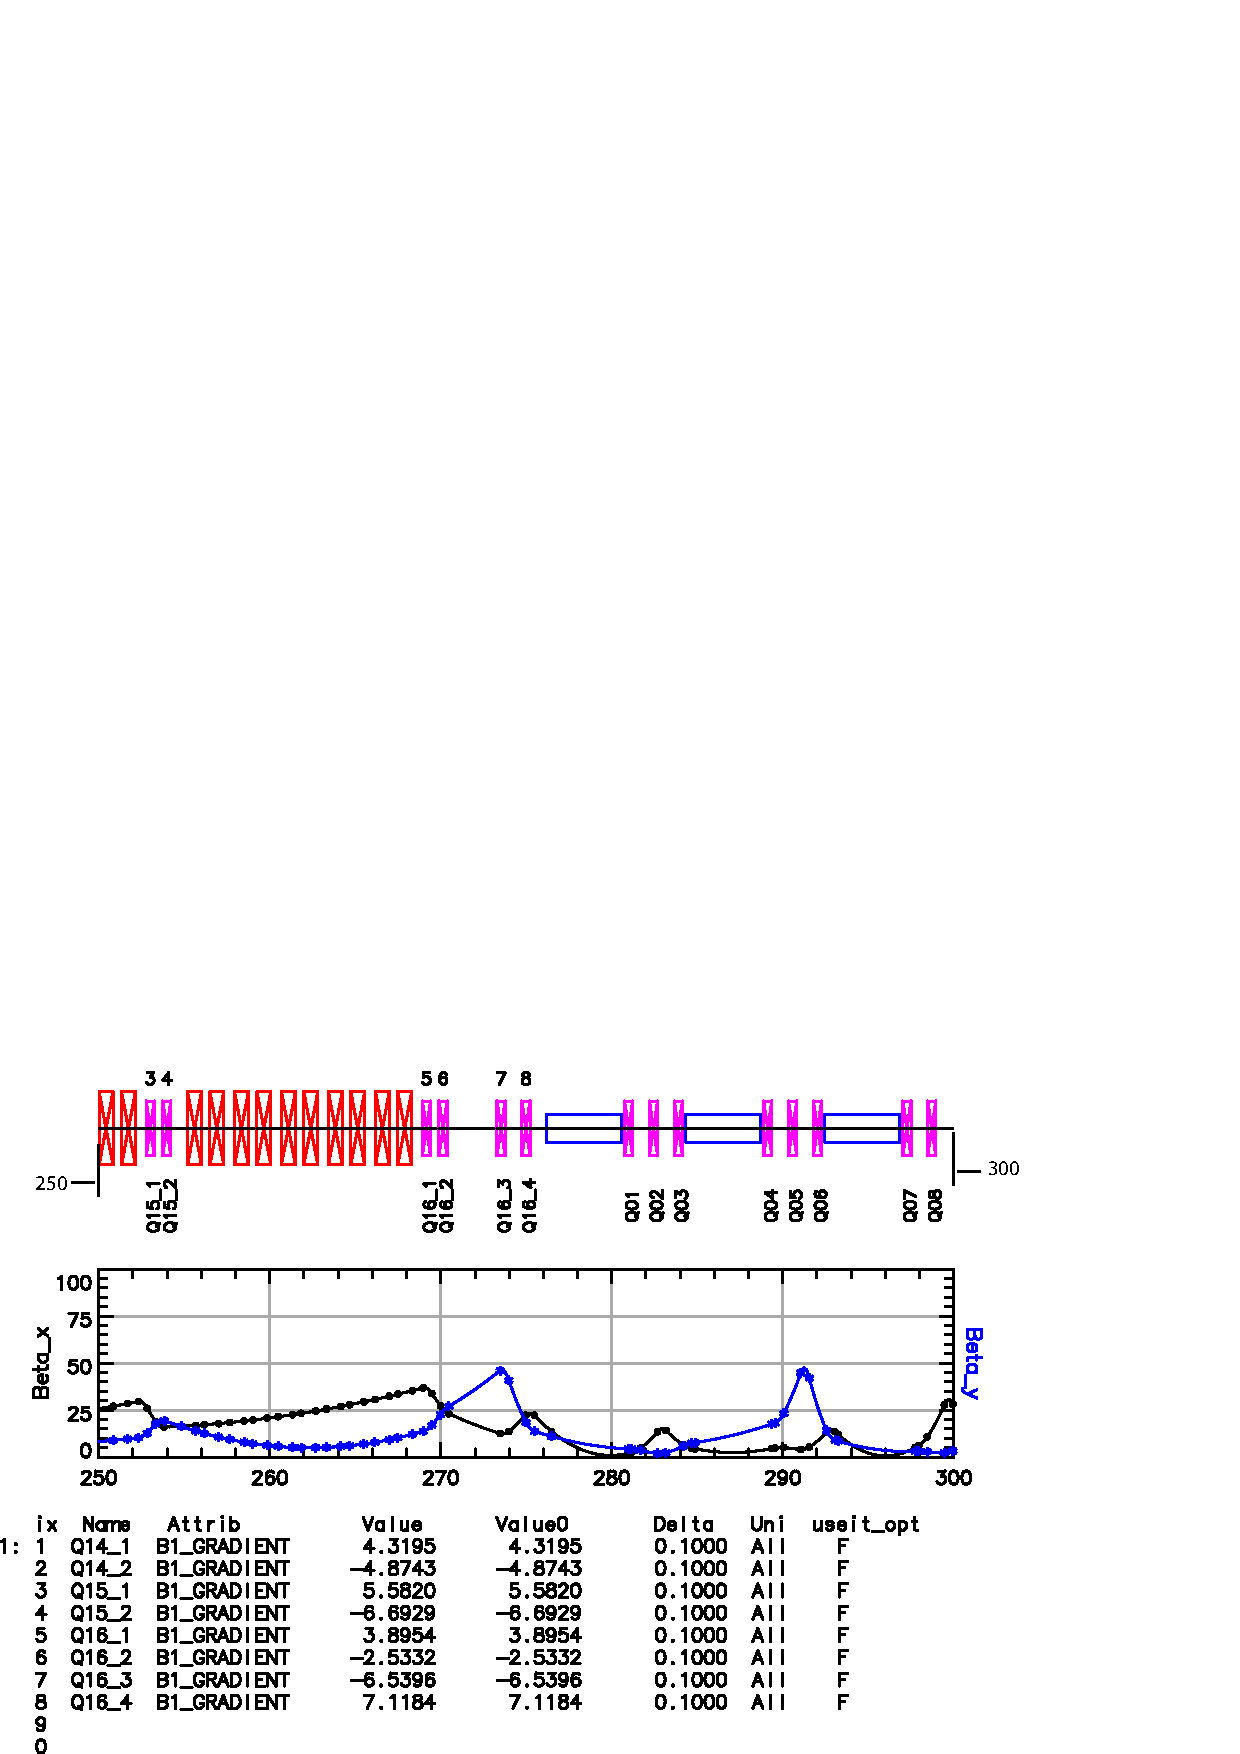
\includegraphics[width=5in]{layout-graph-table.pdf}
  \caption[Example key table with a lattice layout and data plots.]
{A lattice layout plot (top) above a data plot (middle) which in turn is above a key table plot
(bottom). Elements that have attributes that are varied as shown in the key table have the
corresponding key table number printed above the element's glyph in the lattice layout.}
  \label{f:key.table}
\end{figure}

\index{key bindings}
The main purpose of Single Mode is to associate certain keyboard keys with certain variables so that
the pressing of these keys will change their associated model value of the variable as illustrated
in Figure~\ref{f:keyboard}. This is called a \vn{key binding}. Key bindings are established in a
startup file by setting the \vn{var(i)%key_bound} and \vn{var(i)%key_delta} parameters (see
Section~\sref{s:init.var}). After startup, associated variables with keyboard keys can be done using
the \vn{set variable} command (\sref{s:set}).

The variables are divided into banks of 10. The 0\Th bank uses the first ten variables that have
their \vn{key_bound} attribute (\sref{s:init.var}) set to True.  the 1\St bank uses the next ten,
etc.  At any one time, only one bank is active. To see the status of this bank, a \vn{key_table}
plot (\sref{s:key.table})can be setup as shown in Figure~\ref{f:key.table}. The relationship between
the keys and a change in a variable is:
\begin{example}
                 Change by factor of:          
     Variable    -10  -1    1     10
   ----------    ---  ---  ---  -------
    1 + 10*ib     Q    q    1   shift-1   ("!")
    2 + 10*ib     W    w    2   shift-2   ("@")
    3 + 10*ib     E    e    3   shift-3   ("\#")
    4 + 10*ib     R    r    4   shift-4   ("\$")
    5 + 10*ib     T    t    5   shift-5   ("%")
    6 + 10*ib     Y    y    6   shift-6   ("^")
    7 + 10*ib     U    u    7   shift-7   ("\&")
    8 + 10*ib     I    i    8   shift-8   ("*")
    9 + 10*ib     O    o    9   shift-9   ("(")
   10 + 10*ib     P    p    0   shift-0   (")")
\end{example}
In the above table ib is the bank number (0 for the
0\Th bank, etc.), and the change is in multiples of the \vn{step} (\sref{s:init.var}).  value for a
variable. Note: In \vn{line mode}, the command \vn{show key_bindings} (\sref{s:show}) may be used to
show the entire set of bound keys.

Initially the 0\Th bank is active. The left arrow and right arrow are used to decrease or increase
the bank number.  Additionally the "\vn{<}" and "$>$" keys can be used to change the deltas for the
variables.

For example, looking at Figure~\ref{f:key.table}, the \vn{"1:"} in the upper left corner of the
\vn{Key Table} shows that the 1\St bank is active. \vn{key(14)} is associated with the \vn{"4"} key
and from the \vn{Key Table} it is seen that the bound attribute is the \vn{b1_gradient} of the
element named \vn{Q15_2}.  Thus, if the \vn{"4"} key is depressed in single mode, the value of the
\vn{b1_gradient} of element \vn{Q15_2} will be increased by the given Delta (0.1000 in this
case). Pressing the \vn{"r"} key (which is just below the \vn{"4"} key) will decrease the value of
the \vn{b1_gradient} by 0.1000. Using the shift key, which is shift-4 (\vn{"\$"}) will increase
\vn{b1_gradient} by 10 times the given delta (1.000 in this case) and \vn{"R"} will decrease, by a
factor of 10, the given delta.

Since element \vn{Q15_2} is also displayed in the \vn{Lattice Layout}, there is a \vn{"4"} drawn
above this element that reflects the fact that the element contains a bound attribute. Since, in
this case, the Lattice Layout only shows part of the lattice, not all key indexes are present.

%------------------------------------------------------------------------

%% keys ------------------------------------------------------------------------
\section{List of Key Strokes}\index{single mode!list of Key strokes}
\label{s:keys}

In the following list, certain commands use multiple key strokes. For example, the \vn{"/v"} command
is invoked by first pressing the slash (\vn{"/"}) key followed by the \vn{"v"} key. \vn{"a
$<$left_arrow$>$"} represents pressing the \vn{"a"} key followed by the left-arrow key.

Additionally, custom commands can be associated with any key using the \vn{set key} command
\sref{s:set}. Example:
\begin{example}
  set key h = veto var *  ! This sets the "h" key to the command "veto var *"
\end{example}

\begin{description}
\item[?]
Type a short help message.

\item[a $<$left\_arrow$>$]
Pan plots left by half the plot width.

\item[a $<$right\_arrow$>$]
Pan plots right by half the plot width.

\item[a $<$up\_arrow$>$]
Pan plots up by half the plot height.

\item[a $<$down\_arrow$>$]
Pan plots down by half the plot height.

\item[s $<$left\_arrow$>$]
Scale x-axis of plots by a factor of 2.0.

\item[s $<$right\_arrow$>$]
Scale x-axis of plots by a factor of 0.5

\item[s $<$up\_arrow$>$]
Scale y-axis of plots by a factor of 2.0.

\item[s $<$down\_arrow$>$]
Scale y-axis of plots by a factor of 0.5


\item[z $<$left\_arrow$>$]
Zoom x-axis of plots by a factor of 2.0.

\item[z $<$right\_arrow$>$]
Zoom x-axis of plots by a factor of 0.5

\item[z $<$up\_arrow$>$]
Zoom y-axis of plots by a factor of 2.0.

\item[z $<$down\_arrow$>$]
Zoom y-axis of plots by a factor of 0.5

\item[c]  
Show constraints.

\item[g]
Go run the default optimizer (\sref{s:tao.opti}). The optimizer will run until you type a '.' (a
period).  Periodically during the optimization the variable values will be written to files, one for
each universe, whose name is \vn{tao_opt_vars\#.dat}. where \vn{\#} is the universe number.

\item[v]
Show Bmad variable values in bmad lattice format. See also the \vn{/v} command. Equivalent to
\vn{show vars -bmad} in line mode.

\item[V] 
Same an \vn{v} except only variables currently enabled for optimization are shown.
This is equivalent to \vn{show vars -bmad -good} in line mode.

\item[Z] 
Go back to \vn{line mode}

\item[$<$]
Reduce the deltas (the amount that a variable is changed when you use
the keys 0 through 9) of all the variables by a factor of 2.

\item[$>$]
Increase the deltas (the amount that a variable is changed when you
use the keys 0 through 9) of all the variables by a factor of 2.

\item[$<$left\_arrow$>$]
Shift the active key bank down by 1: ib -$>$ ib - 1

\item[$<$right\_arrow$>$]
Shift the active key bank up by 1: ib -$>$ ib + 1

\item[/$<$up\_arrow$>$]
Increase all key deltas by a factor of 10.

\item[/$<$down\_arrow$>$]
Decrease all key deltas by a factor of 10.

\item[$<$CR$>$]
Do nothing but replot.

\item[-p]
Toggle plotting. Whether to plot or not to plot is initially determined by \vn{plot%enable}.

\item['$<$command$>$]
Accept a Line Mode (\sref{c:command}) command.

\item[/b]
Switch the default lattice branch (\sref{s:lattice}).

\item[/e $<$Index or Name$>$]
Prints info on a lattice element. If there are two lattices being used and only the information of
an element from one particular lattice is wanted then prepend with "n@" where n is the lattice
index.

\item[/l]
Print a list of the lattice elements with Twiss parameters.

\item[/u $<$Universe Index$>$]
Switch the default universe (\sref{s:universe}).

\item[/v]
Write variable values to the default output file in Bmad lattice format.  The default output file
name is set by \vn{global%var_out}.  See also the \vn{V} command.

\item[/x $<$min$>$ $<$max$>$]
Set the horizontal scale min and max values for all the plots. This is the same as setting
\vn{default_graph%x%min} and \vn{default_graph%x%max} in the \tao input file. If \vn{min} and
\vn{max} are not given then the scale will be chosen to include the entire lattice.

\item[/y $<$min$>$ $<$max$>$]
Set the y-axis min and max values for all the plots. This is the same as setting \vn{plot%y%min} and
\vn{plot%y%max} in the \tao input file. If \vn{min} and \vn{max} are not given then an autoscale
will be done.

\item[=v $<$digit$>$ $<$value$>$]
Set variable value. \vn{<digit>} is between 0 and 9 corresponding to a
variable of the current bank. \vn{<value>} is the value to set the
variable to.

\item[=$<$right\_arrow$>$]
Set saved ("value0") values to variable values to saved values. The saved values (the value0 column
in the display) are initially set to the initial value on startup. There are saved values for both
the manual and automatic variables. Note that reading in a TOAD input file will reset the saved
values. If you want to save the values of the variables in this case use "/w" to save to a file. Use
the "\vn{/$<$left_arrow$>$}" command to go in the reverse direction.

\item[=$<$left\_arrow$>$]
Paste saved (\vn{value0} column in the display) values back to the variable values.  The saved
values are initially set to the initial value on startup. Use the "\vn{/$<$right_arrow$>$}" command
to go in the reverse direction.

\end{description}


%----------------------------------------------------------------
\part{Programmer's Guide}

\chapter{Customizing Tao}
\index{customizing}
\label{c:custom.tao}

\tao has been designed to be readily extensible with a minimum of effort when certain rules are
followed. This chapter discusses how this is done. This is separate from using \tao's \vn{pipe}
command (\sref{s:pipe.cmd}) to control \tao.

%----------------------------------------------------------------
\section{Initial Setup}
\label{s:cust.init}

Creating a custom version of \tao involves creating custom code that is put in a directory that is
distinct from the \vn{tao} directory that contains the standard \tao code files.

\textbf{It is important to remember that the code in the \vn{tao} directory is not to be modified.
This ensures that, as time goes on, and as \tao is developed by the "Taoist" developers, changes to
the code in the \vn{tao} directories will have a minimal chance to break your custom code.} If you do
feel you need to change something in the \vn{tao} directory, please seek help first.

To setup a custom \tao version do the following:
  \begin{enumerate}
  \item
Establish a base directory in which things will be built. This directory can have any name. Here we
will call this directory \vn{ROOT}.
  \item
Make a subdirectory of \vn{ROOT} that will contain the custom code.  This directory can have any
name.  Here this directory will be called \vn{tao_custom}.
  \item
Copy the files from the directory \vn{tao/customization} to \vn{ROOT/tao_custom}. The \vn{tao}
directory is part of the \bmad package. If you do not know where to find it, ask your local Guru
where it is. Along with a \vn{README} file, there are two CMake\footnote
  {
CMake is a program used for compiling code.
  } 
script files in the \vn{customization} directory:
\begin{example}
  CMakeLists.txt
  cmake.custom_tao
\end{example}
These scripts are setup to make an executable called \vn{custom_tao}. This name can be changed by
modifying the \vn{cmake.custom_tao} file.
  \item
Copy the file \vn{tao/program/tao_program.f90} to \vn{ROOT/tao_custom}.
  \item
Copy as needed \vn{hook} files from \vn{tao/hook} to \vn{ROOT/tao_custom}. The hook files you will
need are the hook files you will want to modify to customize \tao. See below for details. See
\sref{s:cust.example} for an example.
  \item
Go to the \vn{ROOT/tao_custom} directory and use the command \vn{mk} to create the
executable 
\begin{example}
    \vn{ROOT/production/bin/custom_tao}. 
\end{example}
If a debug executable is wanted, the command \vn{mkd} will create one at: 
\begin{example}
    \vn{ROOT/debug/bin/custom_tao}
\end{example}
	\end{enumerate}
A debug executable is only needed if you are debugging the code. The debug exe will run much
slower than the production version.

%----------------------------------------------------------------
\section{It's All a Matter of Hooks}
\index{customizing!hooks}

The golden rule when extending \tao is that you are only allowed to customize routines that have the
name ``hook'' in them. These files are located in the directory \vn{tao/hook}.  To customize one of
these files, copy it from \vn{tao/hook} to \vn{ROOT} and then make modifications to the copy.

The reason for this golden rule is to ensure that, as time goes by, and revisions are made to the
\tao routines to extend \tao's usefulness and to eliminate bugs, these changes will have a minimum
impact on the specialized routines you write.  What happens if the modification you want to do
cannot be accomplished by customizing a hook routine? The answer is to contact the \tao programming
team and we will modify \tao and provide the hooks you need so that you can then do your
customization.

%----------------------------------------------------------------
\section{Implementing a Hook Routine in Tao}

Function pointers are used by \tao to call customized hook routines. \tao uses the same system as
\bmad where an abstract interface with a \vn{_def} suffix in the name is defined along with a
function pointer with a \vn{_ptr} suffix. For example, the \vn{tao_hook_command} routine has
the function pointer (defined in \vn{/tao/code/tao_interface.f90}):
\begin{example}
  procedure(tao_hook_command_def), pointer :: tao_hook_command_ptr => null()
\end{example}
To use a customized \vn{tao_hook_command} routine, the following can be put in the
\vn{tao_program.f90} that was copied to your area:
\begin{example}
  tao_hook_command_ptr => tao_hook_command
\end{example}
{\bf Important:} To not duplicate documentation, full details on setting up a hook routine is in the
section ``Custom and Hook Routines'' in the \bmad manual. Please read this.

%----------------------------------------------------------------
\section{Initializing Hook Routines}

One way to initialize a hook routine is to read in parameters from an initialization file.  If an
initialization file is used, the filename may be set using the \vn{s%global%hook_init_file}
string. This string may be set in the \vn{tao_params} namelist (\sref{s:globals}) or may be set on
the command line using the \vn{-hook_init_file} option (\sref{s:command.line}).

%----------------------------------------------------------------
\section{Hook Routines}

To get a good idea of how \tao works it is recommended to spend a little bit of time going through
the source files. This may also provide pointers on how to make customizations in the hook
routines. Of particular interest is the module \vn{tao_lattice_calc_mod.f90} where tracking and
lattice parameters are computed.

Plotting is based upon the \vn{quick_plot} subroutines which are documented in the \bmad reference
manual. If custom plotting is desired this material should be reviewed to get familiar with the
concepts of ``graph'', ``box'', and ``page''.

The following is a run through of each of the hook routines. Each routine is in a separate file
called \vn{tao/hook/<hook_routine_name>.f90}. See these files for subroutine headers and plenty of
comments throughout the dummy code to aid in the modification of these subroutines.

%-----------------------------------------------------------------
\subsection{tao_hook_branch_calc}
\index{customizing!tao_hook_branch_calc}

This hook routine is called by tao_lattice_calc when tracking, twiss calculations, etc are done.

This subroutine can be used, for example, to do custom calculations on a lattice branch.
Also see tao_hook_lattice_calc.

%-----------------------------------------------------------------
\subsection{tao_hook_command}\index{customizing!tao_hook_commad}
\label{s:hook.command}

Any custom commands are placed here. The dummy subroutine already has a bit of code that replicates
what is performed in \vn{tao_command}. Commands placed here are searched before the standard \tao
commands. This allows for the overwriting of any standard \tao command.

By default, there is one command included in here: \vn{`hook'}. This is just a simple command that
doesn't really do anything and is for the purposes of demonstrating how a custom command would be
implemented.

The only thing needed to be called at the end of a custom command is \vn{tao_cmd_end_calc}. This
will perform all of the steps listed in Section~\sref{s:lat.calc}.

See Sec.~\sref{s:cust.read.example} for an example of how to use this hook.

%-----------------------------------------------------------------
\subsection{tao_hook_data_sanity_check}
\index{customizing!tao_hook_data_sanity_check}

Hook routine to check if a custom datum is internally consistent.
This routine is called by tao_data_sanity_check. See this routine for more details.

%-----------------------------------------------------------------
\subsection{tao_hook_draw_floor_plan}
\index{customizing!tao_hook_draw_floor_plan}

Routine to customize the plotting of the floor_plan.
Also see: tao_hook_draw_graph.

%-----------------------------------------------------------------
\subsection{tao_hook_draw_graph}
\index{customizing!tao_hook_draw_graph}

This will customize the plotting of a graph. See the \tao module \vn{tao_plot_mod} for details on
what it normally done. You will also need to know how \vn{quick_plot} works (See the \bmad manual).

%-----------------------------------------------------------------
\subsection{tao_hook_evaluate_a_datum}
\index{customizing!tao_hook_evaluate_a_datum}

Any custom data types are defined and calculated here. If a non-standard data type is listed in the
initialization files, then a corresponding data type must be placed in this routine. The tutorial
uses this hook routine when calculating the emittance.

Dependent lattice parameters (such as closed orbits, beta functions, etc.) are recalculated every
time \tao believes the lattice has changed (for example, after a \vn{change} command).  This is done
in \vn{tao_lattice_calc}. \vn{tao_lattice_calc} in turn calls \vn{tao_evaluate_a_datum} for each
datum. \vn{tao_evaluate_a_datum} in turn calls \vn{tao_hook_evaluate_a_datum} to allow for custom
data evaluations. 

See the \vn{tao_evaluate_a_datum} routine as an example as how to handle datums.  The arguments for
\vn{tao_hook_evaluate_a_datum} is
\begin{example}
  tao_hook_evaluate_a_datum (found, datum, u, tao_lat, datum_value, valid_value)
\end{example}
The \vn{found} logical argument should be set to \vn{True} for datums that are handled by this hook
routine and \vn{found} should be set to \vn{False} for all other datums.

%-----------------------------------------------------------------
\subsection{tao_hook_graph_postsetup}
\index{customizing!tao_hook_graph_postsetup}


%-----------------------------------------------------------------
\subsection{tao_hook_graph_setup}
\index{customizing!tao_hook_graph_data_setup}

Use this to setup custom graph data for a plot.

%-----------------------------------------------------------------
\subsection{tao_hook_init1 and tao_hook_init2}
\label{s:hook.init}
\index{customizing!tao_hook_init}

After the \vn{design} lattice and the global and universe structures are initialized,
\vn{tao_hook_init1} is called from the \vn{tao_init} routine. Here, any further initializations can
be added. In particular, if any custom hook structures need to be initialized, here's the place to
do it.

Further down in \vn{tao_init}, \vn{tao_hook_init2} is called. Normally you will want to use
\vn{tao_hook_init1}. However, \vn{tao_hook_init2} can be used, for example, ! to set model variable
values different from design variable values since when \vn{tao_hook_init1} is called the \vn{model}
lattice has not yet been initialized.

%-----------------------------------------------------------------
\subsection{tao_hook_init_beam}
\index{customizing!tao_hook_init_beam}

%-----------------------------------------------------------------
\subsection{tao_hook_init_data}
\index{customizing!tao_hook_init_data}

%-----------------------------------------------------------------
\subsection{tao_hook_init_global}
\index{customizing!tao_hook_init_global}

%-----------------------------------------------------------------
\subsection{tao_hook_init_lattice_post_parse}
\index{customizing!tao_hook_init_lattice_post_parse}

This will do a custom lattice initialization. The standard lattice initialization just calls
\vn{bmad_parser}. If anything more complex needs to be done then do it here. This is also where any
custom overlays or other elements would be inserted after the parsing is complete. But in general,
anything placed here should, in principle, be something that can be placed in a lattice file.

\textbf{This is the only routine that should insert elements in the ring}. This is because the \tao
data structures use the element index for each element associated with the datum. If all the element
indexes shift then the data structures will break. If new elements need to be inserted then modify
this routine and recompile. You can alternatively create a custom initialization file used by this
routine that reads in any elements to be inserted.

%-----------------------------------------------------------------
\subsection{tao_hook_init_plotting}
\index{customizing!tao_hook_init_plotting}


%-----------------------------------------------------------------
\subsection{tao_hook_init_read_lattice_info}
\index{customizing!tao_hook_init_read_lattice_info}

%-----------------------------------------------------------------
\subsection{tao_hook_init_var}
\index{customizing!tao_hook_init_read_lattice_info}

%-----------------------------------------------------------------
\subsection{tao_hook_lattice_calc}
\index{customizing!tao_hook_lattice_calc}

The standard lattice calculation can be performed for single particle, particle beam tracking and
will recalculate the orbit, transfer matrices, twiss parameters and load the data arrays. If
something else needs to be performed whenever the lattice is recalculated then it is placed here. A
custom lattice calculation can be performed on any lattice separately, this allows for the
possibility of, for example, tracking a single particle for one lattice and beams in another.

%-----------------------------------------------------------------
\subsection{tao_hook_merit_data}
\index{customizing!tao_hook_merit_data}

A custom data merit type can be defined here. Table~\ref{t:delta.v} lists the standard merit
types. If a custom merit type is used then \vn{load_it} in \vn{tao_hook_load_data_array} may also
need to be modified to handle this merit type, additionally, all standard data types may need to be
overridden in \vn{tao_hook_load_data_array} in order for the custom \vn{load_it} to be used.  See
\vn{tao_merit.f90} for how the standard merit types are calculated.

%-----------------------------------------------------------------
\subsection{tao_hook_merit_var}
\index{customizing!tao_hook_merit_var}

This hook will allow for a custom variable merit type. However, since there is no corresponding data
transfer, no \vn{load_it} routine needs to be modified.  See \vn{tao_merit.f90} for how the standard
merit types are calculated.

%-----------------------------------------------------------------
\subsection{tao_hook_optimizer}
\index{customizing!tao_hook_optimizer}

If a non standard optimizer is needed, then it can be implemented here. See the
\vn{tao_*_optimizer.f90} files for how the standard optimizers are implemented.

%-----------------------------------------------------------------
\subsection{tao_hook_parse_command_args}
\index{customizing!tao_hook_parse_command_args}

The \vn{tao_hook_parse_command_args} routine can be used to set the names of initialization
files. The file names are stored in the \vn{s%com} structure. For example, in the hook file, the
following changes the default plot initialization file:
\begin{example}
  s%com%hook_plot_file = '/nfs/acc/user/dcs16/my_plot_init.tao'
\end{example}
Note that if an initialization file name is given on the command line or in the root \tao
initialization file, that name will supersede the hook name.

%-----------------------------------------------------------------
\subsection{tao_hook_plot_setup}
\index{customizing!tao_hook_plot_setup}

Use this routine to override the \vn{tao_plot_data_setup} routine which essentially transfers the
information from the \vn{s%u(:)%data} arrays to the
\vn{s%plot_page%region(:)%plot%graph(:)%curve(:)} arrays. This may be useful if you want to make a
plot that isn't simply the information in a data or variable array.




%-----------------------------------------------------------------
\subsection{tao_hook_post_process_data}
\index{customizing!tao_hook_post_process_data}

Here can be placed anything that needs to be done after the data arrays are loaded. This routine is
called immediately after the data arrays are called and before the optimizer or plotting is done, so
any final modifications to the lattice or data can be performed here.

%-----------------------------------------------------------------
\subsection{tao_hook_show_cmd}
\index{customizing!tao_hook_show_cmd}

%-----------------------------------------------------------------
%\chapter{Plotting}
%\label{s:prog.plotting} 

%\fbox{this chapter is yet to be completed!} 

%----------------------------------------------------------------
\section{Adding a New Data Type Example}
\label{s:cust.example}

As an example of a customization, let's include a new data type called \vn{particle_emittance}. This
will be the non-normalized x and y emittance as found from the Courant-Snyder invariant. This data
type will behave just like any other data type (i.e.  \vn{orbit}, \vn{phase} etc...).

This example will only require the modification of one file:
\vn{tao_hook_evaluate_a_datum.f90}. This file should be copied from the \vn{tao/hook} directory and
put in your \vn{ROOT/code} directory (\sref{s:cust.init}).

The formula for single particle emittance is
\begin{equation}
  \epsilon = \gamma x^{2} + 2 \alpha x x' + \beta x'^{2}
  \label{e:emittance}
\end{equation}
Place the following code in \vn{tao_hook_evaluate_a_datum.f90} in the \cmd{case select}
construct. Also add the necessary type declarations. See the routine \vn{tao_evaluate_a_datum} as an
example.
\begin{example}
  type (coord_struct), pointer :: orbit(:)
  type (ele_struct), pointer :: ele
  type (lat_struct), pointer :: lat
  integer ix_ele
  ...
  lat => tao_lat%lat
  orbit => tao_lat%tao_branch(0)%orbit
  ele => tao_pointer_to_datum_ele (lat, datum%ele_name, datum%ix_ele, datum, &
                                                          valid_value, why_invalid)
  ...
  select case (datum%data_type)
  case ('particle_emittance.x') 
    datum_value =  (ele%a%gamma * orbit(ix_ele)%vec(1)**2 + &
		     2 * ele%a%alpha * orbit(ix_ele)%vec(1) * orbit(ix_ele)%vec(2) + &
		     ele%a%beta * orbit(ix_ele)%vec(2)**2)
    
  case ('particle_emittance.y')
    datum_value = (ele%b%gamma * orbit(ix_ele)%vec(3)**2 + &
		     2 * ele%b%alpha * orbit(ix_ele)%vec(3) * orbit(ix_ele)%vec(4) + &
		     ele%b%beta * orbit(ix_ele)%vec(4)**2)
  end select
\end{example}
This defines what is to be calculated for each \vn{particle_emittance} datum.  There are two
transverse coordinates, so two definitions need to be made, one for each dimension.

Now you just need to declare the data types in the \cmd{tao.init} and \cmd{tao_plot.init} files. For
the sake of this example, modify the example files found in the \vn{bmad-doc/tao_examples} directory
\begin{example}
	mkdir ROOT/my_example
  cp tao/example/*.init ROOT/my_example
  cp tao/example/*.lat ROOT/my_example
\end{example}

In \cmd{ROOT/my_example/tao.init} add the following lines to the data declarations section
\begin{example}
  &tao_d2_data
    d2_data%name = "particle_emittance" 
    universe = 0 
    n_d1_data = 2
  /

  &tao_d1_data
    ix_d1_data = 1
    d1_data%name = "x"  
    default_weight = 1
    use_same_lat_eles_as = 'orbit.x"
  /

  &tao_d1_data
    ix_d1_data = 2
    d1_data%name = "y"  
    default_weight = 1
    use_same_lat_eles_as = 'orbit.x"
  /
\end{example}

In \cmd{ROOT/my_example/tao_plot.init} add the following lines to the end
of the file
\begin{example}
  &tao_template_plot
    plot%name = 'particle_emittance'
    plot%x_axis_type = 'index'
    plot%n_graph = 2
  /
  
  &tao_template_graph
    graph%name = 'x'
    graph_index = 1
    graph%box = 1, 2, 1, 2
    graph%title = 'Horizontal Emittance (microns)'
    graph%margin =  0.15, 0.06, 0.12, 0.12, '%BOX'
    graph%y%label = 'x'
    graph%y%max =  15
    graph%y%min =  0.0
    graph%y%major_div = 4
    curve(1)%data_source = 'data'
    curve(1)%data_type   = 'particle_emittance.x'
    curve(1)%y_axis_scale_factor = 1e6 !convert from meters to microns
  /

  &tao_template_graph
    graph%name = 'y'
    graph_index = 2
    graph%box = 1, 1, 1, 2
    graph%title = 'Vertical Emittance (microns)'
    graph%margin =  0.15, 0.06, 0.12, 0.12, '%BOX'
    graph%y%label = 'Y'
    graph%y%max =  15
    graph%y%min =  0.0
    graph%y%major_div = 4
    curve(1)%data_source = 'data'
    curve(1)%data_type = 'particle_emittance.y'
    curve(1)%units_factor = 1e6 !convert from meters to microns
  /
\end{example}
These namelists are described in detail in Chapter~\ref{c:init}.

We are now ready to compile and then run the program. The \tao library should have already been
created so all you need to do is
\begin{example}
	cd ROOT/code
	mk
  cd ROOT/my_example
  ../production/bin/custom_tao
\end{example}

After your custom \tao initializes type
\begin{example}
  place bottom particle_emittance
  scale
\end{example}
Your plot should look like Figure~\ref{f:plot.emittance}.

The emittance (as calculated) is not constant. This is due to dispersion and coupling throughout the
ring. \bmad provides a routine to find the particle emittance from the twiss parameters that
includes dispersion and coupling called \vn{orbit_amplitude_calc}.

\begin{figure}
  \centering
  \includegraphics[width=5in]{plot-emittance.pdf}
  \caption{Custom data type: non-normalized emittance}
  \label{f:plot.emittance}
\end{figure}

%----------------------------------------------------------------
\section{Reading in Measured Data Example}
\label{s:cust.read.example}

This section shows how to construct a customized version of \tao, called \vn{ping_tao}, to read in
measured data for analysis. This example uses data from the Fermilab proton recirculation. The data
is obtained by measuring the orbit turn-by-turn of a beam that has been initially pinged to give it
a finite oscillation amplitude.

The files for constructing \vn{ping_tao} can be found
in the directory
\begin{example}
  bmad-doc/tao_examples/custom_tao_with_measured_data
\end{example}
The files in this directory are as follows:
\begin{description}
  \item[CMakeLists.txt, cmake.ping_tao] \Newline
Script files for creating \vn{ping_tao}. See Sec.~\sref{s:cust.init}.
  \item[README] \Newline
The \vn{README} file gives some instructions on how to create \vn{ping_tao}
  \item[RRNOVAMU2E11172016.bmad] \Newline
Lattice file for the proton recirculation ring.
  \item[data] \Newline
Directory where some ping data is stored
  \item[tao.init] \Newline
\tao initialization file defining the appropriate data and variable structures (\sref{s:init.begin})
  \item[tao.startup] \Newline
File with some command that are executed when \tao is started. These commands will read in
and plot some data.
  \item[tao_hook_command.f90] \Newline
Custom code for reading in ping data. The template used to construct this file is at
\vn{tao/hook/tao_hook_command.f90} (\sref{s:hook.command}).
  \item[tao_plot.init] \Newline
File for defining plot parameters (\sref{s:init.plot}).
  \item[tao_program.f90] \Newline
copy of the \vn{tao/program/tao_program.f90} file (\sref{s:cust.init}).
\end{description}

After creating the \vn{ping_tao} program (see the \vn{README} file), the program can be run by going
to the custom_tao_with_measured_data directory and using the command:
\begin{example}
	../production/bin/ping_tao
\end{example}

The customized \vn{tao_hook_command} routine implements a custom command called
\vn{pingread}.  This command will read in ping data. Ping data is the amplitude and phase
of the beam oscillations at a BPM for either the \vn{a-mode} or \vn{b-mode} oscillations.
See the write up on ping data types in Sec.~\sref{s:data.types} under \vn{ping_a.amp_x},
and \vn{ping_b.amp_x} for more details.

The data files in the \vn{data} directory contain data for either the \vn{a-mode} or \vn{b-mode}
ping at either the horizontal or vertical BPMs.

The syntax of the \vn{pingread} command is:
\begin{example}
  pingread <mode> <filename> <data_or_ref>
\end{example}
The first argument, \vn{<mode>}, should be either ``\vn{a_mode}'' ``\vn{b_mode}'' indicating wether
the data is for the \vn{a-mode} \vn{b-mode} analysis (a better setup would encode this information
in the data file itself). The second argument, \vn{filename} is the name of the data file, and the
third argument, \vn{data_or_ref} should be ``\vn{data}'' or ``\vn{reference}'' indicating that the
data is to be read into the \vn{meas_value} or \vn{ref_value} of the appropriate
\vn{tao_data_struct}.

%----------------------------------------------------------------
\subsection{Analysis of the tao_hook_command.f90 File}
\label{s:hook.cmd.anal}

The first part of the \vn{tao_hook_command} routine parses the command line to see if the
\vn{pingread} command is present. The relevant code, somewhat condensed, is:
\begin{example}
  subroutine tao_hook_command (command_line, found)

  !!!! put your list of hook commands in here. 

  character(16) :: cmd_names(1) = [character(16):: 'pingread']  

  ! "found" will be set to TRUE if the command is found.

  found = .false.

  ! strip the command line of comments

  call string_trim (command_line, cmd_line, ix_line)
  ix = index(cmd_line, '!')
  if (ix /= 0) cmd_line = cmd_line(:ix-1)        ! strip off comments

  ! blank line => nothing to do

  if (cmd_line(1:1) == '') return

  ! match first word to a command name
  ! If not found then found = .false.

  call match_word (cmd_line(:ix_line), cmd_names, ix_cmd, .true., .true., cmd_name)
  if (ix_cmd < 0) then
    call out_io (s_error$, r_name, 'AMBIGUOUS HOOK COMMAND')
    found = .true.
    return
  endif

  found = .true.
  call string_trim (cmd_line(ix_line+1:), cmd_line, ix_line)
\end{example}

Note: To quickly find information on routines and structures, use the \vn{getf} and \vn{listf}
scripts as explained in the \bmad manual. For example, typing ``\vn{getf string_trim}'' on the
system command line will give information on the string_trim subroutine.

The above code tests to see if the command is \vn{pingread} and, if not, returns without doing
anything.

If the \vn{pingread} command is found, the rest of the command line is parsed to get the
\vn{<mode>}, \vn{<filename>}, and \vn{<data_or_ref>} arguments.

In the \vn{tao.init} file, a \vn{tune} d2 datum is setup to have two \vn{d1} datum arrays One for
the \vn{a}-mode tune and one for the \vn{b}-mode tune:
\begin{example}
  \&tao_d2_data
    d2_data%name = "tune"
    universe = '*'  ! apply to all universes
    n_d1_data = 2
  /

  \&tao_d1_data
    ix_d1_data = 1
    d1_data%name = "a"
    default_weight = 1e6
    ix_min_data = 1
    ix_max_data = 1
  /

  \&tao_d1_data
    ix_d1_data = 2
    d1_data%name = "b"
    default_weight = 1e6
    ix_min_data = 1
    ix_max_data = 1
  /
\end{example}
And each \vn{d1} array has only one datum since the \vn{a}-mode and \vn{b}-mode tunes have only one
value associated with them (as opposed to, say an orbit which will have multiple values from
different BPMs).

In a data file there is a header section which, among other things, records the tune.
In a line beginning with the word ``\vn{Tune}''. Example:
\begin{example}
                   Horz         Vert         Sync.                           
   Tune           ( .452444)   ( .404434)   ( 0      ) 2p                    
\end{example}

In the \vn{tao_hook_command} file, after the arguments are parsed, the header part of the
data file is read to extract the tune datums:
\begin{example}
  type (tao_d2_data_array_struct), allocatable :: d2(:)
  ...
  if (line(1:4) == 'Tune') then
    call tao_find_data (err, 'tune', d2_array = d2)
    if (size(d2) /= 1) then
      call out_io (s_fatal$, r_name, 'NO TUNE D2 DATA STRUCTURE DEFINED!')
      return
    endif
\end{example}
The call to \vn{tao_find_data} looks for a \vn{d2} data structure named \vn{tune}. This structure is
setup in the \vn{tao.init} file. Alternatively, the \vn{ping_tao} program could be configured to
automatically setup the appropriate data and/or variable structures via the \vn{tao_hook_init1}
routine (\sref{s:hook.init}).

The returned value from the call to \vn{tao_find_data} is an array called \vn{d2} of type
\vn{tao_d2_data_array_struct}. \vn{d2} holds an array of pointers to all \vn{d2_data_struct}
structures it can find. In general, there could be multiple such structures if multiple universes
are being used or if the match string, in this case \vn{'tune'}, contained wild card characters. In
this case, the expectation is that there will only one universe used and thus there should be one
and only one structure that matches the name \vn{tune}. This structure will be pointed to by
\vn{d2(1)%d2}. The appropriate datums, will be:
\begin{example}
  d2(1)%d2%d1(1)%d(1)   ! a-mode tune
  d2(1)%d2%d1(1)%d(2)   ! b-mode tune
\end{example}
The values read from the data file are put in these datums via the code:
\begin{example}
  if (data_or_ref == 'data') then
    d2(1)%d2%d1(1)%d(1)%meas_value = twopi * (data_tune_a + nint(design_tune_a))
    d2(1)%d2%d1(1)%d(1)%good_meas = .true.
    d2(1)%d2%d1(2)%d(1)%meas_value = twopi * (data_tune_b + nint(design_tune_b))
    d2(1)%d2%d1(2)%d(1)%good_meas = .true.
  else
    d2(1)%d2%d1(1)%d(1)%ref_value = twopi * (data_tune_a + nint(design_tune_a))
    d2(1)%d2%d1(1)%d(1)%good_ref = .true.
    d2(1)%d2%d1(2)%d(1)%ref_value = twopi * (data_tune_b + nint(design_tune_b))
    d2(1)%d2%d1(2)%d(1)%good_ref = .true.
  endif      
\end{example}

The next step is to setup pointers to the appropriate data arrays to receive the ping data.
In the data file the ping data looks like:
\begin{example}
  BPM           Phase    Ampl.   RMSdev     Beta  bml_psi *Calib Old_Cal     
  R:HP222    -0.27314  0.46085    0.078    1.863  0.35183                         
  R:HP224    -0.05939  0.28277    0.143    0.701 -0.43442                         
  R:HP226     0.23140  0.31712    0.075    0.882 -0.14363                         
  ... etc ...
\end{example}
The ``\vn{H}'' in \vn{R:HP222}, etc. indicates that the data is from BPMs that only measure the
horizontal displacement of the beam. Alternatively, a ``\vn{V}'' would indicate data from vertical
measurement BPMs.

In the \vn{tao_hook_command} file the data pointers are setup by the code:
\begin{example}
  type (tao_d1_data_array_struct), allocatable, target :: d1_amp_arr(:), d1_phase_arr(:)
  ...
  if (line(3:3) == 'H') then
    if (mode == 'a_mode') then
      call tao_find_data (err, 'ping_a.amp_x', d1_array = d1_amp_arr)
      call tao_find_data (err, 'ping_a.phase_x', d1_array = d1_phase_arr)
    else 
      call tao_find_data (err, 'ping_b.amp_x', d1_array = d1_amp_arr)
      call tao_find_data (err, 'ping_b.phase_x', d1_array = d1_phase_arr)
    endif
  elseif (line(3:3) == 'V') then
    if (mode == 'a_mode') then
      call tao_find_data (err, 'ping_a.amp_y', d1_array = d1_amp_arr)
      call tao_find_data (err, 'ping_a.phase_y', d1_array = d1_phase_arr)
    else 
      call tao_find_data (err, 'ping_b.amp_y', d1_array = d1_amp_arr)
      call tao_find_data (err, 'ping_b.phase_y', d1_array = d1_phase_arr)
    endif
\end{example}
\vn{line(3:3)} is either \vn{H} or \vn{V} indicating horizontal or vertical orbit measuring BPMs. In
this case, the call to the \vn{tao_find_data} routine returns \vn{d1} data arrays to the amplitude
data (\vn{d1_amp_arr}) and phase data (\vn{d1_phase_arr}).  Just like the tune data, since it is
assumed only one universe is being used, there should be one and only \vn{d1} structure for the
phase and only one \vn{d1} structure for the amplitude:
\begin{example}
  d1_amp_arr(1)%d1      ! d1 struucture for the amplitude data
  d1_phase_arr(1)%d1    ! d1 struucture for the phase data
\end{example}
To save on typing, and make the code clearer, pointers are used to point to these structures:
\begin{example}
  type (tao_d1_data_struct), pointer :: d1_phase, d1_amp
  ...
  d1_amp => d1_amp_arr(1)%d1
  d1_phase => d1_phase_arr(1)%d1
\end{example}
The array of datums for the amplitude and phase data will be \vn{d1_amp%d(:)} and
\vn{d1_phase%d(:)} respectively.

After the \vn{d1_amp} and \vn{d1_phase} pointers have been set, there is a loop over all the lines
in the file to extract the ping data. One problem faced is that the order of the data in the file is
not the same as the order of the data in \vn{d1} structures.  [The data in the file is sorded in
increasing numberical order in the BPM name while the order in the \vn{d1} structures is sorted by
increasing logitudinal s-position.]  To get around this problem, the BPM name in the file is used to
locate the appropriate datum (the associated BPM element name is stored in the \vn{%ele_name}
component of the datums):
\begin{example}
  character(140) :: cmd_word(12), ele_name
  ... 
  call tao_cmd_split (line, 4, cmd_word, .false., err)
  read (cmd_word(2), *) r1
  read (cmd_word(3), *) r2
  ele_name = cmd_word(1)
  datum_amp => tao_pointer_to_datum(d1_amp, ele_name(3:))
  datum_phase => tao_pointer_to_datum(d1_phase, ele_name(3:))
\end{example}
The \vn{line} string holds a line from the data file, the call to \vn{tao_cmd_split} splits the line
into word chunks and puts them into the array \vn{cmd_word(:)}.  \vn{cmd_word(1)} holds the first
word which is the BPM name with ``\vn{R:}'' prepended to the name. The calls to
\vn{tao_pointer_to_datum} return pointers, \vn{datum_amp} and \vn{datum_phase}, to the approbriate
datums given the BPM name.

After the appropriate datums have been identified, the ping data values read from the data
file, \vn{r1} and \vn{r2}, are used to set the appropriate components:
\begin{example}
  if (data_or_ref == 'data') then
    datum_phase%good_meas = .true.
    datum_amp%meas_value = r2
    datum_amp%good_meas = .true.
  else
    datum_phase%good_ref = .true.
    datum_amp%ref_value = r2
    datum_amp%good_ref = .true.
  endif
\end{example}

One problem is that individual data phase data points can be off by factors of $2\pi$. To correct
this, the measured phase values are shifted by factors of $2\pi$ so that they are within $\pm\pi$ of
the design values. There is an added ``branch cut'' problem here in that, even without the factors
of $2\pi$ problem, the measured phases will be off from the design values by some arbitrary amount
(determined by how the zero phase is defined in the program that created the data file). If this
difference between the zero phase of the data and the zero phase of design lattice (in the design
lattice, the phase is taken to be zero at the beginning of the lattice) is close enough to $\pi$,
the shifting of the phases by factors of $2\pi$ will not be correct. For this reason, a best guess
as to what the offset is is used in the calculation to avoid the branch cut problem:
\begin{example}
  rms_best = 1e30

  do i = 1, 20
    offset = i / 20.0
    data = data + nint(design + offset - data)
    rms = sum((data - design - offset)**2, mask = ok)
    if (rms < rms_best) then
      offset_best = offset
      rms_best = rms
    endif
  enddo

  data = data + nint(design + offset_best - data)
\end{example}

%-----------------------------------------------------------------
%\chapter{Introduction}
%\label{c:prog_intro} 

\tao has been designed to be ready extensible with a minimum of
effort. The tutorial providesa simple example of a custom data type. Here each
the hook routines are explained and pointers are given for writing code. 

\chapter{Creating a Custom Version of \tao}
\label{c:prog_intro} 

The process is summarized as follows: For the purposes of this
discussion assume that the directory that you are developing \tao in
is called \vn{ROOT}. 
\begin{enumerate}
\item 
The first step is to checkout from CVS (or download a
copy) of \tao. You will now have \tao in
\vn{ROOT/tao}. The library source code will be sitting in \vn{ROOT/tao/code}
and the vanilla \tao program is \vn{ROOT/tao/program/tao_cl.f90}
\item 
From the \vn{ROOT}/tao area build the \tao library using the
\vn{gmake} command. This will create a \tao library that includes dummy hook
routines and structures. When creating custom hooks these are overiden.
\item
To extend \tao you will want to make a new
directory, say, called \vn{ROOT/my_tao}. In this directory you write
the necessary routines to extend \tao. You will also need a standard \vn{Makefile}
 for building programs.
\item
You can compile and link your routines with the \tao routines using
\vn{gmake} in \vn{ROOT/my_tao}.
\end{enumerate}

The tutorial in Part I of this manual gave an example of how to carry out the
above steps. This is repeated below but in greater detail.

\section{Creating the \tao Library and a Custom \tao Directory}
After obtaining the \tao distribution the \tao library is created by typing 
\cmd{gmake} in the \cmd{ROOT/tao} directory. This will create two libraries
called \cmd{libtao.a} and \cmd{libtao_g.a} where the second is a debug version
in the directory \cmd{ROOT/lib}. If you then type \cmd{gmake -f M.tao} then
"vanilla" \tao will be compiled called \cmd{tao} and \cmd{tao_g} and placed in
\cmd{ROOT/bin}


\section{Modifying the Hook Routines and Structures}

The golden rule when writing routines to extend \tao is that you are
only allowed to replace routines or redefine structures that have the
name ``hook'' in them. The reason for this is to ensure that, as time
goes by, and revisions are made to the \tao routines to extend the
usefulness of \tao and to eliminate bugs, that these changes will
have a minimum impact on the specialized routines that will be written
by various people to extend \tao.  What happens if you need to replace
or modify a non--hook routine or structure?  The answer is to contact
the \tao programming team and we will modify \tao and create the hooks 
you need.

Before one can begin writing code one must understand the structures
that \tao uses. The structures are defined in a file
\vn{tao/code/tao_struct.f90}.  \tao is based upon the \bmad software
package for simulations of relativistic charged particles and the
\tao structures have components that are defined in \bmad. For
information on these structures see the \bmad Reference Manual. Note
that the hook--structures are defined in a file \vn{tao_hook_mod.f90}.

%-----------------------------------------------------------------
\chapter{Plotting}
\label{s:prog_plotting} 

Plotting is based upon the \vn{quick_plot} subroutines which are
documented in the \bmad reference manual and you should review this
material if you are not familiar with concepts of ``graph'', ``box'',
and ``page''. 

\fbox{this chapter is yet to be completed!} 




%----------------------------------------------------------------
\begin{thebibliography}{99}

\bibitem{b:coupling}
D. Sagan and D. Rubin ``Linear Analysis of Coupled Lattices,''
Phys.\ Rev.\ ST Accel.\ Beams {\bf 2}, 074001 (1999).

\bibitem{b:maduser}
H. Grote, F. C. Iselin, {\it The MAD Program User's Reference Manual},
Version 8.19, CERN/SL/90-13 (AP) (REV. 5) (1996). Can be obtained at:
$<$http://mad.home.cern.ch/mad$>$ (under MAD version 8).

\bibitem{b:madphysics}
F. C. Iselin, {\it The MAD program Physical Methods Manual}, 
unpublished, (1994).  Can be obtained at: $<$http://mad.home.cern.ch/mad$>$
(under MAD version 8).

\bibitem{b:scr}
D. Sagan, J. Crittenden, and D. Rubin.
``A Symplectic Model for Wigglers," Part.\ Acc.\ Conf. (2003).

\bibitem{b:healy}
L. M. Healy, {\it Lie Algebraic Methods for Treating Lattice Parameter
Errors in Particle Accelerators}. Doctoral thesis, University of
Maryland, unpublished, (1986).

\bibitem{b:rosenzweig}
J. Rosenzweig and L. Serafini, ``Transverse Particle Motion in
Radio--Frequency Linear Accelerators,'' Phys Rev E, Vol. 49, p. 1599,
(1994).

\bibitem{b:nr}
W. Press, B. Flannery, S. Teukolsky, and W. Wetterling, {\em Numerical
Recipes in Fortran, the Art of Scientific Computing}, Second Edition,
Cambridge University Press, New York, (1992).

\bibitem{b:nr.f90}
W. Press, B. Flannery, S. Teukolsky, and W. Wetterling, {\em Numerical
Recipes in Fortran90, the Art of Parallel Scientific Computing}, 
Cambridge University Press, New York, (1996).


\bibitem{b:boris}
P. H. Stoltz and J. R. Cary, ``Efficiency of a Boris--like Integration
Scheme with Spatial Stepping,'' Phys.\ Rev.\ Special Topics ---
Accel. \& Beams {\bf 5}, 094001 (2002).

\bibitem{wiedemann}
H. Wiedemann, {\em Particle Accelerator Physics}, Springer, New York, (1999). 

\bibitem{b:forest}
E. Forest, {\em Beam Dynamics: A New Attitude and Framework},
Harwood Academic Publishers, Amsterdam (1998).

\end{thebibliography}


\printindex

\end{document}
